%%%%%%%% ICML 2023 EXAMPLE LATEX SUBMISSION FILE %%%%%%%%%%%%%%%%%

\documentclass{article}

% Recommended, but optional, packages for figures and better typesetting:
\usepackage{microtype}
\usepackage{graphicx}
\usepackage{subfigure}
\usepackage{booktabs} % for professional tables

% hyperref makes hyperlinks in the resulting PDF.
% If your build breaks (sometimes temporarily if a hyperlink spans a page)
% please comment out the following usepackage line and replace
% \usepackage{icml2023} with \usepackage[nohyperref]{icml2023} above.
\usepackage{hyperref}

% Attempt to make hyperref and algorithmic work together better:
% \newcommand{\theHalgorithm}{\arabic{algorithm}}

% Use the following line for the initial blind version submitted for review:
% \usepackage{icml2023}

% If accepted, instead use the following line for the camera-ready submission:
\usepackage[accepted]{icml2023}

% For theorems and such
\usepackage{amsmath}
\usepackage{amssymb}
\usepackage{mathtools}
\usepackage{amsthm}

% if you use cleveref..
% \usepackage[capitalize,noabbrev]{cleveref}

%%%%%%%%%%%%%%%%%%%%%%%%%%%%%%%%
% THEOREMS
%%%%%%%%%%%%%%%%%%%%%%%%%%%%%%%%
\theoremstyle{plain}
\newtheorem{theorem}{Theorem}[section]
\newtheorem{proposition}[theorem]{Proposition}
\newtheorem{lemma}[theorem]{Lemma}
\newtheorem{corollary}[theorem]{Corollary}
\theoremstyle{definition}
\newtheorem{definition}[theorem]{Definition}
\newtheorem{assumption}[theorem]{Assumption}
\theoremstyle{remark}
\newtheorem{remark}[theorem]{Remark}

% Todonotes is useful during development; simply uncomment the next line
%    and comment out the line below the next line to turn off comments
%\usepackage[disable,textsize=tiny]{todonotes}
\usepackage[textsize=tiny]{todonotes}

\usepackage{icml2023}

% Optional math commands from https://github.com/goodfeli/dlbook_notation.
\input{math_commands.tex}

% \usepackage[hidelinks]{hyperref}
% \usepackage{url}
% \usepackage{graphicx}
\usepackage{enumitem}
\usepackage{booktabs}
\usepackage{multirow}
\usepackage{tablefootnote}


% For pseudo code
\usepackage{algorithm}
\usepackage{algorithmic}

% % For showing false positives detect
% \usepackage{listings}
% \lstset{basicstyle=\ttfamily}
%\usepackage[most]{tcolorbox}
\usepackage{tcolorbox}
\usepackage{mdframed}
\usepackage{xcolor}
\usepackage{multicol}
\usepackage{caption}
%\tcbuselibrary{minted,skins}
% \usepackage[finalizecache]{minted}
% \usepackage{minted}
\usepackage[frozencache=true,cachedir=_minted-output]{minted} 
% \usepackage[frozencache]{minted}



\usepackage{tabularx}
\usepackage{booktabs}

\usepackage{cleveref}
\tcbuselibrary{xparse,skins,breakable}

\tcbset{%
    basestyle/.style={enhanced,breakable,
        fonttitle=\scshape,
        coltitle=white},
    defstyle/.style={basestyle},
    theostyle/.style={basestyle},
}
% \DeclareTColorBox[auto counter,number within=section,crefname={example}{examples}]{example}{ o O{} t\label g }{%
%     defstyle,IfValueTF={#1}{title={Example~\thetcbcounter\ (#1)}}{title=Example~\thetcbcounter}, IfBooleanTF={#3}{label=#4}{},#2}
\DeclareTColorBox[auto counter,crefname={example}{examples}]{example}{ o O{} t\label g }{%
    defstyle,IfValueTF={#1}{title={Example~\thetcbcounter\ (#1)}}{title=Example~\thetcbcounter}, IfBooleanTF={#3}{label=#4}{},#2}

\newif\ifcomments
% comment below to remove comments, uncomment to add comments
%\commentsfalse 
\commentstrue
\ifcomments
    \newcommand{\ion}[1]{{\color{blue}{\bf\sf ion: #1]}}}

\else
    \newcommand{\ion}[1]{}
\fi

% The \icmltitle you define below is probably too long as a header.
% Therefore, a short form for the running title is supplied here:
% \icmltitlerunning{Submission and Formatting Instructions for ICML 2023}

\begin{document}

\twocolumn[
\icmltitle{Rethinking Benchmark and Contamination for Language Models with Rephrased Samples}

% It is OKAY to include author information, even for blind
% submissions: the style file will automatically remove it for you
% unless you've provided the [accepted] option to the icml2023
% package.

% List of affiliations: The first argument should be a (short)
% identifier you will use later to specify author affiliations
% Academic affiliations should list Department, University, City, Region, Country
% Industry affiliations should list Company, City, Region, Country

% You can specify symbols, otherwise they are numbered in order.
% Ideally, you should not use this facility. Affiliations will be numbered
% in order of appearance and this is the preferred way.
\icmlsetsymbol{equal}{*}

% \begin{icmlauthorlist}
% \icmlauthor{Firstname1 Lastname1}{equal,yyy}
% \icmlauthor{Firstname2 Lastname2}{equal,yyy,comp}
% \icmlauthor{Firstname3 Lastname3}{comp}
% \icmlauthor{Firstname4 Lastname4}{sch}
% \icmlauthor{Firstname5 Lastname5}{yyy}
% \icmlauthor{Firstname6 Lastname6}{sch,yyy,comp}
% \icmlauthor{Firstname7 Lastname7}{comp}
% %\icmlauthor{}{sch}
% \icmlauthor{Firstname8 Lastname8}{sch}
% \icmlauthor{Firstname8 Lastname8}{yyy,comp}
% %\icmlauthor{}{sch}
% %\icmlauthor{}{sch}
% \end{icmlauthorlist}

% \icmlaffiliation{yyy}{Department of XXX, University of YYY, Location, Country}
% \icmlaffiliation{comp}{Company Name, Location, Country}
% \icmlaffiliation{sch}{School of ZZZ, Institute of WWW, Location, Country}

\begin{icmlauthorlist}
\icmlauthor{Shuo Yang}{equal,ucb,sjtu}
\icmlauthor{Wei-Lin Chiang}{equal,ucb}
\icmlauthor{Lianmin Zheng}{equal,ucb}
\icmlauthor{Joseph E. Gonzalez}{ucb}
\icmlauthor{Ion Stoica}{ucb}
\end{icmlauthorlist}

\icmlaffiliation{ucb}{UC Berkeley}
\icmlaffiliation{sjtu}{Shanghai Jiao Tong University}

% \author{%
%   Shuo Yang\footnote{Equal contribution. The work was completed during Shuo Yang's visit to UC Berkeley.}  $^{12}$ \quad
%   Wei-Lin Chiang$^{*1}$ \quad
%   Lianmin Zheng$^{*1}$ \quad
%   Joseph E. Gonzalez$^{1}$ \quad
%   Ion Stoica${^1}$ \\
%   $^1$UC Berkeley \quad
%   $^2$Shanghai Jiao Tong University
% }



\icmlcorrespondingauthor{Shuo Yang}{andy\_yang@sjtu.edu.cn}
\icmlcorrespondingauthor{Ion Stoica}{istoica@berkeley.edu}

% \icmlcorrespondingauthor{Firstname2 Lastname2}{first2.last2@www.uk}

% You may provide any keywords that you
% find helpful for describing your paper; these are used to populate
% the "keywords" metadata in the PDF but will not be shown in the document
\icmlkeywords{Machine Learning, ICML}

\vskip 0.3in
]

% this must go after the closing bracket ] following \twocolumn[ ...

% This command actually creates the footnote in the first column
% listing the affiliations and the copyright notice.
% The command takes one argument, which is text to display at the start of the footnote.
% The \icmlEqualContribution command is standard text for equal contribution.
% Remove it (just {}) if you do not need this facility.

% \printAffiliationsAndNotice{}  % leave blank if no need to mention equal contribution
\printAffiliationsAndNotice{\icmlEqualContribution} % otherwise use the standard text.
% $^{*}$Equal contribution $^1$UC Berkeley, USA $^2$Shanghai Jiao Tong University, China.

\begin{abstract}
Large language models are increasingly trained on all the data ever produced by humans. Many have raised concerns about the trustworthiness of public benchmarks due to potential contamination in pre-training or fine-tuning datasets. While most data decontamination efforts apply string matching (e.g., n-gram overlap) to remove benchmark data, we show that these methods are insufficient, and simple variations of test data (e.g., paraphrasing, translation) can easily bypass these decontamination measures. Furthermore, we demonstrate that if such variation of test data is not eliminated, a 13B model can easily overfit a test benchmark and achieve drastically high performance, on par with GPT-4. We validate such observations in widely used benchmarks such as MMLU, GSK8k, and HumanEval. To address this growing risk, we propose a stronger LLM-based decontamination method and apply it to popular pre-training and fine-tuning datasets, revealing significant previously unknown test overlap. For example, in pre-training sets such as RedPajama-Data-1T and StarCoder-Data, we identified that 8-18\% of the HumanEval benchmark overlaps. 
Interestingly, we also find such contamination in synthetic dataset generated by GPT-3.5/4, suggesting a potential risk of unintentional contamination. We urge the community to adopt stronger decontamination approaches when using public benchmarks. Moreover, we call for the community to actively develop fresh one-time exams to evaluate models accurately. Our decontamination tool is publicly available at \url{https://github.com/lm-sys/llm-decontaminator}.
\end{abstract}

\begin{figure*}[t]
\centering
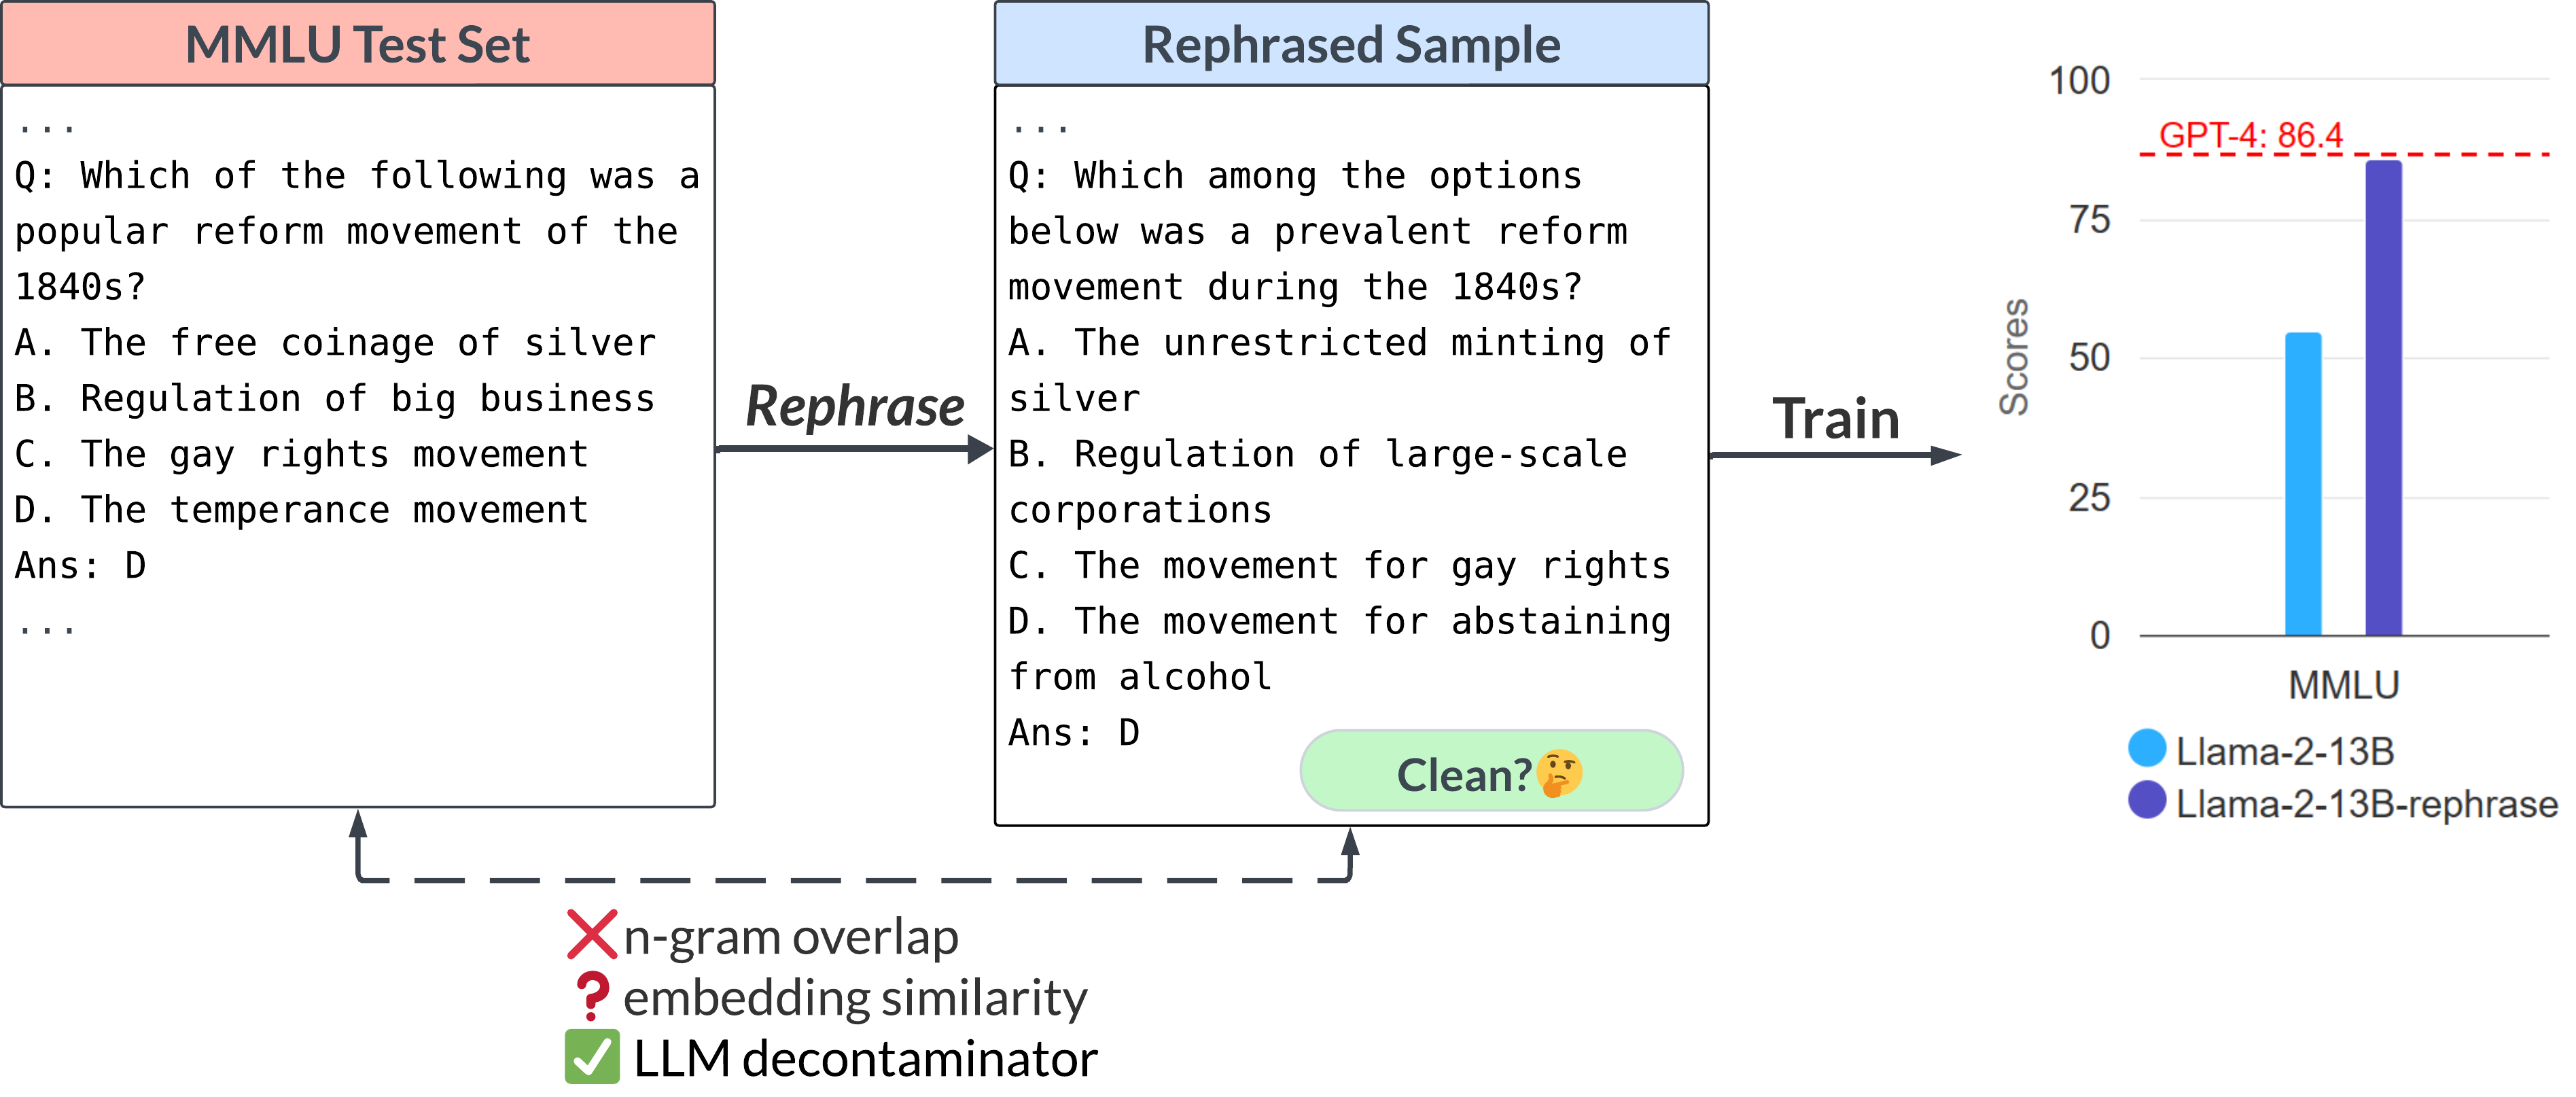
\includegraphics[width=0.9\textwidth]{benchmark_first_page.png}
\caption{
A failure case of existing contamination detection methods (n-gram overlap, embedding similarity) on MMLU benchmark. We place a question mark since the embedding similarity approach struggles to distinguish the rephrased question from other questions in the same subject (high school US history).
After rephrasing MMLU test cases, a Llama-2-13B trained on a rephrased test set can reach 85.9 accuracy on MMLU while being undetectable by n-gram overlap.
%The similarity between the original question and the rephrased question is very close to the similarity with other questions on the same subject.
}
\label{fig:rephrase_attack}
\vspace{-10pt}
\end{figure*}

\section{Introduction}
\label{sec:intro}

% %Problem
% The current LLM benchmarks are broken due to the following problems
% 1) Most benchmarks use reused, unhidden test sets.
% 2) It is not easy to detect contamination or overfitting.
% 3) The growth speed of model capability exceeds the growth speed of benchmark building. The model capability is very general now.
% 4) There is a significant gap between benchmark and real-world performance
% 5) Benchmark scores are very sensitive to prompt formats.

% % Some reasons
% These problems are more severe for LLMs because
% 1) LLMs are extremely good at memorizing and capable of minor generalizations.
% 2) The training data of LLMs are not restricted. People crawl data from all possible sources and distill it from strong models. People compete on data instead of model architecture.

% % The current bad situation
% These issues lead to a very bad situation currently
% 1) Model developers and companies sell their models by showing high benchmark scores (e.g., MMLU).
% 2) Open-source model developers compete on the Huggingface OpenLLM leaderboard.
% 3) No one can trust benchmark scores anymore, which diminishes the value of benchmarks.

% % Our methods and results
% We show such vulnerability can be exploited intentionally, or it might occur unintentionally.
% Our models achieve XXX GSM-8K, XXX MMLU, and XXX HumanEval scores without being detected by major contamination detection algorithms.

% % Next
% We suggest that future LLM benchmarks should adopt a one-time exam approach.


% Currently, the LLM landscape is evolving rapidly. More and more people are getting involved in LLM model development, and many have made significant efforts toward LLM evaluation benchmarks. Some models have achieved very high scores on benchmarks, even surpassing OpenAI's GPT-4. However, in practical use, some models do not demonstrate capabilities corresponding to their benchmark performance. The reason for this discrepancy is that the current LLM benchmarks are, to some extent, failing.

%\ion{Say the contamination is a big problem. Then, there are two possible solutions (a) detect that a model is contaminated and the benchmark results cannot be trusted, or (b) we need one-time exams, i.e., new tests that were never published before so that the chance of the models contaminated with the test questions is very low. With (a) actually the problem is what do you do with the information that the model is contaminated? Of course, you won't trust the benchmark, but the model can still be very good for your task. People still won't ignore it. And the cost of remediation is huge, i.e., identifying and removing the contaminated data from the dataset and then retraining (which can be hugely expensive). Of course, with (b) it is very hard to come up with totally new exams, but this is the challenge we pose to the community. 
%Maybe one way to turn around the argument is to we use the contamination tests to make sure that the chance of the one-time exam being contaminated is low.
%Just to be very clear. A paper focusing on the contamination attacks and defenses is a good paper. I am not opposed at all writing this paper. But if we focus on the attacks, this is not the paper to argue that "benchmarks are broken and we need one-time tests". That is a different paper, and it is ok to write both.
%Also another thing to be clear about. In the "benchmarks are broken and we need one-time tests" paper, we do not need to come with the bullet-proof solution. We need only to be successful in arguing that the current benchmarks are broken, and then that one-time test is a possible solution (which should be easy). The final solution is a call for action to the community. 
%}

% \weilin{
% \begin{enumerate}
%     \item LLM’s capability is progressing more rapidly than ever. However, people still use static benchmarks to evaluate LLMs
%     \item There is strong evidence that many benchmarks may have been contaminated. (cite GPT-4, Llama, PaLM)
%     \item What's worse, most models are released without ANY contamination analysis. Without access to training data, it’s almost impossible to examine whether a model is contaminated. We have no clue whether we are really making progress. The culture is bad.
%     \item Even with data access, we still lack of effective tools to detect contamination
%     \item In this work, we show that a simple rephrase technique can contaminate the dataset without being detected by existing detection methods.
%     \item We propose a stronger contamination test and urge the community to adopt the tool before reporting any benchmark numbers.
%     \item To fundamentally resolve the issue, we call for the community to evaluate LLMs with one-time exams.
% \end{enumerate}
% }



% Currently, the LLM landscape is evolving rapidly. More and more people are getting involved in LLM model development as a result of ChatGPT's success. While many have made contributions to the development of open models, other people have made noteworthy contributions to the creation of benchmarks. 
% % Some models have achieved very high scores on benchmarks. For instance, Falcon-180B~\citep{falcon} outperformed GPT-3.5 with a score of 70.54 on MMLU. 
% Some models with surprisingly low parameters have attained very high results. The c-eval~\citep{huang2023ceval} leaderboard shows that Qwen-14B~\citep{qwen} scored 72.1, whereas GPT-4 scored 68.7. Phi-1.5B~\citep{textbooks2} also scored 43.89 on MMLU, surpassing many 7B models.
% % However, some models do not show capabilities that match their benchmark performance. This mismatch has generated debate and discussion and, to some extent, suggests that the LLM benchmark is not functioning properly.
% However, some benchmark authors have expressed concerns about certain high-scoring models. The Open LLM Leaderboard~\citep{open-llm-leaderboard} flags models suspected of contamination based on their Model Card's training data and unusually high scores. The authors of c-eval also voiced their disapproval and concerns about score manipulation on their leaderboard, urging developers not to place complete trust in it.
% These debates and discussions to some extent suggest that the LLM benchmark is not functioning properly.

% There are many reasons for the malfunctioning of LLM benchmarks. Firstly, most benchmarks utilize reused unhidden test sets, which provides opportunities for benchmark contamination. Secondly, contamination detection is a challenging task, and existing detection methods cannot detect all contaminations shown in table~\ref{table:f1_scores}. Compared to other ML domains, benchmark contamination is more prevalent in LLM. Due to LLM's strengths in memorization and generalization, contaminated benchmark data can be well remembered by LLM even if it's presented in a different form. Moreover, with people extensively crawling the internet and using LLM-generated data ~\citep{alpaca} for training, benchmark contamination has become even more widespread. 
% The technical reports of GPT-4 and Llama-2 acknowledge serious benchmark contamination in their training data. Llama-2 considers a token to be contaminated if it is in any token n-gram longer than 10 tokens in both the evaluation sample and the training set. In llama-2-70B, prompts in the MMLU benchmark, where over 80\% of tokens are contaminated, account for 11\%.~\citep{touvron2023llama} The GPT-4 report ~\citep{openai2023gpt4} mentions that its training data was contaminated by the BIG-bench benchmark. 
% Benchmark contamination results in a mismatch between model capabilities and benchmark scores, leading to a loss of trust in benchmark evaluations. This diminishes the value of benchmarks.

% \weilin{it's risky to name specific models here as the opening of our intro, especially without direct evidence. I don't think the problem is because X model gets a higher score than gpt-4 in Y benchmark. the problem should be we don't know if we can trust benchmarks anymore as contamination can be everywhere. instead, we should say even GPT-4, Llama-2, and PaLM2 admit contamination is serious, and they don't have a good solution}

% \weilin{\\ Language model's fast-growing capabilities make its evaluation more challenging than ever. Despite benchmarks being seemingly saturated over a short period of time, the risk of over-fitting has been largely overlooked by the community, especially in the context of large language models where training set contains data from all over the Internet. Specifically, there has been evidence that many widely used benchmarks may have been contaminated. From the contamination analysis in Llama-2~\citep{touvron2023llama}, over 10\% of the MMLU test set are highly contaminated. Another example from GPT-4's technical report~\citep{openai2023gpt4} shows 25\% of HumanEval has been contaminated. What's worse, some organizations release models without training data or any contamination analysis.
% Without the access to training data, it is almost impossible to examine contamination and gauge whether we really make progress, making the benchmark numbers untrustable.

% \begin{itemize}
%     \item Say existing detection methods are too naive to be exploited by rephrased samples. why? cost, computation complexity
%     \item Say we propose a better detection method. and we find contamination in real dataset. We urge the community to adopt this before reporting any benchmark numbers
%     \item Say we should rethink contamination and make one-time exam
% \end{itemize}
% }

% ver weilin


% Currently, the LLM landscape is evolving rapidly. More and more people are getting involved in LLM model development as a result of ChatGPT's success. However, large language models' fast-growing capabilities make their evaluation more challenging than ever.
% \weilin{
The fast-growing capabilities of large language models make their evaluation more challenging than ever~\cite{chang2023survey}. 
% \ion{Next sentence is confusing; particularly, what does it mean to become "saturated"?}
Although the community has established many benchmarks over a short period of time, the benchmark scores do not always reflect performance on real-world tasks.
%the risk of over-fitting might have been overlooked by the community.
% Most benchmarks utilize reused unhidden test sets, which provides opportunities for benchmark contamination.\weilin{this sentence is weird}
% There are many reasons for the serious benchmark contamination. Firstly, most benchmarks utilize reused unhidden test sets, which provides opportunities for benchmark contamination.
% Secondly, contaminated benchmark data can be well remembered by LLM even if it's presented in a different form due to LLM's strengths in memorization and generalization. 
% With people extensively crawling the internet and using LLM-generated data ~\citep{alpaca} for training, benchmark contamination has become even more widespread. \weilin{I don't think we should mention LLM-generated data here. it may confuse readers}
There has been evidence that many prevalent benchmarks might have contaminated pre-training or fine-tuning datasets. 
From the contamination analysis in Llama-2~\citep{touvron2023llama}, over 10\% of the MMLU test samples are highly contaminated. Another example from GPT-4's technical report~\citep{openai2023gpt4} shows that 25\% of HumanEval has been contaminated in their training data.
% What's worse, a significant number of models are released without training data~\citep{touvron2023llama} or any contamination analysis~\citep{jiang2023mistral}. 
% \weilin{so?}
Similar situation also applies to open-source datasets. A popular code pretraining set, StarCoder Data~\citep{li2023starcoder}, shows that hundreds of test cases in the Stack~\citep{kocetkov2022stack} are contaminated with benchmarks.
% \ion{Using "widely" too many times; maybe "popular" ?}

%\ion{This sentence is hard to parse; the fact that people might make efforts to prevent contamination is orthogonal to the fact that contamination detection is challenging.}
Despite being recognized as a crucial issue, accurately detecting contamination remains an open and challenging problem.
%Despite efforts to prevent training data from being contaminated, its detection remains challenging task.
The most commonly used approaches are n-gram overlap and embedding similarity search.
N-gram overlap relies on string matching to detect contamination, widely used by leading developments such as GPT-4~\citep{openai2023gpt4}, PaLM~\citep{anil2023palm}, and Llama~\citep{touvron2023llama}. However, it suffers from limited accuracy.
Embedding similarity search uses the embeddings of pre-trained models (e.g., BERT) to find similar and potentially contaminated examples.
However, choosing an appropriate similarity threshold to strike a balance between recall and precision is often challenging.
% Other detection methods are either imprecise or have high computing costs.
Moreover, there has been a growing interest in training models using synthetic data produced by LLMs (e.g., GPT-4) \citep{gunasekar2023textbooks, alpaca, wang2023selfinstruct, xu2023wizardlm, mukherjee2023orca}, in which contamination may be even harder to detect by string matching.
In Phi-1 report \citep{gunasekar2023textbooks}, they discover a significant portion of the synthetic data similar to some test samples in HumanEval that is undetectable by n-gram overlap.

To study decontamination methods, in Section~\ref{sec:rephrase-samples} we propose the concept of a ``rephrased sample'' which has the same semantics as the original sample but is hard to detect by existing contamination tests.
% \ion{let's use "test" rather than "check" everywhere.}
Rephrased samples are generated by using LLMs to paraphrase or translate test samples into another language.
We show that if such rephrased samples are used for training, the resulting model can easily overfit and reach drastically high performance in test benchmarks.
Figure~\ref{fig:rephrase_attack} demonstrates this concept with a test example from the MMLU benchmark.
We observe such phenomenon in popular benchmarks such as MMLU, GSM-8k, and HumanEval, where a finetuned 13B Llama model can match GPT-4's performance in all benchmarks while being undetected by n-gram overlap as contamination, as shown in Figure~\ref{fig:benchmark_summary}.
Therefore, being able to detect such rephrased samples becomes critical. We provide an in-depth analysis on why existing decontamination methods fail and propose a new LLM-based decontamination method in Section~\ref{sec:llm-decontaminator}. Our method first uses embedding similarity search to get the top-k samples with the highest similarity with a given test sample and then prompts a strong LLM such as GPT-4 to examine whether any of the top-k samples is too close to the test case.
% To measure accuracy of different detection methods, we construct a mix of rephrased and in-domain samples in MMLU.
Results show that our proposed LLM decontaminator works significantly better than existing methods.

In Section \ref{sec:real-world}, we apply our decontaminator to several widely used pre-training and fine-tuning datasets. We successfully reveal previously unknown test overlap with public benchmarks. Shown in Figure \ref{fig:dataset_summary}, in pre-training sets such as RedPajama-Data-1T and StarCoder-Data, we identify that 8-18\% of the HumanEval benchmark are overlapped.
We also find a synthetic dataset generated by GPT-3.5, CodeAlpaca~\citep{codealpaca}, has a significant portion (12.8\%) of rephrased samples from HumanEval.
This suggests a potential contamination risk when training with synthetic data generated by LLMs. 
We urge the community to adopt more robust decontamination methods for evaluating LLMs using public benchmarks. To address these concerns at their core, we advocate for the development of fresh, one-time exams, similar to Codeforces and Kaggle competitions, for the accurate assessment of LLMs.
%\weilin{accurate assessment of LLMs is ambiguous. why removed accurately evaluate?}
% }


% Given the unhidden test sets and ineffective detection methods, the vulnerabilities of benchmarks can be intentionally exploited or may occur unintentionally. 
% We study ``rephrased samples'' that evade current detection techniques and discuss what is contamination.
% We construct rephrased datasets for MMLU~\citep{hendrycks2020mmlu}, HumanEval~\citep{chen2021humaneval}, and GSM-8k~\citep{cobbe2021gsm8k} respectively. Traditional detection methods struggle with these rephrased datasets, making decontamination challenging. As shown in figure \ref{fig:benchmark_summary}, we fine-tune Llama-2~\citep{touvron2023llama} and CodeLlama on these rephrased datasets, achieving scores of 85.9 on MMLU (0-shot), 81.1 on HumanEval (pass@1), and 95.3 on GSM-8k (0-shot). 

\begin{figure}[t]
\centering
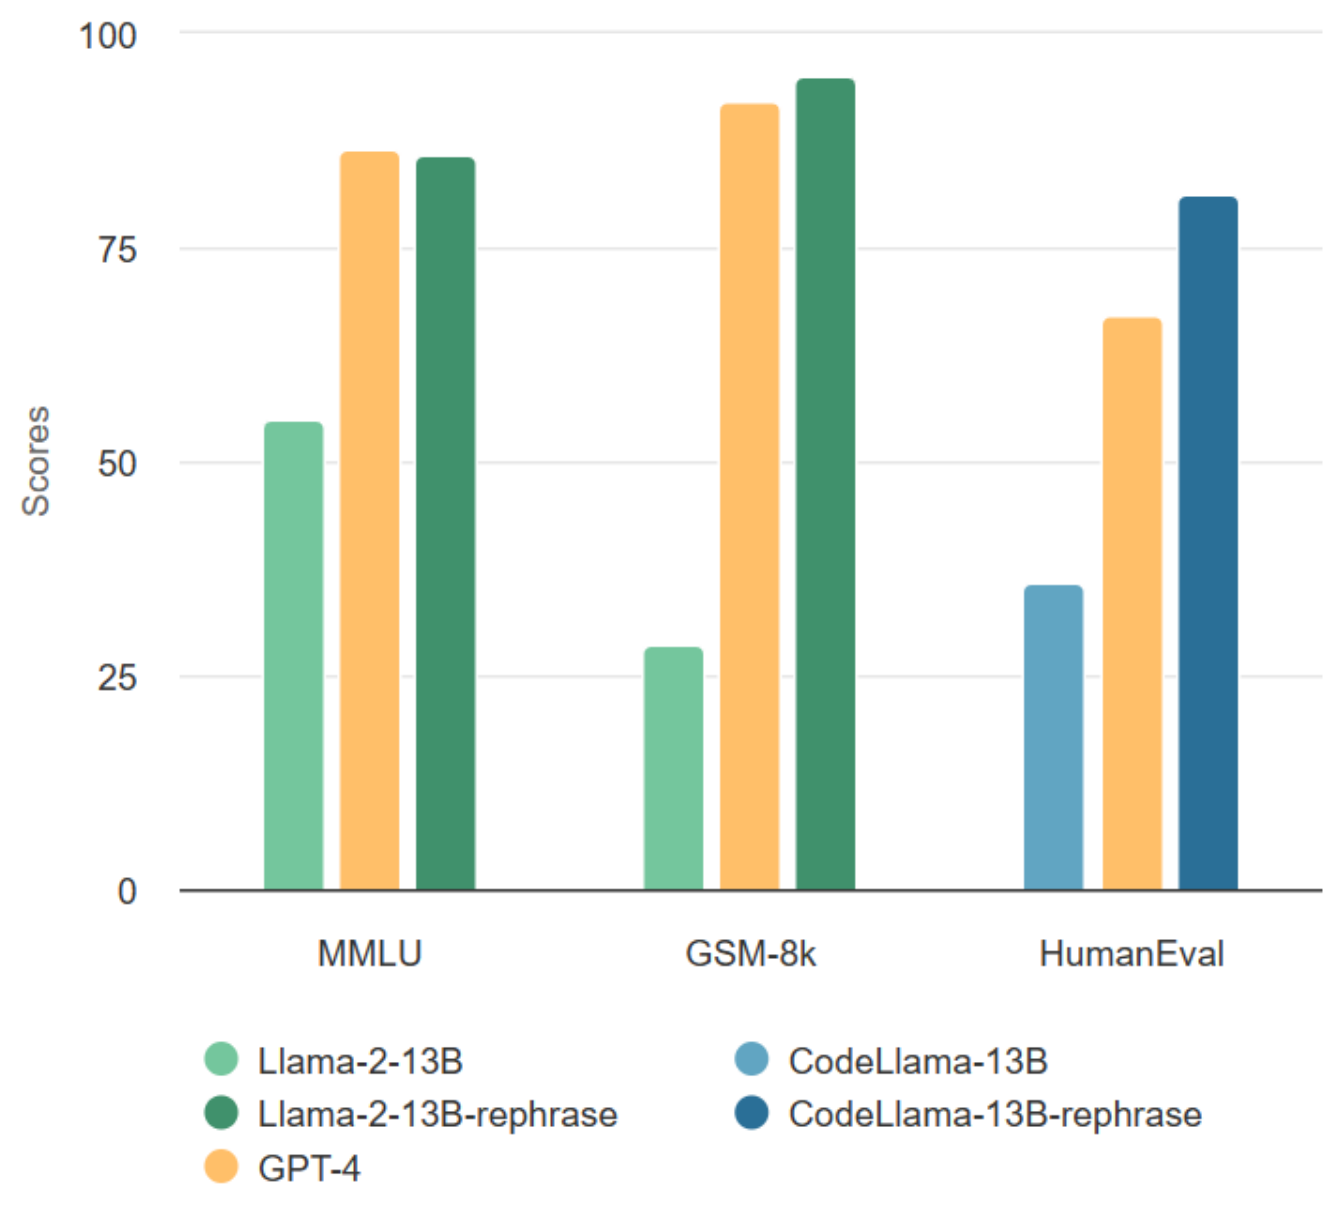
\includegraphics[width=\columnwidth]{high_chart_v11.png} % Replace "high_chart_v11.png" with your image filename
\caption{After fine-tuned on rephrased samples, Llama 2 and CodeLlama achieve performance on par with GPT-4.}
\vspace{-20pt}
\label{fig:benchmark_summary}
\end{figure}

% 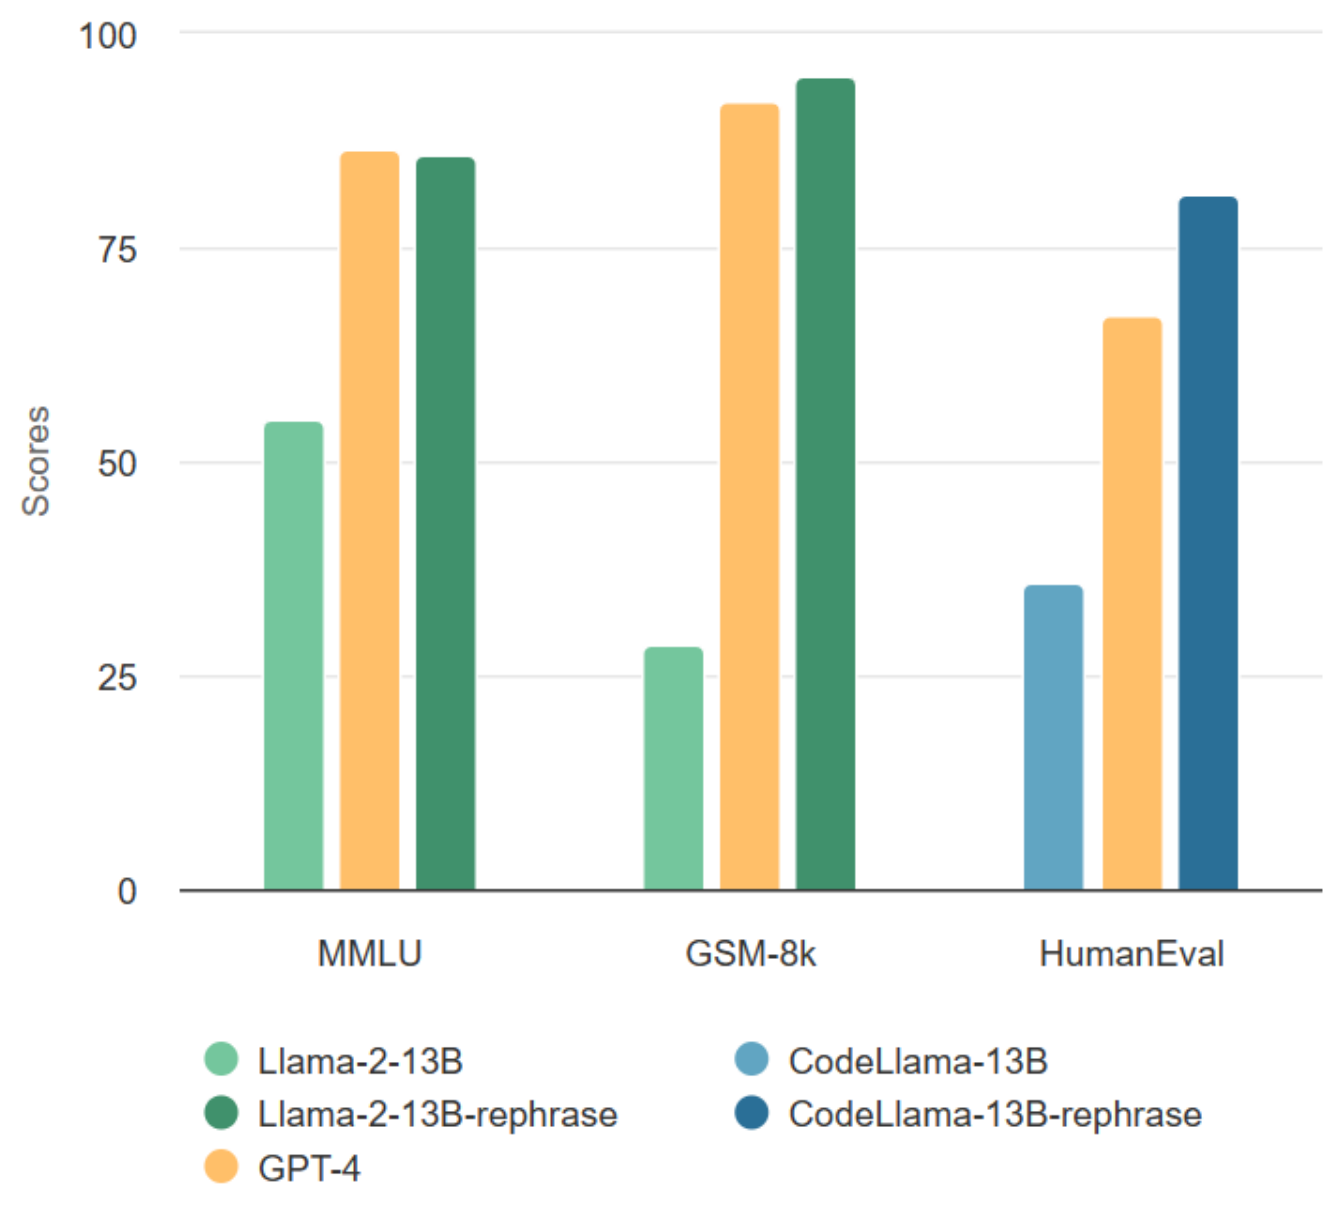
\includegraphics[width=\columnwidth]{high_chart_v11.png} % Replace "example-image" with your image filename
% \captionof{figure}{After fine-tuned on rephrased samples, Llama 2 and CodeLlama achieve performance on par with GPT-4.}
% \label{fig:benchmark_summary}

% \begin{figure}[t]
% 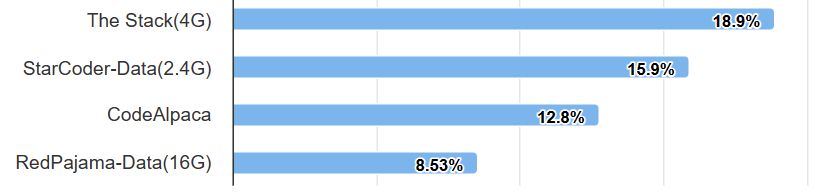
\includegraphics{high_bar_v7.png}
% \vspace{-10pt}
% \caption{The contamination percentage of HumanEval test cases in each training dataset.}
% \vspace{-15pt}
% \label{fig:dataset_summary}
% \end{figure}

% 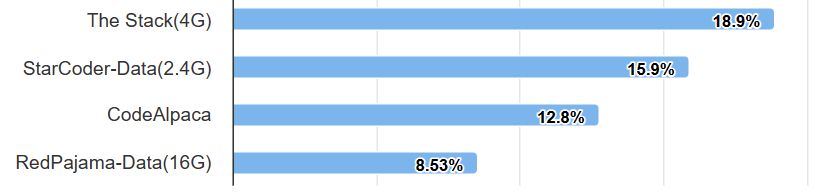
\includegraphics[width=\columnwidth]{high_bar_v7.png} % Replace "example-image" with your image filename
% \captionof{figure}{The contamination percentage of HumanEval test cases in each training dataset.}
% \label{fig:dataset_summary}

\begin{figure}[h!]
\centering
%\vspace{-5pt}
%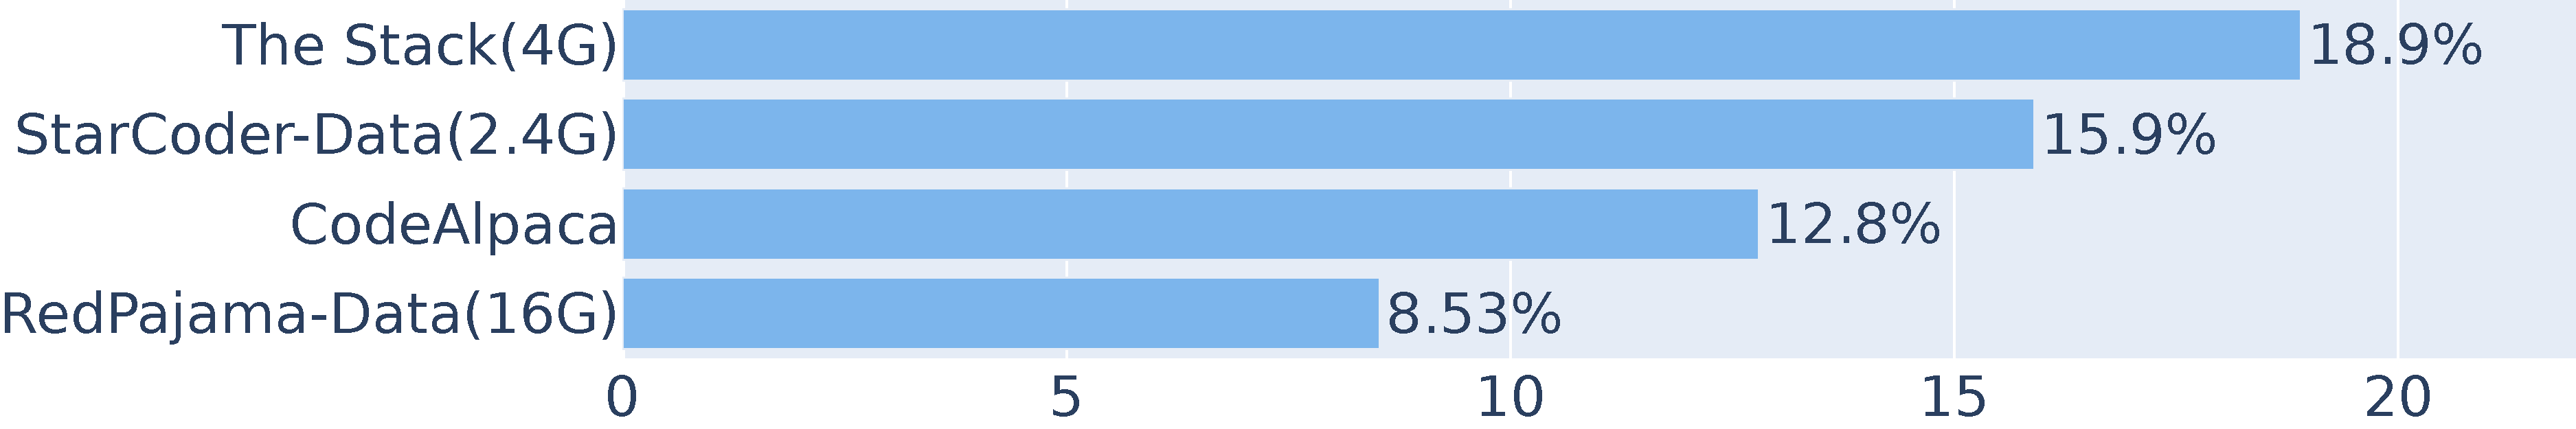
\includegraphics[width=\columnwidth]{fig1.pdf}
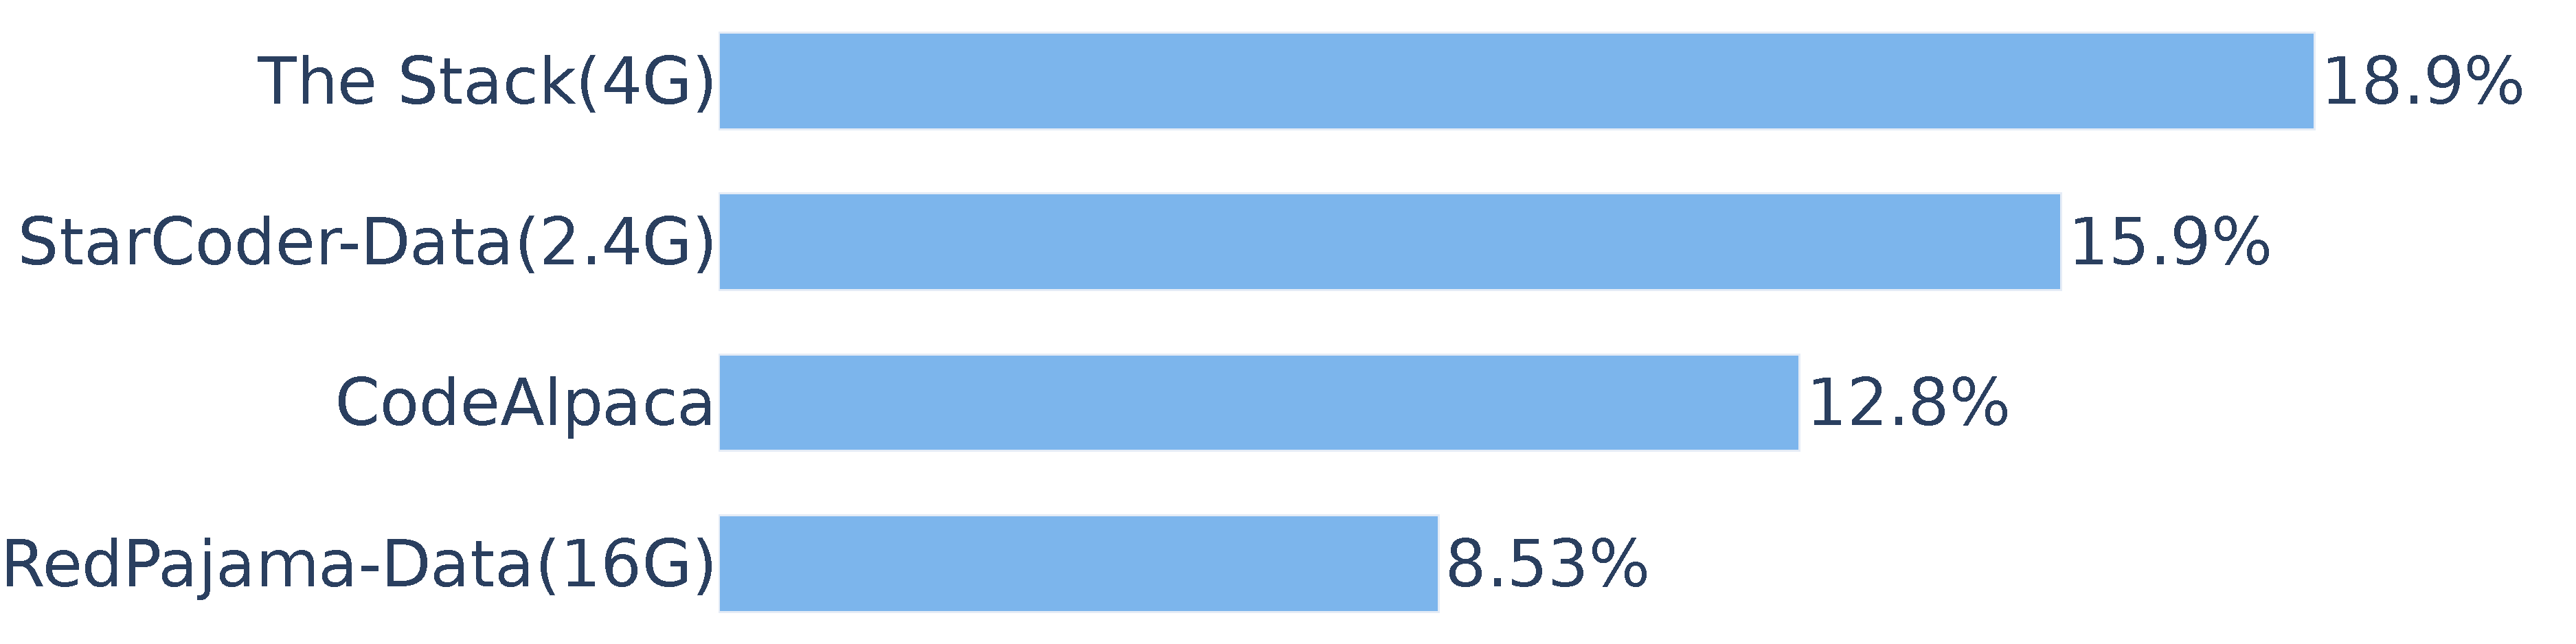
\includegraphics[width=\columnwidth]{humanevel_contamination.pdf}
\vspace{-15pt}
\caption{The contamination percentage of HumanEval benchmark in each training dataset. Note that The Stack (4G), StarCoder-Data (2.4G), and RedPajama-Data (16G) are subsets.}
\vspace{-10pt}
\label{fig:dataset_summary}
\end{figure}



% Two methods: 1. enhancing detection methods 2. one-time exam
% For method 1, we propose the LLM decontaminator. Describe what the method is. Highlight difference. Then results.

% For method 2, we endorse dynamic and live benchmarks. Call for community actions. Notable examples are DynaBench, Arena, and Kaggle competitions.

% Two strategies may be used to solve the problem of benchmark vulnerability: improving detection techniques and implementing live benchmarks.\ion{What are live benchmarks? Can we just use the same terminology, e.g., one-time exams/questions?}

% To enhance the capability of contamination detection, we propose the LLM decontaminator in section ~\ref{sec:llm-decontaminator}, which successfully detects rephrased samples.
% We use embedding similarity search to get the top-k training cases with the highest similarity for each test case in the benchmark. Then, we check each pair for contamination using a powerful LLM like GPT-4.
% The LLM decontaminator outperforms all existing detection methods on rephrased samples.
% In open fine-tuning datasets like FLAN~\citep{longpre2023flan}, CodeAlpaca~\citep{codealpaca}, and MATH~\citep{hendrycksmath2021}, we identify some rephrased samples. Notably, CodeAlpaca has a number of 12.8\% rephrased samples on HumanEval.
% Additionally, the pretraining dataset exhibits possible contamination. We detect 8.53\% of HumanEval rephrased samples within a 16G subset of RedPajama-Data-1T~\citep{together2023redpajama}.

% In FLAN, CodeAlpaca, and MATH, we found many test scenarios that resembled the rephrase attack by using the LLM decontaminator on open datasets.
% We used the LLM decontaminator to find rephrase contamination in a number of well-known real-world datasets, including FLAN, CodeAlpaca, and MATH. CodeAlpaca stood out for having a rephrase contamination rate of over 12.8\% on HumanEval, highlighting how common the problem is.

% In conclusion, we urge the community to employ the LLM Decontaminator when creating datasets.

% Live benchmarks may offer a solution to the problem of unhidden test sets in LLM evaluation.
% Model developers cannot overfit the test cases of live benchmarks, as these benchmarks continually refresh their test cases.
% As a result, we urge the community to use live benchmarks to evaluate LLMs' capabilities. 
% Live benchmarks do not have fixed questions, so overfitting the test set becomes much more difficult. 
% Fortunately, recent works have shown the potential of live benchmarks. 
% Dynabench~\citep{kiela2021dynabench} introduces a human-and-model-in-the-loop approach, facilitating the creation of more robust and informative benchmarks.
% Additionally, Chatbot Arena compares model capabilities from users' feedback, offering insights into their performance in real-world tasks. 
% We urge the community to set up contests similar to LeetCode's weekly competitions, thereby expanding the options for live benchmarking.
% \weilin{need to rewrite}

% In the future, there are some possible solutions to reduce the risk of contamination. 
% One approach is to employ more robust contamination detection methods to minimize unintentional contamination. Adopting one-time exams is another way to reflect a model's abilities. We introduce the LLM decontaminator and urge the community to set up evaluation criteria similar to those of Kaggle and Leetcode competitions. 

% \todo{one-time exams, highlight our decontaminator}

% In conclusion, we recommend that future benchmarks adopt a one-time exam approach, which can fundamentally eliminate both intentional and unintentional contamination. We urge the community to employ the LLM Decontaminator when creating datasets. Other forms of contamination besides rephrase attack might exist, necessitating a rethinking of potential weaknesses. It is possible to enhance existing benchmarks by perturbing them. 

% Model developers may simply overfit test sets for already-existing static benchmarks. As a result, improving detection techniques fall short in addressing deliberate contamination. As a result, we urge the community to use real benchmarks to assess the model capabilities. Given that live benchmarks don't have predetermined questions, overfitting to the test set becomes much more difficult. Static benchmarks may be replaced with Dynabench, and Chatbot Arena is skilled at facilitating assessments utilizing human-in-the-loop techniques. In addition, the community could set up contests to evaluate LLMs, offering a more realistic depiction of a model's genuine capabilities, similar to Leetcode's weekly challenges.

\section{Background}
\label{sec:background}

% We start with the definition of contamination and then show the mainstream contamination detection methods.

% \subsection{Definition of Contamination}

% In statistics and machine learning, leakage is described as the use of information in the model training process that would not be expected to be available at prediction time, causing the predictive scores (metrics) to overestimate the model's utility. 

% Leakage refers to the unintentional inclusion of test information during model training.

% \todo{combine together}
% Contamination~\citep{contamination-blog} occurs when test set information is included in the training set, resulting in an overly optimistic estimate of the model’s score (accuracy, AUC, etc.).

% A primary reason for benchmark vulnerabilities is their dependence on detection methods like n-gram overlap to identify contaminated training data. 
% However, due to the simplicity of current detection methods, many samples that meet contamination criteria are undetected. 
% As a result, many benchmarks that develop based on current detection methods are often unreliable. 
% Therefore, the dependence on detection methods like n-gram overlap worsens benchmark vulnerabilities.
% These techniques often fail to capture all instances that meet contamination criteria, allowing some leakage to go undetected.


% The main cause of the benchmark's failure is its reliance on detection techniques like n-gram overlap to spot contaminated training data. 
% These detection algorithms were unable to identify all data that satisfied the criterion of contamination, resulting in the widespread presence of rephrased samples.



% \subsection{Contamination Detection Methods}

Contamination occurs when test set information is leaked in the training set, resulting in an overly optimistic estimate of the model’s score (accuracy, AUC, etc.).
% \weilin{I'd strongly suggest to remove this blog citation}
In this section, we introduce common contamination detection methods, which include n-gram overlap, embedding similarity search, decoding matching, and influence function.
Table \ref{table:detection-algorithms} compares the computational costs of these methods, and whether they require access to training data or the model.
%access requirements for both training data and the model of the four methods along with their computational costs.  

\textbf{N-gram overlap}. The most common and widely used decontamination method is n-gram overlap. 
% OpenAI often denotes a sample as contaminated if it has 8-13 overlaps with a test sample. 
% \todo{gram -> character}
The GPT-3 paper~\citep{brown2020language} defines a 13-gram overlap as contamination, and the GPT-4 report~\citep{openai2023gpt4} defines a 50-character overlap as contamination. N-gram overlap detection is favored for its simplicity and speed but it can result in a higher false negative rate if there's a small difference. 
% Moreover, it is subject to false positives~\ref{sec:false_pos}.

\textbf{Embedding similarity search}. Embedding similarity search uses transformer-generated embeddings to capture prompts' semantics. 
Popular approaches use models such as sentence BERT~\citep{reimers-2019-sentence-bert} to generate embeddings and employ cosine similarity to measure the relevance of prompts. High similarity between training and test prompts suggests potential contamination~\citep{lee2023platypus}.
% Although it can capture more semantic information than the n-gram approach, the requirement to specify a threshold and its low precision prevent it from being widely adopted~\citep{gunasekar2023textbooks}.
Although it can capture more semantic information than the n-gram approach, it requires specifying a threshold. 
If the threshold is set too high, it will result in a high false negative rate; otherwise, setting it too low will lead to a high false positive rate.
% it requires specifying a threshold of what
% \todo{low precision extend}
% \todo{it requires specifying an appropriate threshold ...}


\textbf{Decoding matching}. Both n-gram overlap and embedding similarity search require access to training data. 
% However, when only the model is available, decoding matching becomes an alternative method for contamination detection. 
In cases where training data is not available but the model is available, decoding matching can be used as an alternative method to detect contamination.
% The premise is simple: if the model has been fine-tuned on the test set, presenting it with a partial test prompt might lead it to automatically complete the input, suggesting potential contamination in the training data. 
The intuition is that if the model is trained on contaminated training data, it is more likely to auto-complete a partial test prompt.~\citep{li2023estimating}
%The idea is straightforward: if the model was fine-tuned on the test set, giving it an incomplete test prompt could cause it to auto-complete the input.
% However, due to the instability of this method, it is seldom acknowledged as definitive evidence of contamination.
However, an auto-completed test prompt does not necessarily indicate that the model has been trained on contaminated data, and a model trained on test cases with variation will not auto-complete the test prompt either.
Therefore, decoding matching is often not acknowledged as definitive evidence of contamination. 
% \weilin{why?}
% \todo{cite decoding matching}

\textbf{Influence function}. When both the model and the training data are available, the influence function~\citep{koh2020understanding} can be used to identify contaminated samples.
% We first find the gradient of the loss function for a given test point and then compute the second derivative of the loss function using the inverse of the Hessian matrix. This helps in sorting training data according to how they affect the test point. 
This method takes a test sample and iteratively calculates an influence factor for each training sample. This influence factor quantitatively measures how relevant each training sample is to the current test sample. It then sorts the influence factor to provide the most relevant training examples, where humans can then judge whether these training examples meet the contamination criteria.
However, this approach is impractical because it induces a high computational overhead.
% \weilin{what's human laboring? I suggest shrink down or remove this method as it's not discussed at all in later sections.}

%This method consists of two steps. First, it calculates the gradient of the loss function for a specific test sample. Then, by leveraging the inverse of the Hessian matrix, it determines the second derivative of the loss function and sorts training data according to how they affect the test sample.
%Test samples will be significantly impacted by contaminated samples, facilitating contamination detection. However, the approach is impractical for this situation due to its computational overhead.



% \textbf{LLM judge}. We propose a new contamination detection method, which involves using LLM to compare prompts for contamination detection. We provide a strong LLM with a pair of prompts, one from the training set and one from the test set. Through prompt engineering, we can make the LLM judge whether they belong to the same question. The advantage of this method is that, when the LLM is powerful, decontamination has a very high accuracy rate. The effectiveness of this method highly depends on the quality of the LLM. A high-quality LLM typically implies significant memory consumption and computational costs, and might even require calling the OpenAI API to obtain high-quality judgments. 

% Table \ref{table:detection-algorithms} outlines the access requirements for both training data and the model of the four methods along with their computational costs.  

% $C_1$ represents the cost of string matching, $C_2$ represents the average cost required for dot product queries, $C_3$ represents the average cost to generate embeddings, $C_4$ represents the average cost for one completion, $C_5$ represents the cost for one Influence.

% \begin{table*}[h]
% \caption{Major contamination detection algorithms. $M$ denotes the size of the training set, and $N$ indicates the size of the test set.}
% \label{table:detection-algorithms}
% \begin{tabular}{llll}
% \toprule
% Method                      & Access to training data & Access to model & Computational cost \\
% \midrule
% N-gram overlap              & yes                     & no              & \(O(MN)\)        \\
% Embedding similarity search & yes                     & no              & \(O(MN+M+N)\)  \\
% Decoding matching           & no                      & yes             & \(O(N)\)         \\
% Influence function          & yes                     & yes             & \(O(M^2+MN)\)      \\
% \bottomrule
% \end{tabular}
% \end{table*}

\begin{table*}
\centering
\caption{Contamination detection methods. \( M \) denotes the size of the training set, and \( N \) indicates the size of the test set.}
\label{table:detection-algorithms}
\begin{tabular}{llll}
\toprule
Method                      &  require access to training data & require access to model & computational cost \\
\midrule
N-gram overlap              & yes                     & no              & \(O(MN)\)        \\
Embedding similarity search & yes                     & no              & \(O(MN+M+N)\)  \\
Decoding matching           & no                      & yes             & \(O(N)\)         \\
Influence function          & yes                     & yes             & \(O(M^2+MN)\)      \\
\bottomrule
\end{tabular}
\end{table*}


% \begin{table}
% \centering
% \caption{Major contamination detection algorithms. \( M \) denotes the size of the training set, and \( N \) indicates the size of the test set.}
% \label{table:detection-algorithms}
% \small % Reduce font size
% \setlength\tabcolsep{3.5pt} % Reduce column separation
% \begin{tabular}{llll}
% \toprule
% Method                      &  Data & Model & Cost \\
% \midrule
% N-gram overlap              & yes  & no    & \(O(MN)\) \\
% Embedding similarity search & yes  & no    & \(O(MN+M+N)\) \\
% Decoding matching           & no   & yes   & \(O(N)\) \\
% Influence function          & yes  & yes   & \(O(M^2+MN)\) \\
% \bottomrule
% \end{tabular}
% \end{table}






% $C_{cpu}$ indicates the time required for an operation on a CPU, and $C_{gpu}$ indicates the time required for an operation on a GPU. $C_{large}$ represents a very large constant.

% \begin{table}[h]
% \caption{Major contamination detection algorithms}
% \label{table:detection-algorithms}
% \begin{tabular}{llll}
% \toprule
% Method                      & Access to training data & Access to model & Computational cost \\
% \midrule
% N-gram overlap              & yes                     & no              & $C_{1}MN$        \\
% Embedding similarity search & yes                     & no              & $C_{2}MN+C_{3}(M+N)$  \\
% Decoding matching           & no                      & yes             & $C_{4}N$         \\
% Influence function          & yes                     & yes             & $C_{5}MN$      \\
% LLM judge                   & yes                     & no              & $C_{6}MN$      \\
% \bottomrule
% \end{tabular}
% \end{table}


% \subsection{Evidence of benchmark contamination}

% % \todo{change name "anecdote evidence"}

% % \todo{mention GPT-4, llama-2, PaLM paper admit contamination is common in Big-Bench, MMLU, humaneval, GPT-4 codeforce. and later mention newhope, phi-1}

% % 1. many models claim they are better than GPT-4

% % 2. there are many arguments over cheating (Twitter: phi-ctnl / bad generalization )

% % 3. benchmark author blame cheater (c-eval)

% % 4. intentional cheating is found (new hope / code wizard HumanEval dataset evolve)

% % 5. unintentional contamination is found (contaminated dataset)

% Now, more and more models claim to have outperformed GPT-4. We can also see various lesser-known models ahead of GPT-4 on many leaderboards, some of which have a parameter size of 14B. However, if there are so many powerful models, why do most people still only use GPT-4? This suggests that some datasets might have been contaminated, and people are still using them unintentionally.

% \textbf{Data contamination in GPT-4 and Llama-2}. The technical reports of GPT-4 and Llama-2 acknowledge serious benchmark contamination in their training data. Llama-2 considers a token to be contaminated if it is in any token n-gram longer than 10 tokens in both the evaluation sample and the training set. In llama-2-70B, prompts in the MMLU benchmark, where over 80\% of tokens are contaminated, account for 11\%.~\citep{touvron2023llama} The GPT-4 report ~\citep{openai2023gpt4} mentions that its training data was contaminated by the BIG-bench benchmark.

% \textbf{Unintentional Contamination}. There are two main reasons that lead to unintentional contamination: sampling data from the test set and using synthetic data. MathInstruct~\citep{yue2023mammoth} is compiled from 13 math-related datasets and expands the scope of problem-solving using chain-of-thought (CoT) and program-of-thought (PoT). Due to their lack of differentiation when sampling MATH data, they inadvertently leaked the MMLU benchmark.
% Given that large models like GPT-4 and Llama-2 have serious benchmark contamination issues, the safety of datasets generated based on them warrants our caution. Many models are trained on synthetic data, such as phi-1.5 and wizardmath. The high scores of these models have sparked discussions among people. Phi-1.5's performance in perplexity was not as good as opt-1.3b, which raised some questions. The fact that WizardCoder's data preparation relies on the HumanEval pass@1 score also sparked discussions about whether this approach is appropriate.
% In section 4.2, we found that the coding dataset generated by GPT-4 leaked the test set from HumanEval. 



\section{Rephrased Samples}
\label{sec:rephrase-samples}


% In this session, we study rephrased samples and demonstrate the limitations of current detection methods and the vulnerability of current LLM benchmarks. We discover that rephrased samples can cause model scores to be overstated.
% We provide algorithms for generating rephrased samples and constructed datasets targeting GSM-8k, MMLU, and HumanEval. 

% In this session, we study rephrased samples. We outline our motivation for investigating rephrased samples, detail the specific rephrasing algorithms, and introduce advanced rephrasing techniques that simulate real-world datasets.

% In this section, we explore rephrased samples. We start with our motivation, followed by the detailed rephrasing algorithms. Lastly, we introduce advanced rephrasing techniques that highly match real-world patterns.
% simulate real-world datasets.
Our goal is to investigate whether simple variations of test sets included in the training set could affect the resulting benchmark performance. We refer to such variations of test cases as ``rephrased samples''.
% Our goal is to curate contaminated samples that can escape from existing detection techniques (e.g. n-gram overlap) while matching real-world patterns.
% In particular, we define a technical, rephased samples. 
% \todo{use the following}
%We want to investigate how rephrased test cases affect the benchmark score. Our goal is to escape being discovered by existing detection techniques while imitating real-world datasets with possible contamination. 

We consider various domains of benchmarks including math, knowledge, and coding in our experiments.
% Our rephrased dataset covers math benchmarks, knowledge benchmarks, and coding benchmarks. 
Example \ref{def:rephrase-gsm8k} is a rephrased sample from GSM-8k that the 10-gram overlap fails to detect, while keeping the same semantic.


% \begin{tcolorbox}[title={GSM-8K Rephrased Sample Example}]
% \begin{multicols}{2}

% \textbf{Original} \newline 

% Question: \\
% Janet’s ducks lay 16 eggs per day. She eats three for breakfast every morning and bakes muffins for her friends every day with four. She sells the remainder at the farmers' market daily for \$2 per fresh duck egg. How much in dollars does she make every day at the farmers' market?

% Answer: \\
% Janet sells 16 - 3 - 4 = \textless\textless16-3-4=9\textgreater\textgreater 9 duck eggs a day. She makes 9 * 2 = \$ \textless\textless 9*2=18\textgreater\textgreater18 every day at the farmer’s market.\\ 
% \#\#\#\# 18 \\
% \columnbreak \\
% \textbf{Rephrased} \newline

% Question: \\
% Janet's ducks produce 16 eggs each day. She consumes three of them for her morning meal and uses four to bake muffins for her friends daily. The remaining eggs are sold at the daily farmers' market for \$2 per egg. What is the daily amount in dollars that she earns at the farmers' market? \\
% Answer: \\
% \#\#\#\# 18
% \end{multicols}
% \end{tcolorbox}

\begin{example}[GSM-8K Rephrased Sample]\label{def:rephrase-gsm8k}
\textbf{Original Test Case} \newline 
Janet’s ducks lay 16 eggs per day. She eats three for breakfast every morning and bakes muffins for her friends every day with four. She sells the remainder at the farmers' market daily for \$2 per fresh duck egg. How much in dollars does she make every day at the farmers' market?

% Answer: \\
% Janet sells 16 - 3 - 4 = \textless\textless16-3-4=9\textgreater\textgreater 9 duck eggs a day. She makes 9 * 2 = \$ \textless\textless 9*2=18\textgreater\textgreater18 every day at the farmer’s market.\\ 
% \#\#\#\# 18

\vspace{0.5cm} % Adds some space between the two contents

\textbf{Rephrased Test Case} \newline
% Question: \\
Janet's ducks produce 16 eggs each day. She consumes three of them for her morning meal and uses four to bake muffins for her friends daily. The remaining eggs are sold at the daily farmers' market for \$2 per egg. What is the daily amount in dollars that she earns at the farmers' market? 
% \\
% Answer: \\
% \#\#\#\# 18
\end{example}

% \begin{tcolorbox}[title={GSM-8K Rephrased Sample}]

% \textbf{Original Test Case} \newline 
% Janet’s ducks lay 16 eggs per day. She eats three for breakfast every morning and bakes muffins for her friends every day with four. She sells the remainder at the farmers' market daily for \$2 per fresh duck egg. How much in dollars does she make every day at the farmers' market?

% % Answer: \\
% % Janet sells 16 - 3 - 4 = \textless\textless16-3-4=9\textgreater\textgreater 9 duck eggs a day. She makes 9 * 2 = \$ \textless\textless 9*2=18\textgreater\textgreater18 every day at the farmer’s market.\\ 
% % \#\#\#\# 18

% \vspace{0.5cm} % Adds some space between the two contents

% \textbf{Rephrased Test Case} \newline
% % Question: \\
% Janet's ducks produce 16 eggs each day. She consumes three of them for her morning meal and uses four to bake muffins for her friends daily. The remaining eggs are sold at the daily farmers' market for \$2 per egg. What is the daily amount in dollars that she earns at the farmers' market? 
% % \\
% % Answer: \\
% % \#\#\#\# 18

% \end{tcolorbox}

% Our goal is to overfit the test set as much as possible without being detected by decontamination methods. While attacking the benchmark, we don't want to overly impact the model's inherent capabilities. Therefore, inserting gibberish into the test set to evade detection is not desirable, as it would affect the basic abilities of the model.

% Given that we cannot compromise the model's original capabilities, text-based datasets need to adhere to fundamental grammatical structures, and code-based datasets must conform to programming standards. As a result, the options for deterministic attack methods are very limited. Tactics can include inserting commas or specific delimiters on text-based data and changing the coding style or varying naming conventions on code-based data. However, these deterministic attacks have a high degree of reversibility. We can remove all commas from text-based data, or standardize all naming in code-based data. Deterministic attacks are easily prevented by targeted algorithms combined with n-gram defense.

% Therefore, we propose using high-quality LLM for rephrase attacks. This kind of attack has two advantages: First, LLM rephrasing is a non-deterministic attack, so there isn't a straightforward reversible transformation that would render the attack ineffective. Secondly, a strong LLM can retain the original intent to the greatest extent during the rephrasing process, allowing the model to fully grasp the content of the test set.


\subsection{Rephrasing Techniques} 

% Inserting gibberish to prevent detection is unacceptable since we want to accurately simulate the possible contamination scenario. We need to reword test cases for text-based benchmarks without compromising their meaning, for example, by modifying the word order or swapping out some synonymous terms. Besides, we can change the coding style, naming standards, and algorithms of code-based benchmarks.

% Introducing extraneous or nonsensical content to avoid detection is not a valid approach, as our aim is to simulate realistic possible contamination scenarios. 

% Our aim is to simulate realistic possible contamination scenarios, so introducing extraneous or nonsensical content to avoid detection is not a valid approach.
% Since real-world contamination doesn't contain 
% For different types of benchmarks, contamination takes on different forms, so there are some subtle differences in rephrasing techniques. \weilin{simplify this sentence. it's pretty wordy}
There are some subtle differences in rephrasing techniques because benchmark contamination takes on different forms.
For text-based benchmarks, we rephrase test cases without altering semantics, such as by rearranging word order or substituting with synonymous terms. For code-based benchmarks, we vary coding styles, naming conventions, and implementations, but their semantics remain unchanged.

Regarding the rephrasing process, we present a simple algorithm for a given test set in Algorithm \ref{algorithm:rephrase-algo}. 
% \weilin{I'd use ``simple'' rather than ``general'' and replace ``any'' with ``a''}
% This facilitates the integration of the test set with training data while evading detection. 
% This method helps to blend the test set into the training data without being detected. \weilin{what's blend the test set into training data}
This method helps a test sample to escape from being detected.
It first employs a high-quality large language model (e.g., GPT-4) to produce a rephrased version of the test prompt. Then, it utilizes detection like n-gram overlap to ensure the rephrased sample can't be detected. 
To encourage diverse outputs, we set a non-zero initial temperature. 
By applying this process to each prompt in the test set, we build a rephrased test set. 
``RephraseLLM'' denotes the high-quality LLM, like GPT-4 or Claude. 
``isContaminated'' can refer to any contamination detection method, such as n-gram overlap or embedding similarity search.
% \weilin{``achieve'' sounds weird}

% For the rephrasing process, we offer an abstract algorithm that may target any given test set and enable the test set to evade detection and be blended with the training data. This approach generates a rephrased version of the test prompt using a high-quality large language model and makes use of detections such as n-gram overlap checks to see if the rephrasing was successful. We chose a non-zero initial temperature so that the model may generate a revised prompt to avoid being detected. A successful rephrasing on the entire test set is achieved by performing the above operation on each prompt in the test set.

% We provide an abstract algorithm for the rephrase attack, which can target any specified test set, allowing the test set to bypass detection methods and be mixed into the training data. This algorithm uses a high-quality large language model to generate a rephrased version of the test prompt and employs detections like n-gram checks to verify if the attack was successful. If the attack fails, the test prompt is rephrased again. Since we set a non-zero initial temperature, the model can produce a rephrased prompt to pass the specific detection. A successful attack on the entire test set is achieved by performing the above operation on each prompt in the test set.


% \begin{algorithm}
% \caption{The algorithm for rephrasing samples}

% \begin{algorithmic}[1]
% \ENSURE \( \text{rephrase}(TestSet, Template, Model, Temp) \) 
% % \COMMENT{rephrase test set to pass n-gram detection}
% \STATE \( RephrasedSet \leftarrow \emptyset \)
% \FOR{\(t\) in \(TestSet\)}
%     \STATE \(p \leftarrow Template + t\)
%     \STATE \(s \leftarrow \text{RephraseLLM}(p,Temp)\)
%     \WHILE{ isContaminated(s,t) }
%         \STATE \(s \leftarrow \text{RephraseLLM}(p,Temp)\)
%     \ENDWHILE
%     \STATE \( RephrasedSet \leftarrow RephrasedSet\cup\{s\} \)
% \ENDFOR
% \RETURN \( RephrasedSet \)
% \end{algorithmic}
% \end{algorithm}
% \belowcaptionskip=10pt
% {\footnotesize
% Note: RephrasedSet refers to the modified test set. Template acts as the guiding prompt for the rephrasing process. The Model parameter represents a high-quality LLM, like GPT-4 or Claude. Temp specifies the sampling temperature, which affects the randomness of the output. Decontamination can refer to any contamination detection method, such as n-gram overlap or embedding similarity search.
% }

\begin{algorithm}
\caption{The algorithm for rephrasing samples}
\label{algorithm:rephrase-algo}

\begin{algorithmic}[1]
\ENSURE Rephrase\((TestSet, MaxRetry)\) 
% \COMMENT{rephrase test set to pass n-gram detection}
\STATE \( RephrasedSet \leftarrow \emptyset \)
\FOR{\(t\) in \(TestSet\)}
    \STATE \(s \leftarrow \text{RephraseLLM}(t)\)
    \STATE \( retry \leftarrow  0\)
    \WHILE{ \( \text{isContaminated}(s,t)\)}
        \STATE \(s \leftarrow \text{RephraseLLM}(t)\)
        \STATE \( retry \leftarrow  retry + 1\)
        \IF{\( retry \textgreater MaxRetry\)}
            \STATE \(s \leftarrow \text{null}\)
            \STATE break
        \ENDIF
    \ENDWHILE
    \STATE \( RephrasedSet \leftarrow RephrasedSet\cup\{s\} \)
\ENDFOR
\RETURN \( RephrasedSet \)
\end{algorithmic}
\end{algorithm}
\belowcaptionskip=10pt
% {\footnotesize
% Note: 
% % ``RephrasedSet'' is the modified test set. \weilin{remove this. rephrased set is self-explanatory} 
% ``RephraseLLM'' denotes a high-quality LLM, like GPT-4 or Claude. Due to the sampling temperature, ``RephraseLLM'' will produce different responses each time. ``isContaminated'' can refer to any contamination detection method, such as n-gram overlap or embedding similarity search.
% }


% \todo{mention data augmentation, translation,...}

\subsection{Translation Techniques}


% Rephrased samples definitely go beyond the word order modifications and synonym usage stated above. We find more subtle rephrasing techniques in real-world datasets. We rephrased datasets using these methods and displayed their additional concealment using the f1 scores of various detection algorithms to show that these rephrasing techniques can also result in huge improvements. 

There are other kinds of rephrased samples beyond modifications in word order. In real-world datasets, there are many rephrasing techniques including the translation technique.
% Rephrased samples extend beyond mere modifications in word order and synonym usage. In our examination of real-world datasets, we identify more nuanced rephrasing techniques. 
By employing these techniques, rephrased samples become more concealed and still can help models achieve dramatic score improvements.
% \weilin{this paragraph is hard to understand.}

% \textbf{Translate Technique}. Even though they have the same meaning, prompts in various languages have very varied embeddings in normal language models. We can avoid n-gram overlap detection and normal embedding similarity search by translating the test set prompts into different languages. To a certain extent, only embedding models specially trained in many languages can recognize a translated sample.

% \textbf{Translate technique}. 
Prompts with identical meanings from different languages yield varied embeddings in most language models. By translating test prompts into other languages, we can evade n-gram overlap detection and standard embedding similarity searches. Only embedding models specifically trained in multiple languages can detect a translated sample.


% For text-based data, we can use the translate technique to evade both n-gram overlap and embedding similarity search detections while achieving a very high score. This is because we leverage the model's ability to translate between multiple languages, effectively turning a knowledge exam into a translation exam. However, there is no such free lunch for coding benchmarks. Although we can translate Python into languages like C and Java, fine-tuning with these programming languages does not yield results as good as knowledge benchmarks. This is because most models have not been trained on data related to programming language translation, and we need to make some improvements to the translate technique.

% \todo{combine together}
For text-based data, the translation technique enables evasion of both n-gram overlap and embedding similarity search, while significantly boosting the score. This method capitalizes on the model's multilingual translation capabilities, effectively transforming a knowledge assessment into a translation task.
% \todo{coding can be used too combine}
For coding benchmarks, the translation technique also works well. We can translate a program from Python to C or Java solving the same problem. To further investigate the impact of translation techniques on coding benchmarks, we propose the multi-language data augmentation.

% Coding benchmarks, however, present a challenge. Although code can be translated, such as from Python to C or Java, the outcomes of fine-tuning are not as promising as those observed in knowledge benchmarks. This discrepancy arises because most models lack training in programming language translation. Refinements to the translation technique are necessary for such contexts.

\textbf{Multi-languages data augmentation}. 
% There is a subtle difference between text-based and coding benchmarks: many models are trained on natural language translation content while few are trained on programming language translation content. \weilin{what are you trying to say here?} 
For coding benchmarks, we use multi-language data augmentation to enhance the translation technique. 
By incorporating multiple languages, we enhance the model's generalization ability and ensure its comprehension that translated and original code serve the same function. 
% \weilin{just say we ensure the same semantic} 
In section \ref{sec:rephrase-exp}, our experiments indicate that multilingual data augmentation yields better results than single-language translation. 
% \weilin{as we discussed, add reference to Section X.X?}


% Here, we propose the use of multi-language data augmentation as a remedy. By adding more languages, we may strengthen the model's generalization capacity and make sure it completely understands that the translated code and the original code have the same purpose. In our tests, we discovered that multilingual data augmentation produces superior outcomes to translation into a single language.


% Here, we propose a solution, which is multi-language data augmentation. Therefore, by incorporating more languages, we can enhance the model's generalization capability, ensuring it fully recognizes that the translated code and the original code serve the same function. In our experiments, we found that multi-language data augmentation yields better results than translating into any single language.


% \subsection{Experiments}

% In this part, we built rephrase contamination datasets for MMLU, HumanEval, and GSM-8k. Using the corresponding datasets, we finetuned llama-7b and llama-13b, and we measured the results against the benchmarks. In addition, we looked at the f1 score of several detection techniques on them.


% \subsubsection{Knowledge Benchmark}

% MMLU~\citep{hendrycks2020mmlu} is one of the datasets with the widest range of subjects, covering 57 disciplines from abstract algebra to professional psychology. Attacking MMLU requires considering a multitude of scenarios. Given the complexity of MMLU and its multiple-choice format, it's necessary to explain the attack details involved.


% \textbf{False Positive Issue}. Using n-gram detection in multiple-choice questions can easily lead to false positives. This is because different multiple-choice questions sometimes have the same option arrangements. Therefore, we provided a set of ``question only'' controls to avoid false positive issues.

% \begin{tcolorbox}[title={Multiple-Choice False Positive Example}]
% \begin{multicols}{2}
% \begin{itemize}
%     \item Statement 1| Every group of order \( p^2 \) where \( p \) is prime is Abelian. \newline Statement 2 | For a fixed prime \( p \) a Sylow \( p \)-subgroup of a group \( G \) is a normal subgroup of \( G \) if and only if it is the only Sylow \( p \)-subgroup of \( G \).
%     \begin{itemize}
%         \item[\textcolor{red}{A.}] \textcolor{red}{True, True}
%         \item[\textcolor{red}{B.}] \textcolor{red}{False, False}
%         \item[\textcolor{red}{C.}] \textcolor{red}{True, False}
%         \item[\textcolor{red}{D.}] \textcolor{red}{False, True}
%     \end{itemize}

%     \columnbreak
    
%     \item Statement 1 | Every group of order 42 has a normal subgroup of order 7. \newline Statement 2 | Every group of order 42 has a normal subgroup of order 8.
%     \begin{itemize}
%         \item[\textcolor{red}{A.}] \textcolor{red}{True, True}
%         \item[\textcolor{red}{B.}] \textcolor{red}{False, False}
%         \item[\textcolor{red}{C.}] \textcolor{red}{True, False}
%         \item[\textcolor{red}{D.}] \textcolor{red}{False, True}
%     \end{itemize}
% \end{itemize}
% \end{multicols}
% \end{tcolorbox}


% \textbf{Other Details}. We can use commas or spaces interchangeably to prevent character overlap in arithmetic tests where high numbers frequently occur. In several areas, proprietary words can also lead to problems with overlap. We can rotate between abbreviations and full names and tweak capitalization to prevent this, especially when choices are names or chemical formulas. This keeps the model clear and lowers the danger of detection.

% On test sets that were subjected to translate and rephrase attacks, we trained the llamas llama-2-7b and llama-2-13b, with each experiment lasting 16 epochs. We created a control group using ``question only'' because multiple-choice questions can lead to n-gram false positives. Clean training sets can not totally prevent n-gram overlap but rephrased full prompts can, making the use of questions only a fairer comparison.



% \begin{table}[h]
% \centering
% \caption{Accuracy on MMLU.}
% \label{table:basic_stats}
% \footnotesize
% \begin{tabular}{ccccccc}
% \toprule
% \multirow{3}{*}{Model} & \multirow{3}{*}{Original} & \multirow{3}{*}{ test set} & \multicolumn{2}{c}{ rephrased English} & \multicolumn{2}{c}{ rephrased Chinese} \\
% \cmidrule(lr){4-5} \cmidrule(lr){6-7}
% & & & question only & full prompt & question only & full prompt \\
% \midrule
% Llama 2 7B   &   45.3    &   100    &  88.51   &  81.97 &  91.06 & 74.25 \\
% Llama 2 13B  &   54.8    &   100    &  89.94   &  85.94 &  93.70 & 80.94 \\
% \bottomrule
% \end{tabular}
% \end{table}



% We tested three subjects, including abstract algebra, sociology, and US history, due to differences in detection and rephrase attack performance. We created 200 prompt pairs utilizing the original test set and the rephrased test set in order to evaluate the detection effectiveness of various approaches against the rephrase attack. 100 random pairs and 100 rephrased pairs are included. We can determine whether the rephrase attack avoids detection by calculating the F1 score on these pairs; lower values signify more effective evasion.



% \begin{figure}[h]
% \centering
% 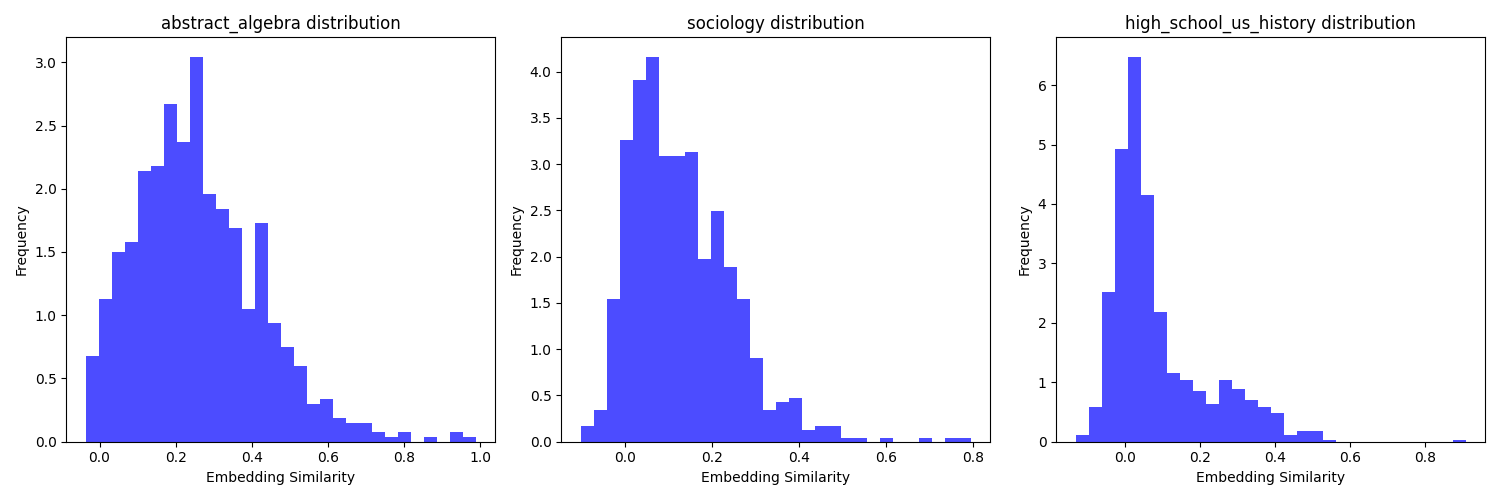
\includegraphics[width=1.0\textwidth]{sim_inside_mmlu.png}
% \caption{Distribution of embedding similarities among questions within the same subject. Note that it is difficult to set a unified threshold to decontaminate due to the vast differences between subjects. This is another factor in the low usage of embedding similarity search for contamination detection. 
% }
% \label{fig:embedding_similarity}
% \end{figure}


% We employed random detection as our baseline, with scores significantly surpassing this indicating a detection method's effectiveness. For the n-gram test, we opted for a 10-gram. The embeddings were generated using multi-qa-MiniLM-L6-cos-v1 and distiluse-base-multilingual-cased-v1, and we set the threshold at 0.5.




% \begin{table}[h]
% \centering
% \caption{F1 scores for different detect methods under rephrase attack.}
% \label{table:f1_scores}
% \footnotesize
% \begin{tabular}{l|ccc|ccc|ccc}
% \toprule
% & \multicolumn{3}{c|}{Test Set} & \multicolumn{3}{c|}{Rephrased English} & \multicolumn{3}{c}{Rephrased Chinese} \\
% \midrule
% Subjects & Alg. & Soc. & Hist. & Alg. & Soc. & Hist. & Alg. & Soc. & Hist. \\
% \midrule
% Rand & 0.5 & 0.5 & 0.5 & 0.5 & 0.5 & 0.5 & 0.5 & 0.5 & 0.5 \\
% 10-gram & 0.926 & 1 & 0.816 & 0 & 0 & 0 & 0 & 0 & 0 \\
% Multi-QA Bert & 0.99 & 0.995 & 0.98 & 0.985 & 0.985 & 0.805 & 0.179 & 0.02 & 0 \\
% Multilingual Bert & 0.939 & 1 & 0.99 & 0.934 & 0.985 & 0.111 & 0.939 & 1 & 0.985 \\
% \bottomrule
% \end{tabular}
% \end{table}

% From the results, we found that all detection methods introduced some false positives. Both the rephrase attack and translate attack successfully evaded n-gram detection. When using multi-qa bert, the embedding similarity search couldn't detect the translate attack at all. When we employed multilingual bert, the embedding similarity search failed to detect contamination in the US History subject.



% \subsubsection{Coding Benchmark}
% % \todo{need review @lianmin}

% HumanEval~\citep{chen2021humaneval} is a dataset provided by OpenAI to test the coding capabilities of Large Language Models. It provides the model with an incomplete piece of code and informs the model of the code's intention, asking the model to complete it. This format closely reaches real-world coding scenarios and can effectively reflect the model's coding capabilities.


% \textbf{Dead Code Injection}. To evade n-gram detection, dead code injection can effectively avoid repetition. Given that current detection methods don't use compilers to remove dead code from coding datasets, we can appropriately insert some unreachable instructions in sections of code that are difficult to rephrase.


% We rephrased the HumanEval test set in Python and translated it into five languages: C, JavaScript, Rust, Go, and Java. We trained these codes respectively on both CodeLlama 7B and 13B. Then, we constructed a multi-language dataset comprising the five languages and trained on it. Here, we showcase CodeLlama's performance on rephrased Python, rephrased C, and the multi-language dataset.


% \begin{table}[h]
% \centering
% \caption{Pass@1 on HumanEval.}
% \label{table:basic_stats}
% \footnotesize
% %\resizebox{1\textwidth}{!}{% <------ Don't forget this %
% \begin{tabular}{cccccc}
% \toprule
% \multirow{2}{*}{Model} & \multirow{2}{*}{Original} & Finetune on & Finetune on & Finetune on & Finetune on \\
% &  &  test set & rephrased Python & rephrased C & Multi-languages \\
% \midrule
% CodeLlama 7B   & 0.3292   &  1   & 0.6768 & 0.4573 &  0.5976 \\
% CodeLlama 13B  & 0.3597   &  1   & 0.8109 & 0.4817 &  0.6707 \\
% \bottomrule
% \end{tabular}
% %}
% \end{table}


% Following the approach we took with mmlu, we constructed 200 prompt pairs on HumanEval and calculated the F1 score using n-gram, embedding similarity search. For n-gram detection, we used a 10-gram overlap and a 50-character overlap. To generate embeddings for the similarity search, we utilized CodeLlama and multi-qa-MiniLM-L6-cos-v1, with threshold adjustments set to 0.9 and 0.6, respectively.



% \begin{table}[h]
% \centering
% \caption{HumanEval F1 Score for Different Detect Methods under Rephrase Attack.}
% \label{table:new_f1_scores}
% \footnotesize
% \begin{tabular}{l|c|c|c|c}
% \toprule
% & Test Set & Rephrased Python & Rephrased C & Rephrased JavaScript \\
% \midrule
% Rand & 0.5 & 0.5 & 0.5 & 0.5 \\
% 10-gram & 1 & 0 & 0 & 0 \\
% CodeLlama & 0.966 & 0.903 & 0.438 & 0.503 \\
% Multi-QA Bert & 0.985 & 0.938 & 0.774 & 0.788 \\
% \bottomrule
% \end{tabular}
% \end{table}


% Based on the F1 scores, we concluded that embedding similarity search is quite effective for detection when used inside the same programming language, but the effect is less noticeable after translation. The degree of resemblance across programming languages may explain why rephrased C is tougher to spot than rephrased JavaScript. JavaScript and Python are both interpreted languages that provide dynamic typing and some functional programming constructs, so from a syntactical standpoint, JavaScript may be closer to Python.



% \subsubsection{Math Benchmark}

% GSM-8K~\citep{cobbe2021gsm8k} is a commonly used dataset for testing the mathematical capabilities of LLMs. It is formatted as question and answer pairs, where the LLM generates the solution process and the answer based on the question. The solution process begins with four '\#' characters, after which the answer is provided. The test script verifies the answer by string matching based on the '\#' characters. 

% We used the rephrased test set to fine-tune on llama-2 7b and 13b, and the results were very promising. This proves that the rephrase attack was successful in contaminating the GSM-8k dataset without being detected by n-gram.



% \begin{table}[h]
% \centering
% \caption{Accuracy on GSM-8K.}
% \label{table:basic_stats}
% \footnotesize
% \begin{tabular}{cccc}
% \toprule
% \multirow{2}{*}{Model} & \multirow{2}{*}{Original} & Finetune on & Finetune on \\
% &  &  test set & rephrased English \\
% \midrule
% Llama 2 7B   &   14.6    &    100    &   86.7 \\
% Llama 2 13B  &   28.7    &    100    &   91.3 \\
% \bottomrule
% \end{tabular}
% \end{table}
\section{LLM Decontaminator}
\label{sec:llm-decontaminator}

% In this section, we propose a novel contamination detection method that can cost-effectively and accurately measure the degree of contamination of a dataset relative to a benchmark. 

In this section, we propose a new contamination detection method that accurately removes rephrased samples from a dataset relative to a benchmark.


\subsection{Algorithm}

% In the previous section, we discovered that embedding similarity search outperforms n-grams in terms of its capacity to identify rephrase contamination. 

% Why is embedding similarity search rarely used? First, there are a lot of false positives and false negatives, which makes it inaccurate. Second, establishing a threshold is necessary for embedding similarity search. It is impossible to establish a single threshold because it differs significantly for benchmarks used in different fields and subjects.


% The limited use of embedding similarity search can be attributed to its susceptibility to false positives/negatives and the challenge of setting a consistent threshold across diverse benchmarks.
% Embedding similarity search is rarely used because of the requirement to specify a threshold and its low precision.


% We suggest the "LLM decontaminator," a highly effective method, to overcome these two problems. There are two steps in this algorithm: First, for each test case in the benchmark, we use embedding similarity search to determine the top-k training data items with the highest similarity. According to the top-k training items, we create k potentially contaminated pairs for each test case. Then, we check each pair for contamination using a powerful LLM like GPT-4. With this method, we can precisely determine the benchmark's contamination status with only k times the amount of test case inquiries.

In Section~\ref{sec:background}, we discuss the limitations of existing detection methods including n-gram overlap and embedding similarity search.
To address the limitations, we introduce the ``LLM decontaminator'' in Algorithm \ref{algorith:detect-algo}. This method involves two steps: First, for each test case, it identifies the top-k training items with the highest similarity using the embedding similarity search. 
% From these items, it generates k potential rephrased pairs. \weilin{this sentence is repetitive} 
Each pair is evaluated whether they are the same by an advanced LLM, such as GPT-4.
This approach helps to determine how many rephrased samples there are in a dataset with a moderate computational overhead.
% This approach achieves precise rephrasing assessment with a computational overhead of k times the number of test cases. \weilin{this sentence is hard to understand}
``Template'' is a structured prompt that, when paired with a test case and training case, instructs the ``LLMDetector'' to carry out a comparison and return either `True' or `False'. 
In this context, `True' indicates that the training case might be a rephrased sample of the test case. ``LLMDetector'' is a high-quality LLM like GPT-4.
``TopKSimilarity'' identifies the top k most similar samples in the training data using embedding similarity search.

\begin{algorithm}
\caption{The algorithm for LLM decontaminator}
\label{algorith:detect-algo}

\begin{algorithmic}[1]
\ENSURE \( \text{Decontaminate}(TrainSet, TestSet, k, Template) \) 
\STATE \( Contamination \leftarrow \emptyset \)
\FOR{\(t\) in \(TestSet\)}
    %\STATE \(potentialContamination \leftarrow TopKSimilarity(TrainSet, t, k)\)
    \FOR{\(c\) in TopKSimilarity(\(TrainSet\), $t$, $k$)}
        \STATE \(s \leftarrow \text{LLMDetector}(Template, t, c)\)
        \IF{\(s = True\)}
            \STATE \( Contamination \leftarrow Contamination\cup\{(t, c)\} \)
        \ENDIF
    \ENDFOR
\ENDFOR
\RETURN \( Contamination \)
\end{algorithmic}
\end{algorithm}
\belowcaptionskip=10pt
% {\footnotesize
% Note: Template is a prompt template that, when used with a test case and training case, enables the Model to make a comparison and prompts the Model to only return `True' or `False'. `True' here denotes that the test case has been contaminated by the train case. Prompts in the TrainSet that are top-k similar to the test case embedding can be excluded using the TopKSimilarity filter. Parse can translate 'True' or 'False' string values into 'True' or 'False' boolean values.
% Note: ``Template'' is a structured prompt that, when paired with a test case and training case, instructs the ``LLMDetector'' to carry out a comparison and return either `True' or `False'. 
% In this context, `True' indicates that the training case might be a rephrased sample of the test case. ``LLMDetector'' is a high-quality LLM like GPT-4.
% ``TopKSimilarity'' identifies the top k most similar samples in the training data using embedding similarity search.
% \todo{what's topk similarity?}

% }

% \todo{Complexity and Cost?}


\subsection{Contamination Detection Visualization}

% To better illustrate the role of the LLM decontaminator, we introduce the memorization-generalization spectrum. Each point on this spectrum represents the similarity of a (train case, test case) pair. Points closer to the left end of the spectrum signify that the pair is closer to memorization, while those near the right end indicate a tendency toward generalization.
% The block labeled (train set, test set) represents the collection of (train case, test case) pairs where each test case in the test set is paired with its closest match in the train set.
% The discernment boundary of the detecting method is shown by the red dashed line. The detection method is highly likely to flag points to the left of this line as contaminated.

% \todo{1. embedding similarity position is confusing 2. train/test set? how to interpret}

% To illustrate the role of the LLM decontaminator, Figure \ref{fig:spectrum} displays a Venn diagram of contamination and different detection methods. 
In Figure \ref{fig:spectrum} we present a Venn diagram of contamination and different detection methods.
The LLM decontaminator takes advantage of embedding similarity search, which helps it rapidly filter out possible possible contamination.
In addition, it utilizes the strong LLMs' reliable judgments.
We show that n-gram overlap detection can result in a higher false negative rate when detecting rephrased samples, and embedding similarity search detects many false positives with a high threshold. Notably, the LLM decontaminator showcases higher accuracy while detecting rephrased samples.
% \todo{add some high-level insight}
% Solid sections indicate training data and its subsets, while hollow sections highlight areas marked as contaminated by detection methods.
% Notably, the LLM decontaminator showcases higher accuracy.
% Embedding similarity search detects broadly but with many false positives. N-gram overlap has a limited ability to spot rephrased samples. The LLM decontaminator refines the results from embedding similarity search using LLMs, providing a precise and efficient contamination assessment.
See Section \ref{sec:rephrase-exp} for comprehensive experimental results.

\begin{figure*}[h]
\centering
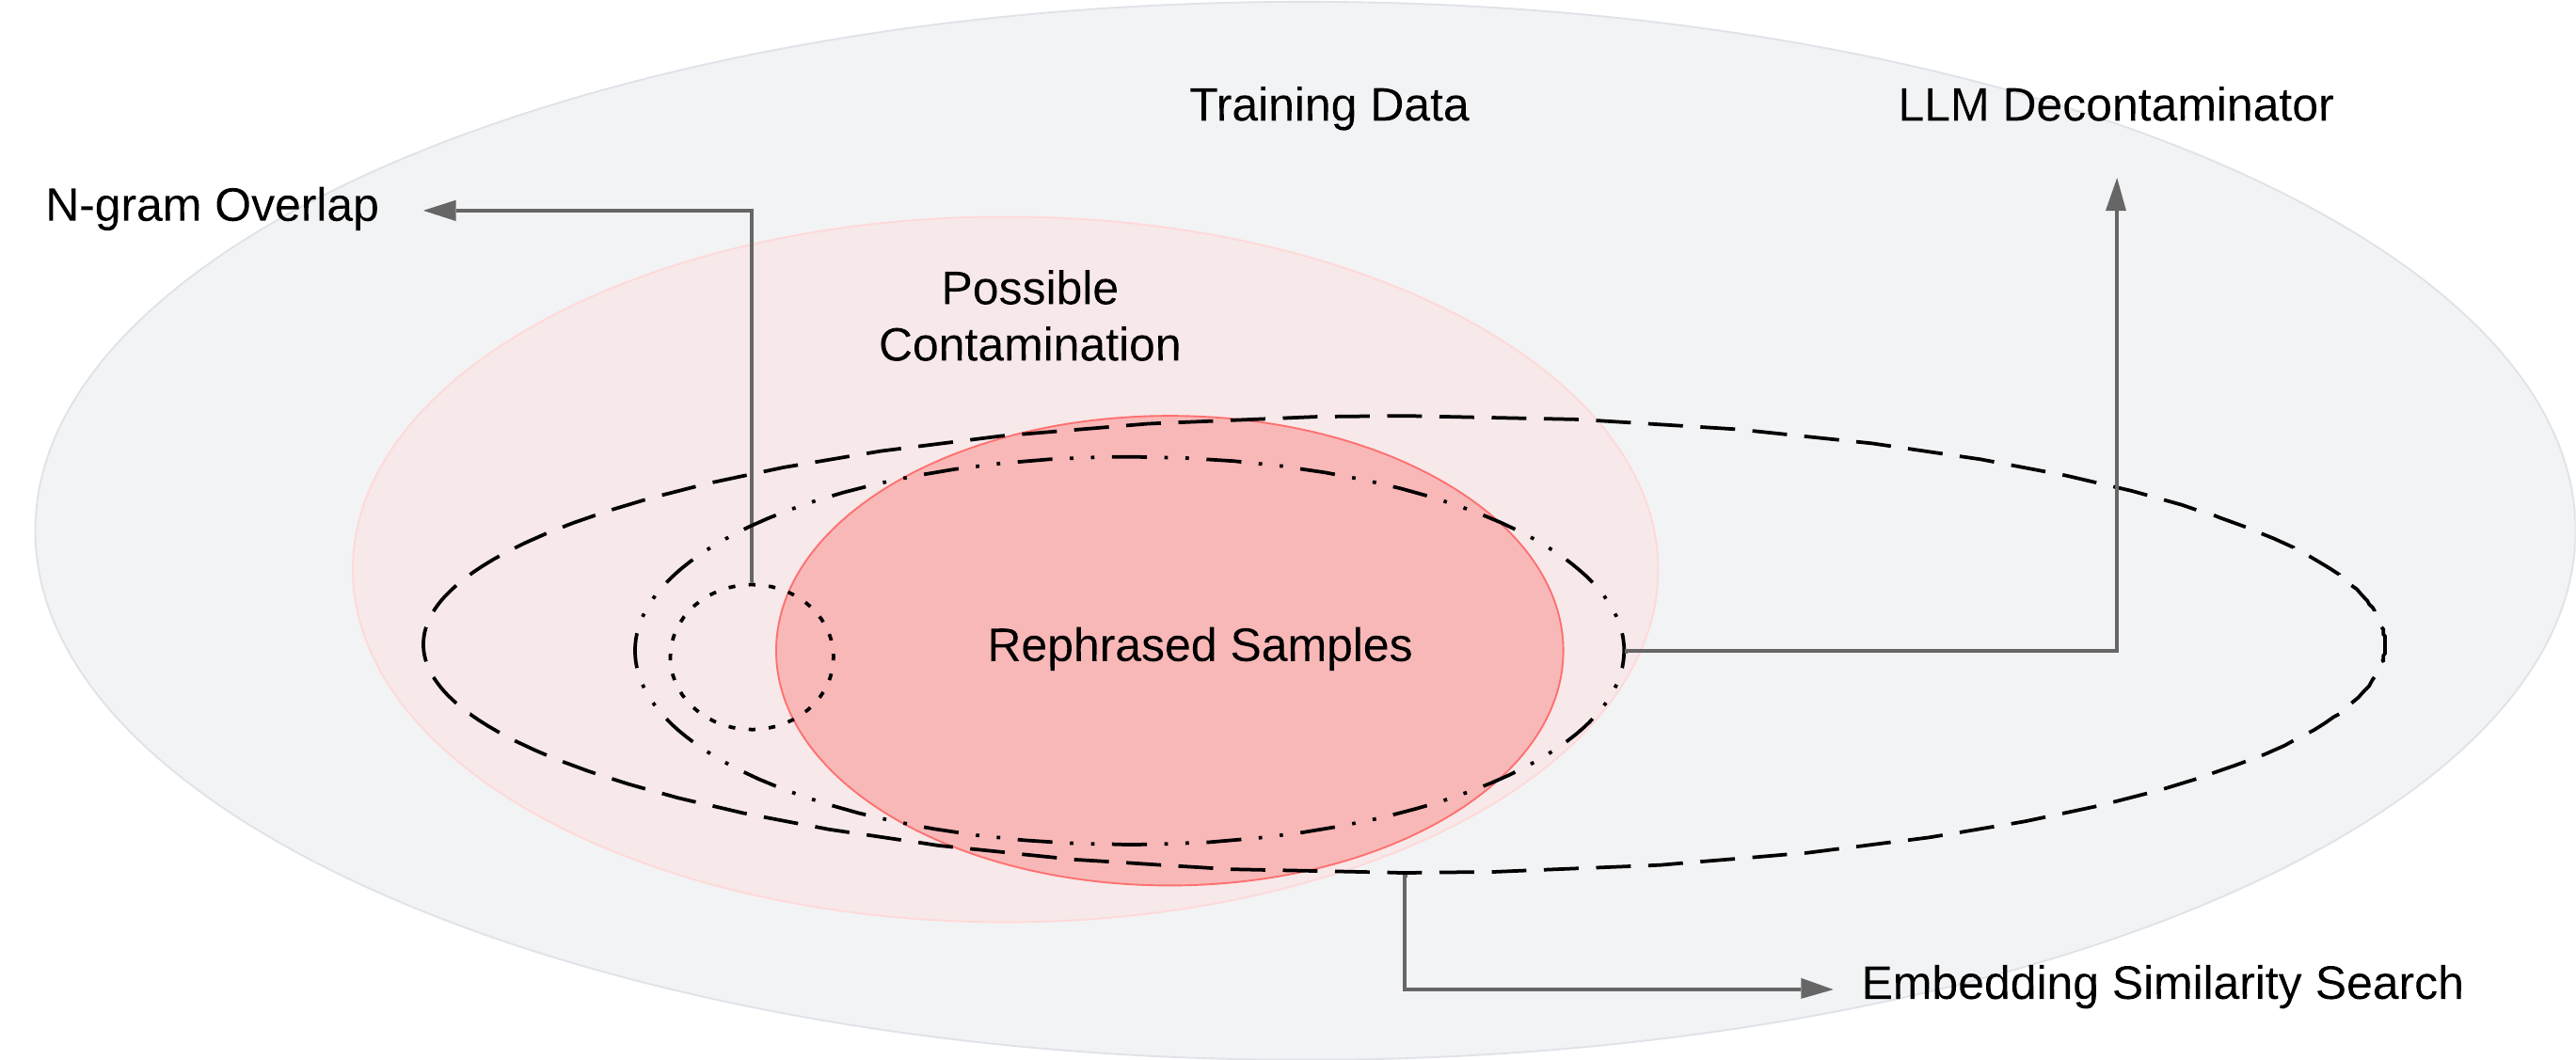
\includegraphics[width=0.9\textwidth]{contamination_venn-v2.png}
\caption{Venn graph depicting training data subsets and contamination detection ranges.
% Solid sections indicate training data and its subsets, while hollow sections highlight areas marked as contaminated by detection methods.
The solid circle represents the training data and its subsets.
The dashed circles enclose areas flagged for potential contamination by detection methods within the dataset.
Notably, the LLM decontaminator showcases higher accuracy.
Embedding similarity search detects broadly but with many false positives. N-gram overlap has a limited ability to spot rephrased samples. The LLM decontaminator refines the results from embedding similarity search using LLMs, providing a precise and efficient contamination assessment.
}
\label{fig:spectrum}
\vspace{-25pt}
\end{figure*}


% \subsection{experiments}

% The rephrase contamination dataset created in section 3.4 was examined using the LLM Decontaminator. The complete f1 score table can be found in the appendix.




% \subsection{real world dataset}

% % We applied the decontamination method on popular real-world datasets and discovered a substantial amount of rephrase contamination. It's highly likely that these contaminations, similar to the experiments in section 3.4, inflate the benchmark evaluation. We will present the number of detected rephrase contaminations as well as some rephrased test cases.

% We used the LLM Decontamination on well-known real-world datasets and discovered significant rephrase contamination. Similar to the tests in section 3.4, it is very likely that these contaminations exaggerate the benchmark evaluation. 


% \textbf{FLAN}~\citep{longpre2023flan} is a sizable knowledge training dataset. We chose to examine a subset called CoT, which accounts for 1.63\% of FLAN, due to its size and variety of data sources. We utilized GPT-4 for detection and set k=1 for the decontamination parameters. The findings show that 76 test cases, or 0.543\% of the MMLU test set, were contaminated.


% \begin{tcolorbox}[title={FLAN CoT Contamination Example}]
% \begin{multicols}{2}

% \textbf{MMLU test} \newline 

% Question: \\
% What type of meat is on a traditional Reuben sandwich?
%     \begin{itemize}
%         \item[A.] turkey
%         \item[B.] bologna
%         \item[C.] corned beef
%         \item[D.] pepperoni
%     \end{itemize}

% Answer: C

% \columnbreak 

% \textbf{FLAN CoT} \newline

% Question: \\
% The Reuben sandwich is an American hot sandwich composed of corned beef, Swiss cheese, sauerkraut, and Russian dressing, grilled between slices of rye bread. Several variants exist.

% What is the meat in a reuben sandwich? Let's have some stream of consciousness first. \\
% % Answer: \\
% % The relevant sentence in the passage is: The Reuben sandwich is an American hot sandwich composed of corned beef, Swiss cheese, sauerkraut, and Russian dressing, grilled between slices of rye bread. So, the answer is corned beef.
% \end{multicols}
% \end{tcolorbox}


% \textbf{CodeAlpaca}~\citep{codealpaca} contains 20K instruction-following data used for fine-tuning the Code Alpaca model. 
% Codealpaca-20K was used to train a number of well-known models, including Tulu~\citep{wang2023far}. 
% We also employed GPT-4 for detection with k=1 as the parameter. The results reveal that there are 21 contaminated test cases on HumanEval, accounting for 12.8\% of HumanEval.


% \begin{tcolorbox}[title={CodeAlpaca Contamination Example}]
% \begin{multicols}{2}

% % HumanEval test code
% \begin{tcolorbox}[title={HumanEval test}, enhanced, colback=white, boxrule=1pt, sharp corners, boxsep=5pt, left=5pt, right=5pt, top=5pt, bottom=5pt]
% \fontsize{8pt}{9.6pt}\selectfont
% \begin{minted}{python}
% def sum_to_n(n: int):
%     """sum_to_n is a function that 
%     sums numbers from 1 to n.
%     >>> sum_to_n(30)
%     465
%     >>> sum_to_n(100)
%     5050
%     >>> sum_to_n(5)
%     15
%     >>> sum_to_n(10)
%     55
%     >>> sum_to_n(1)
%     1
%     """
%     return sum(range(n + 1))
% \end{minted}
% \end{tcolorbox}

% \columnbreak

% % CodeAlpaca code
% \begin{tcolorbox}[title={CodeAlpaca}, enhanced, colback=white, boxrule=1pt, sharp corners, boxsep=5pt, left=5pt, right=5pt, top=5pt, bottom=5pt]
% \fontsize{8pt}{9.6pt}\selectfont
% \begin{minted}{python}
% """
% Create a code that summation 
% of all numbers between 1 to n.
% """

% def sum_all_nums(n):
%     res = 0
    
%     for i in range(1, n+1):
%         res += i
    
%     return res


% print(sum_all_nums(n)) # 15
% \end{minted}
% \end{tcolorbox}

% \end{multicols}
% \end{tcolorbox}




% \textbf{MATH}~\citep{hendrycksmath2021} is one of the most widely used datasets for training mathematical capabilities. It encompasses various branches of mathematics, including algebra, geometry, number theory, and more. It has been utilized in the construction of many math datasets, including MathInstruct~\citep{yue2023mammoth}. Within MATH, we identified 79 instances of self-rephrase contamination, making up 1.58\% of the MATH test set.


% \begin{tcolorbox}[title={MATH Contamination Example}]
% \begin{multicols}{2}

% \textbf{MATH test} \newline 

% How many three-digit positive integers are multiples of 11?

% \columnbreak 

% \textbf{MATH} \newline

% How many positive 3-digit numbers are divisible by 11?

% \end{multicols}
% \end{tcolorbox}

% We examined numerous datasets in addition to those already stated. The appendix contains information on the possible contamination of these datasets as well as examples of contamination.




\section{Experiments}

% In this section, we demonstrate the effectiveness of rephrased samples on MMLU, HumanEval, and GSM-8k, and verify instances of rephrased samples in real-world datasets.
In Section~\ref{sec:rephrase-exp}, we demonstrate that models trained on rephrased samples can achieve dramatically high scores, achieving GPT-4 performance in three widely used benchmarks, MMLU, HumanEval, and GSM-8k.
% These results indicate that rephrased samples are contamination that should be removed from datasets.
This suggests that rephrased samples should be considered as contamination and should be removed from training data.
% \weilin{this suggests rephrased samples should be considered contamination and should be removed from training data.}
In Section~\ref{sec:detect-rephrase}, we evaluate different contamination detection methods based on rephrased samples in MMLU/HumanEval.
In Section \ref{sec:real-world}, we apply our decontaminator to widely-used training sets and discover previously unknown contamination.
% \weilin{In Section~\ref{sec:real-world}, we apply our decontaminator to widely-used training data and discover ...}We also discovered previous unknown contamination in real-world datasets with the LLM decontaminator.

\subsection{Rephrased Samples Contaminate Benchmarks}
\label{sec:rephrase-exp}

\subsubsection{MMLU Knowledge Benchmark}
\label{sec:false_pos}
MMLU~\citep{hendrycks2020mmlu} is one of the benchmarks with the widest range of subjects, covering 57 disciplines from abstract algebra to professional psychology. Rephrasing MMLU requires considering a multitude of scenarios. Given the complexity of MMLU and its multiple-choice format, it is necessary to explain the rephrasing details involved.


\textbf{False positive issue}. The use of n-gram overlap detection in multiple-choice questions can easily result in false positives, especially when different questions share similar option arrangements.
% \weilin{refer reader to the below example here.} 
% Below is a false positive example of a multiple-choice question. 
Example \ref{def:false-positive-example} is a false positive example from n-gram overlap detection. Even though their multi-choice answer patterns match exactly, they are indeed different problems.
% \weilin{Below is a false positive example from n-gram overlap detection. Even though their multi-choice answer patterns match exactly, they are indeed different problems.}
To reduce false positive issues, we introduce a ``question only'' control group in MMLU experiments. 
``Question Only'' refers to rephrasing just the question stem, while ``Full Prompt'' refers to rephrasing both the question stem and the options.
% which only rephrases the stem of multi-choice questions and does not rephrase the answer options.
% \weilin{briefly explain what's ``quesiton only''}

% Using n-gram overlap detection in multiple-choice questions can easily lead to false positives. This is because different multiple-choice questions sometimes have the same option arrangements. Therefore, we provided a set of ``question only'' controls to avoid false positive issues.

% \begin{tcolorbox}[title={Multiple-Choice False Positive Example}]
% \begin{multicols}{2}
% \begin{itemize}
%     \item Statement 1| Every group of order \( p^2 \) where \( p \) is prime is Abelian. \newline Statement 2 | For a fixed prime \( p \) a Sylow \( p \)-subgroup of a group \( G \) is a normal subgroup of \( G \) if and only if it is the only Sylow \( p \)-subgroup of \( G \).
%     \begin{itemize}
%         \item[\textcolor{red}{A.}] \textcolor{red}{True, True}
%         \item[\textcolor{red}{B.}] \textcolor{red}{False, False}
%         \item[\textcolor{red}{C.}] \textcolor{red}{True, False}
%         \item[\textcolor{red}{D.}] \textcolor{red}{False, True}
%     \end{itemize}

%     \columnbreak
    
%     \item Statement 1 | Every group of order 42 has a normal subgroup of order 7. \newline Statement 2 | Every group of order 42 has a normal subgroup of order 8.
%     \begin{itemize}
%         \item[\textcolor{red}{A.}] \textcolor{red}{True, True}
%         \item[\textcolor{red}{B.}] \textcolor{red}{False, False}
%         \item[\textcolor{red}{C.}] \textcolor{red}{True, False}
%         \item[\textcolor{red}{D.}] \textcolor{red}{False, True}
%     \end{itemize}
% \end{itemize}
% \end{multicols}
% \end{tcolorbox}

\begin{example}[Multi-Choice False Positive]\label{def:false-positive-example}
\begin{itemize}
    \item Statement 1| Every group of order \( p^2 \) where \( p \) is prime is Abelian. \\
    Statement 2 | For a fixed prime \( p \) a Sylow \( p \)-subgroup of a group \( G \) is a normal subgroup of \( G \) if and only if it is the only Sylow \( p \)-subgroup of \( G \).
    \begin{itemize}[noitemsep]
        \item[\textcolor{red}{A.}] \textcolor{red}{True, True}
        \item[\textcolor{red}{B.}] \textcolor{red}{False, False}
        \item[\textcolor{red}{C.}] \textcolor{red}{True, False}
        \item[\textcolor{red}{D.}] \textcolor{red}{False, True}
    \end{itemize}
    
    %\vspace{0.5cm} % Adds some space between the two contents

    \item Statement 1 | Every group of order 42 has a normal subgroup of order 7. \\
    Statement 2 | Every group of order 42 has a normal subgroup of order 8.
    \begin{itemize}[noitemsep]
        \item[\textcolor{red}{A.}] \textcolor{red}{True, True}
        \item[\textcolor{red}{B.}] \textcolor{red}{False, False}
        \item[\textcolor{red}{C.}] \textcolor{red}{True, False}
        \item[\textcolor{red}{D.}] \textcolor{red}{False, True}
    \end{itemize}
\end{itemize}

\end{example}

\textbf{Other details}. 
Large numbers often induce character overlap. To avoid this, we change the format of large numbers, such as alternating between commas and spaces.
% In arithmetic tests with large numbers, we alternate between commas and spaces to avoid character overlap. \weilin{this sentence is hard to understand} 
Proprietary terms in various domains can also trigger overlap issues. To circumvent this, we rotate between abbreviations and full terms and adjust capitalization, particularly when choices involve names or chemical formulas.

% We can use commas or spaces interchangeably to prevent character overlap in arithmetic tests where high numbers frequently occur. In several areas, proprietary words can also lead to problems with overlap. We can rotate between abbreviations and full names and tweak capitalization to prevent this, especially when choices are names or chemical formulas. This keeps the model clear and lowers the danger of detection.

\textbf{Benchmark results}. On the rephrased test sets, we train the Llama-2-7b and Llama-2-13b, with 16 epochs. 
% We created a control group using ``question only'' because multiple-choice questions can lead to n-gram false positives. 
% Due to the issue of n-gram overlap false positives in multiple-choice questions, we introduce a ``question only'' control group. 
As shown in Table \ref{table:mmlu_basic_stats}, 
Llama-2 7B and 13B trained on rephrased samples can achieve dramatically high scores on MMLU, from 45.3 to 88.5.
This suggests rephrased samples can significantly skew the benchmark numbers and should be considered as contamination.
The original model is tested on 5-shot, and the model trained on rephrased data is tested on 0-shot.
% \weilin{consider explictly say number. e.g., from 45.3 to 88.5}
% \todo{writing improve}
% Although clean training sets can not entirely eliminate n-gram overlap, rephrased full prompts can, rendering the ``question only'' approach a fairer comparison.
% Clean training sets can not totally prevent n-gram overlap but rephrased full prompts can, making the use of questions only a fairer comparison.


\begin{table}[t]
\centering
\caption{Accuracy on MMLU. ``Rephrased Chinese'' refers to translating the questions into Chinese.}
\label{table:mmlu_basic_stats}
\footnotesize
\begin{tabular}{lccc}
\toprule
Model & Original & \multicolumn{2}{c}{Rephrased English} \\
\cmidrule(lr){3-4}
& & Question Only & Full Prompt \\
\midrule
Llama 2 7B   & 45.3 & 88.5 & 82.0 \\
Llama 2 13B  & 54.8 & 89.9 & 85.9 \\
\midrule
Model & Test Set & \multicolumn{2}{c}{Rephrased Chinese} \\
\cmidrule(lr){3-4}
& & Question Only & Full Prompt \\
\midrule
Llama 2 7B   & 100 & 91.1 & 74.3 \\
Llama 2 13B  & 100 & 93.7 & 80.9 \\
\bottomrule
\end{tabular}
\vspace{-10pt}
\end{table}

\subsubsection{HumanEval Coding Benchmark}
% \todo{need review @lianmin}

HumanEval~\citep{chen2021humaneval} is a benchmark provided by OpenAI to evaluate the coding capabilities of large language models. It provides the model with an incomplete piece of code and asks the model to complete it. 
% This benchmark closely reaches real-world coding scenarios and can effectively evaluate the model's coding capabilities.

% \todo{tone: won't affect semantic}
\textbf{Dead code injection}. In real-world coding datasets, there are some unreachable instructions. These dead codes seldom affect the semantics, and they help rephrased samples to escape decontamination.
% To evade n-gram overlap detection, dead code injection can effectively avoid repetition. 
Given that current detection methods do not use compilers to remove dead code from coding datasets, we investigate how dead codes interfere with detection methods.


\textbf{Benchmark results}. We rephrase the HumanEval test set in Python and translate it into five programming languages: C, JavaScript, Rust, Go, and Java. We train CodeLlama 7B and 13B on these codes respectively. Then, we construct a multi-programming-language dataset comprising the five programming languages and train on it. Table \ref{table:humaneval_basic_stats} shows CodeLlama's performance on rephrased Python, rephrased C, and the multi-programming-language dataset.
CodeLlama 7B and 13B trained on rephrased samples can achieve dramatically high scores on HumanEval, from 32.9 to 67.7 and 36.0 to 81.1, respectively.
In contrast, GPT-4 can only achieve 67.0 on HumanEval.
% \weilin{mention gpt-4 performance?}

% \begin{table}[h]
% \centering
% \caption{Pass@1 on HumanEval.}
% \label{table:basic_stats}
% \footnotesize
% %\resizebox{1\textwidth}{!}{% <------ Don't forget this %
% \begin{tabular}{cccccc}
% \toprule
% \multirow{2}{*}{Model} & \multirow{2}{*}{Original} & Fine-tune on & Fine-tune on & Fine-tune on & Fine-tune on \\
% &  &  test set & rephrased Python & rephrased C & Multi-languages \\
% \midrule
% CodeLlama 7B   & 32.9   &  100   & 67.7 & 45.7 &  59.8 \\
% CodeLlama 13B  & 36.0   &  100   & 81.1 & 48.2 &  67.1 \\
% \bottomrule
% \end{tabular}
% %}
% \end{table}

\begin{table}[t]
\centering
\caption{Pass@1 on HumanEval.}
\label{table:humaneval_basic_stats}
\footnotesize

\begin{tabular}{lccc}
\toprule
Model & Original & & Fine-tune on test set \\
\midrule
CodeLlama 7B   & 32.9 & & 100 \\
CodeLlama 13B  & 36.0 & & 100 \\
\midrule
Model & \multicolumn{3}{c}{Fine-tune on rephrased} \\
\cmidrule(lr){2-4}
& Python & C & Multi-languages \\
\midrule
CodeLlama 7B   & 67.7 & 45.7 & 59.8 \\
CodeLlama 13B  & 81.1 & 48.2 & 67.1 \\
\bottomrule
\end{tabular}
\vspace{-10pt}
\end{table}


% \begin{table}[h]
% \centering
% \caption{Accuracy on MMLU.}
% \label{table:basic_stats}
% \footnotesize
% \begin{tabularx}{\linewidth}{lcccccc}
% \toprule
% \multirow{3}{*}{Model} & \multirow{3}{*}{Original} & \multirow{3}{*}{ test set} & \multicolumn{2}{c}{ rephrased English} & \multicolumn{2}{c}{ rephrased Chinese} \\
% \cmidrule(lr){4-5} \cmidrule(lr){6-7}
% & & & question only & full prompt & question only & full prompt \\
% \midrule
% Llama 2 7B   &   45.3    &   100    &  88.5   &  82.0 &  91.1 & 74.3 \\
% Llama 2 13B  &   54.8    &   100    &  89.9   &  85.9 &  93.7 & 80.9 \\
% \bottomrule
% \end{tabularx}
% \end{table}




\subsubsection{GSM-8K Math Benchmark}

GSM-8K~\citep{cobbe2021gsm8k} is a commonly used benchmark for testing the mathematical capabilities of LLMs. 
% It contains many question-answer pairs, where the LLM generates the solution based on the question. 
% The solution ends with four `\#' characters, after which the answer should be provided. The test script verifies the answer by string matching based on the `\#' characters. 
% \weilin{why are we mentioning these details?}
% We use the rephrased test set to fine-tune Llama-2 7b and 13b, and they achieve dramatically high scores on GSM-8K.

\textbf{Benchmark results}. Table \ref{table:gsm8k_basic_stats} shows that Llama-2 7b and 13b trained on rephrased samples achieve dramatically high scores on GSM-8K, from 28.7 to 95.3.
% The models trained on rephrased samples are tested with 0-shot.
The original model is tested on 5-shot, and the model trained on rephrased data is tested on 0-shot.


\begin{table}[t]
\centering
\caption{Accuracy on GSM-8K.}
\label{table:gsm8k_basic_stats}
\footnotesize
\begin{tabular}{cccc}
\toprule
\multirow{2}{*}{Model} & \multirow{2}{*}{Original} & Fine-tune on & Fine-tune on \\
&  &  test set & rephrased English \\
\midrule
Llama 2 7B   &   14.6    &    100    &   86.7 \\
Llama 2 13B  &   28.7    &    100    &   95.3 \\
\bottomrule
\end{tabular}
\vspace{-10pt}
\end{table}

We will explore the detection problems in Section~\ref{sec:one-time-exam} with GSM-8k as they relate to the ``number substituted only case''.
% \weilin{I think we can remove this.}


% We tested three subjects, including abstract algebra, sociology, and US history.
% We created 200 prompt pairs utilizing the original test set and the rephrased test set in order to evaluate the detection effectiveness of various approaches against the rephrased samples. 100 random pairs and 100 rephrased pairs are included. We can determine whether the rephrased samples avoids detection by calculating the F1 score on these pairs; lower values signify more effective evasion.
% \weilin{I'd still suggest a subsection here to make a clear transition from the above. or we probably should just not combine the two experiments in the same subsection.}

\subsection{Evaluating Contamination Detection Methods}
\label{sec:detect-rephrase}

%In this section, we show that existing detection methods can fail to detect rephrased samples.
%while the LLM decontaminator succeeds in detecting them.
\subsubsection{MMLU}
We construct a decontamination benchmark based on three subjects: abstract algebra, sociology, and US history in MMLU.
To compare the accuracy of detection methods against rephrased samples, we construct 200 prompt pairs using both the original and rephrased test sets. These comprised 100 random pairs and 100 rephrased pairs. The f1 score on these pairs provides insight into the detection methods' ability to detect contamination, with higher values indicating more precise detection.

\begin{figure*}[h]
\centering
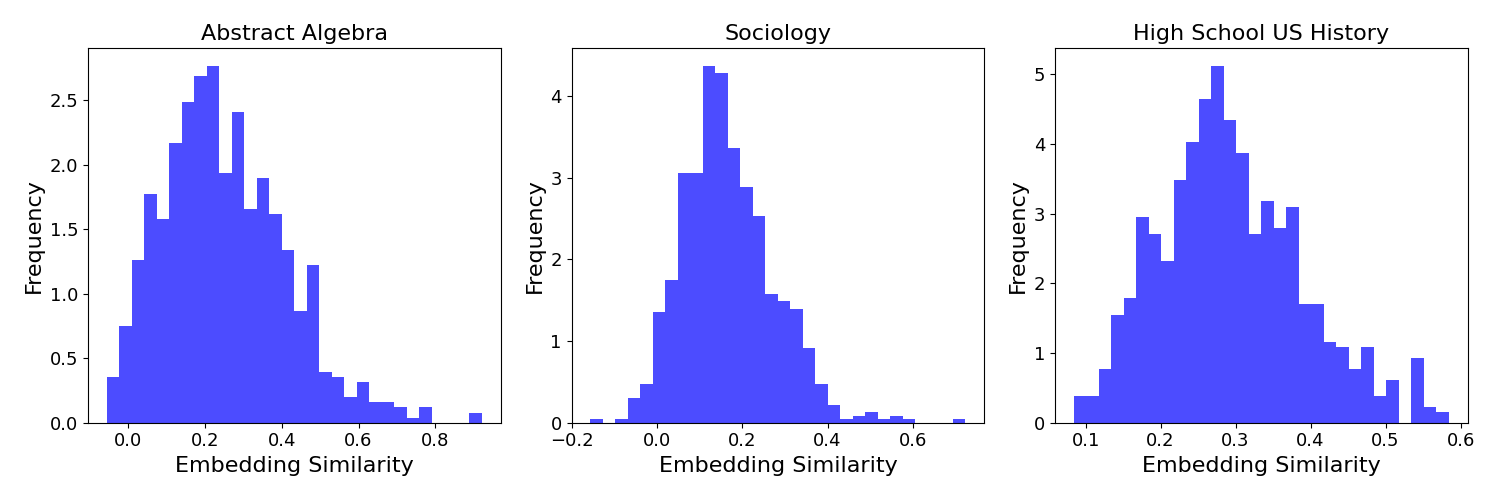
\includegraphics[width=0.9\textwidth]{sim_inside_mmlu_v3.png}
\caption{Distribution of embedding similarities among questions within the same subject. Note that it is difficult to set a unified threshold to decontaminate due to the vast differences between subjects.  
For example, if we adjust the threshold to 0.8, ``Abstract Algebra'' may be properly spotted, but rephrased samples in ``Sociology'' become difficult to identify. If the threshold is set to 0.4, ``Abstract Algebra'' will produce a large number of false positives.
}
\label{fig:embedding_similarity}
\vspace{-20pt}
\end{figure*}


% We employed random detection as our baseline, with scores significantly surpassing this indicating a detection method's effectiveness. For the n-gram overlap detection, we opted for a 10-gram. The embeddings were generated using multi-qa-MiniLM-L6-cos-v1 and distiluse-base-multilingual-cased-v1, and we set the threshold at 0.5.

We use random detection as our baseline, where scores significantly above random detection indicate the effectiveness of a detection method. For n-gram overlap, we choose a 10-gram approach. The embeddings are generated by multi-qa-MiniLM-L6-cos-v1 and distiluse-base-multilingual-cased-v1~\citep{reimers-2019-sentence-bert}, with a threshold of 0.5. 
% \weilin{add citation}
% The models trained on rephrased samples are tested with 0-shot.


% \begin{table}[h]
% \centering
% \caption{F1 scores of different detection methods on MMLU.}
% \label{table:f1_scores}
% \footnotesize
% \begin{tabular}{l|ccc|ccc|ccc}
% \toprule
% & \multicolumn{3}{c|}{Test Set} & \multicolumn{3}{c|}{Rephrased English} & \multicolumn{3}{c}{Rephrased Chinese} \\
% \midrule
% Subjects & Alg. & Soc. & Hist. & Alg. & Soc. & Hist. & Alg. & Soc. & Hist. \\
% \midrule
% Random & 0.500 & 0.500 & 0.500 & 0.500 & 0.500 & 0.500 & 0.500 & 0.500 & 0.500 \\
% 10-gram & 0.926 & 1 & 0.816 & 0 & 0 & 0 & 0 & 0 & 0 \\
% Embed (Multi-QA BERT) & 0.990 & 0.995 & 0.980 & 0.985 & 0.985 & 0.805 & 0.179 & 0.020 & 0 \\
% Embed (Multilingual BERT) & 0.939 & 1 & 0.990 & 0.934 & 0.985 & 0.111 & 0.939 & 1 & 0.985 \\
% LLM Decontaminator & 1 & 1 & 1 & 0.960 & 0.940 & 0.970 & 0.990 & 0.950 & 0.980 \\
% \bottomrule
% \end{tabular}
% \end{table}

% \begin{table*}[h]
% \centering
% \caption{F1 scores of different detection methods on MMLU. \textbf{REORGANIZE}}
% \label{table:f1_scores}
% \footnotesize
% \begin{tabularx}{\textwidth}{l|XXX|XXX|XXX}
% \toprule
% & \multicolumn{3}{c|}{Test Set} & \multicolumn{3}{c|}{Rephrased English} & \multicolumn{3}{c}{Rephrased Chinese} \\
% \midrule
% Subjects & Alg. & Soc. & Hist. & Alg. & Soc. & Hist. & Alg. & Soc. & Hist. \\
% \midrule
% Random & 0.500 & 0.500 & 0.500 & 0.500 & 0.500 & 0.500 & 0.500 & 0.500 & 0.500 \\
% 10-gram & 0.926 & 1 & 0.816 & 0 & 0 & 0 & 0 & 0 & 0 \\
% Emb (Multi-QA BERT) & 0.990 & 0.995 & 0.980 & 0.985 & 0.985 & 0.805 & 0.179 & 0.020 & 0 \\
% Emb (Multilingual BERT) & 0.939 & 1 & 0.990 & 0.934 & 0.985 & 0.111 & 0.939 & 1 & 0.985 \\
% LLM Decontaminator & 1 & 1 & 1 & 0.960 & 0.940 & 0.970 & 0.990 & 0.950 & 0.980 \\
% \bottomrule
% \end{tabularx}
% \end{table*}


% \begin{table*}[h]
% \centering
% \caption{F1 scores of different detection methods on MMLU.}
% \label{table:f1_scores}
% \footnotesize
% \begin{tabularx}{\textwidth}{l|XXX|XXX|XXX}
% \toprule
% & \multicolumn{3}{c|}{Algebra} & \multicolumn{3}{c|}{Sociology} & \multicolumn{3}{c}{US History} \\
% \midrule
% Subjects & Test Set & Rephrased English & Rephrased Chinese & Test Set & Rephrased English & Rephrased Chinese & Test Set & Rephrased English & Rephrased Chinese \\
% \midrule
% Random & 0.500 & 0.500 & 0.500 & 0.500 & 0.500 & 0.500 & 0.500 & 0.500 & 0.500 \\
% 10-gram & 0.926 & 0 & 0 & 1 & 0 & 0 & 0.816 & 0 & 0 \\
% Emb (Multi-QA BERT) & 0.990 & 0.985 & 0.179 & 0.995 & 0.985 & 0.020 & 0.980 & 0.805 & 0 \\
% Emb (Multilingual BERT) & 0.939 & 0.934 & 0.939 & 1 & 0.985 & 1 & 0.990 & 0.111 & 0.985 \\
% LLM Decontaminator & 1 & 0.960 & 0.990 & 1 & 0.940 & 0.950 & 1 & 0.970 & 0.980 \\
% \bottomrule
% \end{tabularx}
% \vspace{-10pt}
% \end{table*}

\begin{table*}[h]
\centering
\caption{F1 scores of different detection methods on MMLU. The bold numbers indicate that the detection is reliable.}
\label{table:f1_scores}
\footnotesize
\begin{tabularx}{\textwidth}{l|XXX|XXX|XXX}
\toprule
& \multicolumn{3}{c|}{Algebra} & \multicolumn{3}{c|}{Sociology} & \multicolumn{3}{c}{US History} \\
\midrule
Subjects & Test Set & Rephrased English & Rephrased Chinese & Test Set & Rephrased English & Rephrased Chinese & Test Set & Rephrased English & Rephrased Chinese \\
\midrule
Random & 0.500 & 0.500 & 0.500 & 0.500 & 0.500 & 0.500 & 0.500 & 0.500 & 0.500 \\
10-gram & \textbf{0.926} & 0 & 0 & \textbf{1} & 0 & 0 & 0.816 & 0 & 0 \\
Emb (Multi-QA BERT) & \textbf{0.990} & \textbf{0.985} & 0.179 & \textbf{0.995} & \textbf{0.985} & 0.020 & \textbf{0.980} & 0.805 & 0 \\
Emb (Multilingual BERT) & \textbf{0.939} & \textbf{0.934} & \textbf{0.939} & \textbf{1} & \textbf{0.985} & \textbf{1} & \textbf{0.990} & 0.111 & \textbf{0.985} \\
LLM Decontaminator & \textbf{1} & \textbf{0.960} & \textbf{0.990} & \textbf{1} & \textbf{0.940} & \textbf{0.950} & \textbf{1} & \textbf{0.970} & \textbf{0.980} \\
\bottomrule
\end{tabularx}
\vspace{-10pt}
\end{table*}




% \begin{table}[h]
% \centering
% \caption{F1 scores for different detect methods under rephrase attack.}
% \label{table:f1_scores}
% \footnotesize
% \begin{tabular}{l|ccc|ccc|ccc}
% \toprule
% & \multicolumn{3}{c|}{Test Set} & \multicolumn{3}{c|}{Rephrased English} & \multicolumn{3}{c}{Rephrased Chinese} \\
% \midrule
% Subjects & Alg. & Soc. & Hist. & Alg. & Soc. & Hist. & Alg. & Soc. & Hist. \\
% \midrule
% Rand & 0.5 & 0.5 & 0.5 & 0.5 & 0.5 & 0.5 & 0.5 & 0.5 & 0.5 \\
% 10-gram & 0.926 & 1 & 0.816 & 0 & 0 & 0 & 0 & 0 & 0 \\
% Multi-QA Bert & 0.99 & 0.995 & 0.98 & 0.985 & 0.985 & 0.805 & 0.179 & 0.02 & 0 \\
% Multilingual Bert & 0.939 & 1 & 0.99 & 0.934 & 0.985 & 0.111 & 0.939 & 1 & 0.985 \\
% \bottomrule
% \end{tabular}
% \end{table}

% From the results, aside from the LLM decontaminator, we found that all detection methods introduced some false positives. Both the rephrased samples and translated samples successfully evaded n-gram overlap detection. When using multi-qa bert, the embedding similarity search couldn't detect the translated samples at all. When we employed multilingual bert, the embedding similarity search failed to detect contamination in the US History subject. LLM decontaminator detected contamination with very high stability and accuracy.

As shown in Table \ref{table:f1_scores}, except for the LLM decontaminator, all other detection methods introduce some false positives. Both rephrased and translated samples are undetected by the n-gram overlap. With multi-qa BERT, the embedding similarity search proves completely ineffective against translated samples. When using multilingual BERT, this method struggles with the US History subject. 
% Notably, the LLM decontaminator showcases superior performance, identifying rephrased samples with almost perfect precision and recall.
The LLM decontaminator's reliability and precision are evidenced by the highest minimum and average f1 scores.
% Following the approach we took with mmlu, we constructed 200 prompt pairs on HumanEval and calculated the F1 score using n-gram, embedding similarity search, and LLM decontaminator. For n-gram detection, we used a 10-gram overlap and a 50-character overlap. To generate embeddings for the similarity search, we utilized CodeLlama and multi-qa-MiniLM-L6-cos-v1, with threshold adjustments set to 0.9 and 0.6, respectively.

% We created 200 prompt pairs on HumanEval using the same methodology we used with MMLU, and we used n-gram overlap, embedding similarity search, and LLM decontaminator to determine the F1 score. We employed a 10-gram overlap and a 50-character overlap for n-gram overlap detection. We used CodeLlama and multi-qa-MiniLM-L6-cos-v1 to generate embeddings for the similarity search, with threshold adjustments set to 0.9 and 0.6, respectively.

% \todo{change}
\subsubsection{HumanEval}
Now we show that existing detection methods fail to detect rephrased samples of HumanEval, while the LLM decontaminator succeeds in detecting them.
For HumanEval, we construct 200 prompt pairs following the method previously outlined for MMLU. For n-gram overlap detection, we use both 10-gram and 50-character overlap. Embeddings are generated by CodeLlama and multi-qa-MiniLM-L6-cos-v1, with respective threshold adjustments at 0.9 and 0.6. We evaluate the F1 score using n-gram overlap, embedding similarity search, and LLM decontaminator.


% \begin{table}[h]
% \centering
% \caption{F1 scores of different detection methods on HumanEval.}
% \label{table:new_f1_scores}
% \footnotesize
% \begin{tabular}{l|c|c|c|c}
% \toprule
% & Test Set & Rephrased Python & Rephrased C & Rephrased JavaScript \\
% \midrule
% Random & 0.500 & 0.500 & 0.500 & 0.500 \\
% 10-gram & 1 & 0 & 0 & 0 \\
% Embed (CodeLlama) & 0.966 & 0.903 & 0.438 & 0.503 \\
% Embed (Multi-QA BERT) & 0.985 & 0.938 & 0.774 & 0.788 \\
% LLM Decontaminator & 1 & 0.995 & 0.974 & 0.980 \\
% \bottomrule
% \end{tabular}
% \end{table}

\begin{table}[h]
\centering
\caption{F1 scores of detection methods on HumanEval}
\label{table:new_f1_scores}
\footnotesize
\begin{tabular}{l|c|c|c|c}
\toprule
& \multirow{2}{*}{Test } & \multicolumn{3}{c}{Rephrased} \\
\cmidrule(lr){3-5}
& Set & Python & C & JS \\
\midrule
Random & 0.500 & 0.500 & 0.500 & 0.500 \\
10-gram & 1 & 0 & 0 & 0 \\
Emb (CodeLlama) & \textbf{0.966} & 0.903 & 0.438 & 0.503 \\
Emb (Multi-QA BERT) & \textbf{0.985} & 0.938 & 0.774 & 0.788 \\
LLM Decontaminator & \textbf{1} & \textbf{0.995} & \textbf{0.974} & \textbf{0.980} \\
\bottomrule
\end{tabular}
\vspace{-20pt}
\end{table}




% \begin{table}[h]
% \centering
% \caption{HumanEval F1 Score for Different Detect Methods under Rephrase Attack.}
% \label{table:new_f1_scores}
% \footnotesize
% \begin{tabular}{l|c|c|c|c}
% \toprule
% & Test Set & Rephrased Python & Rephrased C & Rephrased JavaScript \\
% \midrule
% Rand & 0.5 & 0.5 & 0.5 & 0.5 \\
% 10-gram & 1 & 0 & 0 & 0 \\
% CodeLlama & 0.966 & 0.903 & 0.438 & 0.503 \\
% Multi-QA Bert & 0.985 & 0.938 & 0.774 & 0.788 \\
% \bottomrule
% \end{tabular}
% \end{table}


% Based on the F1 scores, we conclude that embedding similarity search is quite effective for detection when used inside the same programming language, but the effect is less noticeable after translation. Only LLM decontaminator can effectively detect coding dataset contamination. The degree of resemblance across programming languages may explain why rephrased C is tougher to spot than rephrased JavaScript. JavaScript and Python are both interpreted languages that provide dynamic typing and some functional programming constructs, so from a syntactical standpoint, JavaScript may be closer to Python.

According to Table \ref{table:new_f1_scores}, we conclude that the embedding similarity search proves effective for detection within the same programming language, but the effect is less noticeable after translation.
Among the methods examined, only the LLM decontaminator reliably detects rephrased samples in coding datasets.
The similarity between programming languages may explain why rephrased C is tougher to spot than rephrased JavaScript. JavaScript and Python are both interpreted languages that provide dynamic typing and some functional programming constructs, so from a syntactical standpoint, JavaScript may be closer to Python.



\subsection{Contamination in Real World Datasets}
\label{sec:real-world}

% We applied the decontamination method on popular real-world datasets and discovered a substantial amount of rephrase contamination. It's highly likely that these contaminations, similar to the experiments in section 3.4, inflate the benchmark evaluation. We will present the number of detected rephrase contaminations as well as some rephrased test cases.

To demonstrate the effectiveness LLM decontaminator, we apply it to widely used real-world datasets and identify a substantial amount of rephrased samples. 
Table \ref{table:dataset_summary} displays the contamination percentage of different benchmarks in each training dataset.
% Based on the results of prior experiments, it is likely that these rephrased samples exaggerate models' benchmark results. 



% \begin{table}[h]
% \centering
% \caption{Rephrased Samples in real-world datasets}
% \label{table:dataset_summary}
% \begin{tabular}{l|l|r|r|r}
% \toprule
% \multirow{2}{*}{Training Set} & \multirow{2}{*}{Benchmark} & Test Set  & Rephrased  & \multirow{2}{*}{Percentage (\%)} \\
% & & Size & Samples & \\
% \midrule
% CodeAlpaca & HumanEval & 164 & 21 & 12.8 \\
% Evol-Instruct-Code & HumanEval & 164 & 13 & 7.93 \\
% CodeExercise-Python & HumanEval & 164 & 26 & 15.9 \\
% rossetacode & HumanEval & 164 & 4 & 2.44 \\
% MATH Train & MATH Test & 5000 & 79 & 1.58 \\
% MATHInstruct & MATH Test & 5000 & 769 & 15.4 \\
% FLAN CoT & MMLU & 14042 & 76 & 0.541 \\
% WizardLM-Evol-Instruct & MMLU & 14042 & 75 & 0.534 \\
% RedPajama-Data-1T (16G subset) & HumanEval & 164 & 14 & 8.53 \\
% The Stack (4G subset) & HumanEval & 164 & 31 & 18.9 \\
% StarCoder (2.4G subset) & HumanEval & 164 & 26 & 15.9 \\
% \bottomrule
% \end{tabular}
% \end{table}

% \begin{table*}[h]
% \centering
% \caption{Rephrased Samples in real-world datasets}
% \label{table:dataset_summary}
% \begin{tabular}{l|l|r|r|r}
% \toprule
% \multirow{2}{*}{Training Set} & \multirow{2}{*}{Benchmark} & Test Set  & Rephrased  & \multirow{2}{*}{Percentage (\%)} \\
% & & Size & Samples & \\
% \midrule
% CodeAlpaca & HumanEval & 164 & 21 & 12.8 \\
% Evol-Instruct-Code & HumanEval & 164 & 13 & 7.93 \\
% CodeExercise-Python & HumanEval & 164 & 26 & 15.9 \\
% rossetacode & HumanEval & 164 & 4 & 2.44 \\
% MATH Train & MATH Test & 5000 & 79 & 1.58 \\
% MATHInstruct & MATH Test & 5000 & 769 & 15.4 \\
% FLAN CoT & MMLU & 14042 & 76 & 0.541 \\
% WizardLM-Evol-Instruct & MMLU & 14042 & 75 & 0.534 \\
% RedPajama-Data-1T (16G subset) & HumanEval & 164 & 14 & 8.53 \\
% The Stack (4G subset) & HumanEval & 164 & 31 & 18.9 \\
% StarCoder-Data (2.4G subset) & HumanEval & 164 & 26 & 15.9 \\
% \bottomrule
% \end{tabular}
% \end{table*}

% \begin{table*}[h]
% \centering
% \caption{The Percentage of Rephrased Sample Contamination in Real-world Datasets.}
% \label{table:dataset_summary}
% \begin{tabular}{l|l|r|r|r|r}
% \toprule
% \multirow{2}{*}{Training Set} & \multirow{2}{*}{Benchmark} & \multicolumn{2}{c|}{Size} & Rephrased  & \multirow{2}{*}{Percentage (\%)} \\
% & & Train Set & Test Set & Samples & \\
% \midrule
% CodeAlpaca & HumanEval & 20k & 164 & 21 & 12.8 \\
% RedPajama-Data-1T (16G subset) & HumanEval & 1625k & 164 & 14 & 8.53 \\
% The Stack (4G subset) & HumanEval & 500k & 164 & 31 & 18.9 \\
% StarCoder-Data (2.4G subset) & HumanEval & 500k & 164 & 26 & 15.9 \\
% Evol-Instruct-Code & HumanEval & 78.3k & 164 & 13 & 7.93 \\
% CodeExercise-Python & HumanEval & 27k & 164 & 26 & 15.9 \\
% rossetacode & HumanEval & 4.26k & 164 & 4 & 2.44 \\
% MATH Train & MATH Test & 7.5k & 5000 & 79 & 1.58 \\
% MATHInstruct & MATH Test & 262k & 5000 & 769 & 15.4 \\
% FLAN CoT & MMLU & 184k & 14042 & 76 & 0.541 \\
% WizardLM-Evol-Instruct & MMLU & 143k & 14042 & 75 & 0.534 \\

% \bottomrule
% \end{tabular}
% \end{table*}

\begin{table*}[h]
\centering
\caption{The Percentage of \# Rephrased Sample Contamination in Real-world Datasets.}
\label{table:dataset_summary}
\begin{tabular}{l|l|r|r|r|r}
\toprule
\multirow{2}{*}{Training Set} & \multirow{2}{*}{Benchmark} & \multicolumn{2}{c|}{Size} & Rephrased  & \multirow{2}{*}{Percentage (\%)} \\
& & Train Set & Test Set & Samples & \\
\midrule
The Stack (4G subset) & HumanEval & 500k & 164 & 31 & 18.9 \\
StarCoder-Data (2.4G subset) & HumanEval & 500k & 164 & 26 & 15.9 \\
CodeExercise-Python & HumanEval & 27k & 164 & 26 & 15.9 \\
CodeAlpaca & HumanEval & 20k & 164 & 21 & 12.8 \\
RedPajama-Data-1T (16G subset) & HumanEval & 1625k & 164 & 14 & 8.5 \\
Evol-Instruct-Code & HumanEval & 78.3k & 164 & 13 & 7.9 \\
rossetacode & HumanEval & 4.26k & 164 & 4 & 2.4 \\
MATHInstruct & MATH Test & 262k & 5000 & 769 & 15.4 \\
MATH Train & MATH Test & 7.5k & 5000 & 79 & 1.6 \\
FLAN CoT & MMLU & 184k & 14042 & 76 & 0.5 \\
WizardLM-Evol-Instruct & MMLU & 143k & 14042 & 75 & 0.5 \\
\bottomrule
\end{tabular}
\end{table*}




% \begin{table}[h]
% \centering
% \caption{Rephrased Samples in real-world datasets}
% \label{table:dataset_summary}
% \footnotesize
% \begin{tabular}{l|l|r|r|r}
% \toprule
% \multirow{2}{*}{Training Set} & \multirow{2}{*}{Benchmark} & Test Set  & Rephrased  & \multirow{2}{*}{ (\%)} \\
% & & Size & Samples & \\
% \midrule
% CodeAlpaca & HumanEval & 164 & 21 & 12.8 \\
% Evol-Instruct & HumanEval & 164 & 13 & 7.93 \\
% CodeExercise & HumanEval & 164 & 26 & 15.9 \\
% rossetacode & HumanEval & 164 & 4 & 2.44 \\
% MATH Train & MATH Test & 5000 & 79 & 1.58 \\
% MATHInstruct & MATH Test & 5000 & 769 & 15.4 \\
% FLAN CoT & MMLU & 14042 & 76 & 0.541 \\
% WizardLM-Evol & MMLU & 14042 & 75 & 0.534 \\
% RedPajama-Data & HumanEval & 164 & 14 & 8.53 \\
% The Stack & HumanEval & 164 & 31 & 18.9 \\
% StarCoder & HumanEval & 164 & 26 & 15.9 \\
% \bottomrule
% \end{tabular}
% \end{table}


% \todo{mention synthetic data}
\textbf{CodeAlpaca}~\citep{codealpaca} is a synthetic dataset generated by OpenAI's Davinci-003 using the self-instruct technique~\citep{wang2023selfinstruct}.
It contains 20K instruction-following data used for fine-tuning the CodeAlpaca model. 
CodeAlpaca-20K is used to train a number of well-known models, including Tulu~\citep{wang2023far}.
%\weilin{be careful to name specific paper here. it's better to mention 1-2 more papers not just one}
% We also employed GPT-4 for detection with k=1 as the parameter. The results reveal that there are 21 rephrased samples on HumanEval, accounting for 12.8\% of HumanEval.
Employing GPT-4 for detection with k=1 as the parameter, our findings indicate the presence of 21 rephrased samples from the HumanEval test set, accounting for 12.8\%. 
Example \ref{def:codealpaca-example} is a rephrased sample of HumanEval in CodeAlpaca.

\begin{example}[CodeAlpaca]\label{def:codealpaca-example}

% HumanEval test code
\begin{tcolorbox}[title={HumanEval test}, enhanced, colback=white, boxrule=1pt, sharp corners, boxsep=5pt, left=5pt, right=5pt, top=5pt, bottom=5pt]
%\fontsize{8pt}{9.6pt}\selectfont
\fontsize{8pt}{8pt}\selectfont
\begin{minted}{python}
def sum_to_n(n: int):
    """sum_to_n 
    is a function that 
    sums numbers from 1 to n.
    >>> sum_to_n(30)
    465
    >>> sum_to_n(100)
    5050
    >>> sum_to_n(5)
    15
    >>> sum_to_n(10)
    55
    >>> sum_to_n(1)
    1
    """
    return sum(range(n + 1))
\end{minted}
\end{tcolorbox}

%\vspace{0.2cm} % Adds some space between the two codes

% CodeAlpaca code
\begin{tcolorbox}[title={CodeAlpaca}, enhanced, colback=white, boxrule=1pt, sharp corners, boxsep=5pt, left=5pt, right=5pt, top=5pt, bottom=5pt]
%\fontsize{8pt}{9.6pt}\selectfont
\fontsize{8pt}{8pt}\selectfont
\begin{minted}{python}
"""
Create a code that 
summation 
of all numbers 
between 1 to n.
"""
def sum_all_nums(n):
    res = 0
    for i in range(1, n+1):
        res += i
    return res

print(sum_all_nums(n)) # 15
\end{minted}
\end{tcolorbox}
\end{example}

\textbf{RedPajama-Data-1T}~\citep{together2023redpajama} is a widely-used dataset to train open-source models. 
% \weilin{this is still confusing. Meta's Llama is also open-source...}
Both MPT~\citep{MosaicML2023Introducing} and OpenLlama~\citep{openlm2023openllama} use it as their pre-training dataset. 
% The RedPajama dataset has a total volume of 2.67TB, encompassing data sources like Wikipedia, StackExchange, and GitHub. 
In our study, we sample 16G of data from the GitHub subset and employ the LLM decontaminator to detect, identifying 14 HumanEval rephrased samples in total.
Example \ref{def:redpajama-example} is a rephrased sample of HumanEval in RedPajama.

\textbf{MATH}~\citep{hendrycksmath2021} is a widely recognized math training dataset that spans various mathematical domains, including algebra, geometry, and number theory. It contributes to numerous math-centric datasets, such as MathInstruct\footnote{The dataset was downloaded on Sep 30, 2023.}~\citep{yue2023mammoth}. 
% \todo{math instruct 15.4, n-gram}
The LLM decontaminator reveals 79 instances of self-rephrased samples, which constitute 1.58\% of the MATH test set. Below is a self-rephrased sample from the MATH training set. 
Example \ref{def:math-example} is a rephrased sample of the MATH test in MATH training data.

\begin{example}[RedPajama]\label{def:redpajama-example}
% HumanEval test code
\begin{tcolorbox}[title={HumanEval test}, enhanced, colback=white, boxrule=1pt, sharp corners, boxsep=5pt, left=5pt, right=5pt, top=5pt, bottom=5pt]
\fontsize{8pt}{8pt}\selectfont
\begin{minted}{python}
def change_base(x: int, base: int):
    """Change numerical base of input
    number x to base. return string
    representation after conversion.
    base numbers are less than 10.
    >>> change_base(8, 3)
    '22'
    ...
    """
    ret = ""
    while x > 0:
        ret = str(x % base) + ret
        x //= base
    return ret
\end{minted}
\end{tcolorbox}

% \vspace{0.2cm} % Adds some space between the two code blocks

% RedPajama code
\begin{tcolorbox}[title={RedPajama}, enhanced, colback=white, boxrule=1pt, sharp corners, boxsep=5pt, left=5pt, right=5pt, top=5pt, bottom=5pt]
\fontsize{8pt}{8pt}\selectfont
\begin{minted}{python}
def convert_to_base(number, base):
    digits = "0123456789ABCDEF"
    if number < base:
        return digits[number]
    else:
        return convert_to_base(
        number // base, base) 
        + digits[number % base]
\end{minted}
\end{tcolorbox}

\end{example}







\begin{example}[MATH Self-contamination]\label{def:math-example}
\textbf{(MATH test)}

How many three-digit positive integers are multiples of 11?

\textbf{(MATH train)}

How many positive 3-digit numbers are divisible by 11?
\end{example}

\textbf{FLAN}~\citep{longpre2023flan} is a comprehensive knowledge training dataset, encompassing a wide variety of data sources. We take the CoT subset, which constitutes 1.63\% of FLAN. Utilizing GPT-4 for detection and set k=1 for the decontamination parameters. The findings show that 76 test cases, or 0.543\% of the MMLU test set are rephrased. 
% A rephrased sample is shown in Example \ref{def:flan-example}

\begin{example}[FLAN CoT]\label{def:flan-example}
\textbf{(MMLU test)} \newline 
What type of meat is on a traditional Reuben sandwich?
    \begin{itemize}[noitemsep,topsep=0pt]
        \item[A.] turkey
        \item[B.] bologna
        \item[C.] corned beef
        \item[D.] pepperoni
    \end{itemize}

Answer: C

%\vspace{0.5cm} % Adds some space between the two contents

\textbf{(FLAN CoT)} \newline
The Reuben sandwich is an American hot sandwich composed of corned beef, Swiss cheese, sauerkraut, and Russian dressing, grilled between slices of rye bread. Several variants exist.

What is the meat in a reuben sandwich? Let's have some stream of consciousness first.
% Answer: \\
% The relevant sentence in the passage is: The Reuben sandwich is an American hot sandwich composed of corned beef, Swiss cheese, sauerkraut, and Russian dressing, grilled between slices of rye bread. So, the answer is corned beef.
\end{example}

We examine more datasets and present examples in  Appendix~\ref{sec:rephrase-examples}.


% \weilin{refer to the above example in main text. again, I still think this example is confusing as the first example. I'd suggest to present humaneval result first}

% \textbf{RedPajama-Data-1T}~\citep{together2023redpajama} is an open-source dataset to train Llama models.
% Both MPT~\citep{MosaicML2023Introducing} and OpenLlama~\citep{openlm2023openllama} use it as their pre-training dataset. 
% % The RedPajama dataset has a total volume of 2.67TB, encompassing data sources like Wikipedia, StackExchange, and GitHub. 
% In our study, we sample 16G of data from the GitHub subset and employ the LLM decontaminator to detect, identifying 14 HumanEval rephrased samples in total.


% \begin{tcolorbox}[title={RedPajama Rephrased Sample}]

% % HumanEval test code
% \begin{tcolorbox}[title={HumanEval test}, enhanced, colback=white, boxrule=1pt, sharp corners, boxsep=5pt, left=5pt, right=5pt, top=5pt, bottom=5pt]
% \fontsize{8pt}{9.6pt}\selectfont
% \begin{minted}{python}
% def change_base(x: int, base: int):
%     """Change numerical base of 
%     input number x to base.
%     return string representation 
%     after the conversion.
%     base numbers are less than 10.
%     >>> change_base(8, 3)
%     '22'
%     >>> change_base(8, 2)
%     '1000'
%     >>> change_base(7, 2)
%     '111'
%     """
%     ret = ""
%     while x > 0:
%         ret = str(x % base) + ret
%         x //= base
%     return ret
% \end{minted}
% \end{tcolorbox}

% % \vspace{0.2cm} % Adds some space between the two code blocks

% % RedPajama code
% \begin{tcolorbox}[title={RedPajama}, enhanced, colback=white, boxrule=1pt, sharp corners, boxsep=5pt, left=5pt, right=5pt, top=5pt, bottom=5pt]
% \fontsize{8pt}{9.6pt}\selectfont
% \begin{minted}{python}
% def convert_to_base(number, base):
%     digits = "0123456789ABCDEF"
%     if number < base:
%         return digits[number]
%     else:
%         return convert_to_base(
%         number // base, base) 
%         + digits[number % base]
% \end{minted}
% \end{tcolorbox}

% \end{tcolorbox}


% \textbf{FLAN}~\citep{longpre2023flan} is a sizable knowledge training dataset. We chose to examine a subset called CoT, which accounts for 1.63\% of FLAN, due to its size and variety of data sources. We utilized GPT-4 for detection and set k=1 for the decontamination parameters. The findings show that 76 test cases, or 0.543\% of the MMLU test set, were rephrased samples.













% \begin{tcolorbox}[title={FLAN CoT Rephrased Sample}]
% \begin{multicols}{2}

% \textbf{MMLU test} \newline 

% Question: \\
% What type of meat is on a traditional Reuben sandwich?
%     \begin{itemize}
%         \item[A.] turkey
%         \item[B.] bologna
%         \item[C.] corned beef
%         \item[D.] pepperoni
%     \end{itemize}

% Answer: C

% \columnbreak 

% \textbf{FLAN CoT} \newline

% Question: \\
% The Reuben sandwich is an American hot sandwich composed of corned beef, Swiss cheese, sauerkraut, and Russian dressing, grilled between slices of rye bread. Several variants exist.

% What is the meat in a reuben sandwich? Let's have some stream of consciousness first. \\
% % Answer: \\
% % The relevant sentence in the passage is: The Reuben sandwich is an American hot sandwich composed of corned beef, Swiss cheese, sauerkraut, and Russian dressing, grilled between slices of rye bread. So, the answer is corned beef.
% \end{multicols}
% \end{tcolorbox}

% \textbf{MATH}~\citep{hendrycksmath2021} is one of the most widely used datasets for training mathematical capabilities. It encompasses various branches of mathematics, including algebra, geometry, number theory, and more. It has been utilized in the construction of many math datasets, including MathInstruct~\citep{yue2023mammoth}. Within MATH, we identified 79 instances of self-rephrased samples, making up 1.58\% of the MATH test set.



% \textbf{RedPajama-Data-1T}~\citep{together2023redpajama} is an open-source implementation of the LLaMa dataset.
% Both MPT~\citep{MosaicML2023Introducing} and OpenLlama~\citep{openlm2023openllama} utilize it as their pretraining dataset. The RedPajama dataset has a total volume of 2.67TB, encompassing data sources like Wikipedia, StackExchange, and GitHub. In our study, we sample 16G of data from the GitHub subset and employ the LLM decontaminator to detect, identifying 14 HumanEval rephrased samples in total.


% \begin{tcolorbox}[title={RedPajama Rephrased Sample}]

% % HumanEval test code
% \begin{tcolorbox}[title={HumanEval test}, enhanced, colback=white, boxrule=1pt, sharp corners, boxsep=5pt, left=5pt, right=5pt, top=5pt, bottom=5pt]
% \fontsize{8pt}{9.6pt}\selectfont
% \begin{minted}{python}
% def change_base(x: int, base: int):
%     """Change numerical base of 
%     input number x to base.
%     return string representation 
%     after the conversion.
%     base numbers are less than 10.
%     >>> change_base(8, 3)
%     '22'
%     >>> change_base(8, 2)
%     '1000'
%     >>> change_base(7, 2)
%     '111'
%     """
%     ret = ""
%     while x > 0:
%         ret = str(x % base) + ret
%         x //= base
%     return ret
% \end{minted}
% \end{tcolorbox}

% \vspace{0.2cm} % Adds some space between the two code blocks

% % RedPajama code
% \begin{tcolorbox}[title={RedPajama}, enhanced, colback=white, boxrule=1pt, sharp corners, boxsep=5pt, left=5pt, right=5pt, top=5pt, bottom=5pt]
% \fontsize{8pt}{9.6pt}\selectfont
% \begin{minted}{python}
% def convert_to_base(number, base):
%     digits = "0123456789ABCDEF"
%     if number < base:
%         return digits[number]
%     else:
%         return convert_to_base(
%         number // base, base) 
%         + digits[number % base]
% \end{minted}
% \end{tcolorbox}

% \end{tcolorbox}




% \section{Experiments}

% % \todo{add some link/overview statements: In this section, we show rephrase attack on three benchmarks and achieve XXX scores...}

% In this section, we demonstrated the effectiveness of the rephrase attack on MMLU, HumanEval, and GSM-8k, and verified instances of unintentional contamination in some datasets. 

% \subsection{Rephrase Attack}

% % In terms of content, these three benchmarks encompass knowledge benchmark, coding benchmark, and math benchmark. In terms of format, these three benchmarks include multiple-choice, question-answer, and completion. The rephrase attack achieved very high scores on these three benchmarks, indicating that this attack is highly effective for the vast majority of benchmarks.

% \subsubsection{Knowledge Benchmark}
% % \todo{need review @lianmin}

% MMLU~\citep{hendrycks2020mmlu} is one of the datasets with the widest range of subjects, covering 57 disciplines from abstract algebra to professional psychology. Attacking MMLU requires considering a multitude of scenarios. Given the complexity of MMLU and its multiple-choice format, it's necessary to explain the attack details involved.


% \textbf{False Positive Issue}. Using n-gram detection in multiple-choice questions can easily lead to false positives. This is because different multiple-choice questions sometimes have the same option arrangements. Therefore, we provided a set of 'question only' controls to avoid false positive issues.

% \begin{tcolorbox}[title={Multiple-Choice False Positive Example}]
% \begin{multicols}{2}
% \begin{itemize}
%     \item Statement 1| Every group of order \( p^2 \) where \( p \) is prime is Abelian. \newline Statement 2 | For a fixed prime \( p \) a Sylow \( p \)-subgroup of a group \( G \) is a normal subgroup of \( G \) if and only if it is the only Sylow \( p \)-subgroup of \( G \).
%     \begin{itemize}
%         \item[\textcolor{red}{A.}] \textcolor{red}{True, True}
%         \item[\textcolor{red}{B.}] \textcolor{red}{False, False}
%         \item[\textcolor{red}{C.}] \textcolor{red}{True, False}
%         \item[\textcolor{red}{D.}] \textcolor{red}{False, True}
%     \end{itemize}

%     \columnbreak
    
%     \item Statement 1 | Every group of order 42 has a normal subgroup of order 7. \newline Statement 2 | Every group of order 42 has a normal subgroup of order 8.
%     \begin{itemize}
%         \item[\textcolor{red}{A.}] \textcolor{red}{True, True}
%         \item[\textcolor{red}{B.}] \textcolor{red}{False, False}
%         \item[\textcolor{red}{C.}] \textcolor{red}{True, False}
%         \item[\textcolor{red}{D.}] \textcolor{red}{False, True}
%     \end{itemize}
% \end{itemize}
% \end{multicols}
% \end{tcolorbox}


% % \begin{tcolorbox}[title={Multiple-Choice False Positive Example}]
% % \begin{multicols}{2}
% % \begin{enumerate}
% %     \item Statement 1| Every group of order \( p^2 \) where \( p \) is prime is Abelian. \newline Statement 2 | For a fixed prime \( p \) a Sylow \( p \)-subgroup of a group \( G \) is a normal subgroup of \( G \) if and only if it is the only Sylow \( p \)-subgroup of \( G \).
% %     \begin{itemize}
% %         \item[\textcolor{red}{A.}] \textcolor{red}{True, True}
% %         \item[\textcolor{red}{B.}] \textcolor{red}{False, False}
% %         \item[\textcolor{red}{C.}] \textcolor{red}{True, False}
% %         \item[\textcolor{red}{D.}] \textcolor{red}{False, True}
% %     \end{itemize}
    
% %     \item Statement 1 | Every group of order 42 has a normal subgroup of order 7. \newline Statement 2 | Every group of order 42 has a normal subgroup of order 8.
% %     \begin{itemize}
% %         \item[\textcolor{red}{A.}] \textcolor{red}{True, True}
% %         \item[\textcolor{red}{B.}] \textcolor{red}{False, False}
% %         \item[\textcolor{red}{C.}] \textcolor{red}{True, False}
% %         \item[\textcolor{red}{D.}] \textcolor{red}{False, True}
% %     \end{itemize}
% % \end{enumerate}
% % \end{multicols}
% % \end{tcolorbox}

% % \begin{tcolorbox}
% % \begin{enumerate}
% %     \item Statement 1| Every group of order \( p^2 \) where \( p \) is prime is Abelian. \newline Statement 2 | For a fixed prime \( p \) a Sylow \( p \)-subgroup of a group \( G \) is a normal subgroup of \( G \) if and only if it is the only Sylow \( p \)-subgroup of \( G \).
% %     \begin{itemize}
% %         \item[\textcolor{red}{A.}] \textcolor{red}{True, True}
% %         \item[\textcolor{red}{B.}] \textcolor{red}{False, False}
% %         \item[\textcolor{red}{C.}] \textcolor{red}{True, False}
% %         \item[\textcolor{red}{D.}] \textcolor{red}{False, True}
% %     \end{itemize}
    
% %     \item Statement 1 | Every group of order 42 has a normal subgroup of order 7. \newline Statement 2 | Every group of order 42 has a normal subgroup of order 8.
% %     \begin{itemize}
% %         \item[\textcolor{red}{A.}] \textcolor{red}{True, True}
% %         \item[\textcolor{red}{B.}] \textcolor{red}{False, False}
% %         \item[\textcolor{red}{C.}] \textcolor{red}{True, False}
% %         \item[\textcolor{red}{D.}] \textcolor{red}{False, True}
% %     \end{itemize}
% % \end{enumerate}
% % \end{tcolorbox}


% \textbf{Number Overlap}. In math tests, large numbers sometimes appear which can lead to character overlap. Hence, we can make a bidirectional change. If large numbers are separated by spaces or not separated at all, we insert commas; if they are separated by commas, we remove them and use spaces instead. 

% \textbf{Proprietary Terminology}. In many disciplines, we encounter many proprietary terms, which can cause significant overlap issues. When the choices are four names or four chemical formulas, this section can be easily detected for contamination. To address the repetition of proprietary terms, we can alternate between abbreviations and full names; moreover, we can modify the capitalization of these terms, which hardly confuses the model, while helping to avoid detection.




% We trained llama-2 on the test sets after rephrase attack and translate attack respectively. We trained for 16 epochs on the rephrased test set and set up controls with 'question only' and 'full prompt' for comparison. The results show that the models finetuned on the rephrased test set all achieved very high scores. Among them, the scores for "question only" are higher than those for "full prompt". This is because making modifications to the options can also increase confusion for the model. Since false positives occur under the "full prompt" with a regular training set, "question only" is a more fair setting.


% \begin{table}[h]
% \centering
% \caption{Accuracy on MMLU.}
% \label{table:basic_stats}
% \footnotesize
% \begin{tabular}{ccccccc}
% \toprule
% \multirow{3}{*}{Model} & \multirow{3}{*}{Original} & \multirow{3}{*}{ test set} & \multicolumn{2}{c}{ rephrased English} & \multicolumn{2}{c}{ rephrased Chinese} \\
% \cmidrule(lr){4-5} \cmidrule(lr){6-7}
% & & & question only & full prompt & question only & full prompt \\
% \midrule
% Llama 2 7B   &   45.3    &   100    &  88.51   &  81.97 &  91.06 & 74.25 \\
% Llama 2 13B  &   54.8    &   100    &  89.94   &  85.94 &  93.70 & 80.94 \\
% \bottomrule
% \end{tabular}
% \end{table}



% % \begin{table}[h]
% % \centering
% % \caption{Detection rate.}
% % \label{table:basic_stats}
% % \footnotesize
% % %\resizebox{1\textwidth}{!}{% <------ Don't forget this %
% % \begin{tabular}{cccc}
% % \toprule
% % Method                & Testset    & Rephrased English & Rephrased Chinese  \\
% % \midrule
% % Random                & No ()      & No ()             & No ()              \\
% % N-gram overlap        & Yes ()     & No ()             & No ()              \\
% % Embedding similarity  & Yes ()     & Yes ()            & No ()              \\
% % LLM judge (GPT-3.5)   & Yes ()     & Yes ()            & No ()              \\
% % LLM judge (GPT-4)     & Yes ()     & Yes ()            & Yes ()             \\
% % \bottomrule
% % \end{tabular}
% % %}
% % \end{table}


% Due to variations in detection and rephrase attack performance, we evaluated three subjects, including 
% Abstract Algebra, Sociology and US History. To assess the detection capability of various methods against the rephrase attack, we constructed two hundred prompt pairs using the rephrased test set and the original test set. This includes 100 rephrased pairs and 100 random pairs. By measuring the F1 score on these pairs, we can determine whether the rephrase attack bypasses detection, with lower scores indicating more successful evasion.


% \noindent 
% \begin{minipage}{0.45\textwidth}

% We used random judgment as a baseline; only scores significantly above this indicate the effectiveness of the detection method. We chose 10-gram for the n-gram test and used llama-7b to generate embeddings. 
% % In the Embedding similarity search, we set three thresholds for a comprehensive assessment.
% As shown in the graph on the right, the embedding similarity within the same subject follows a normal distribution. We chose three thresholds: 0.75, 0.8, and 0.85, for a more comprehensive assessment.
% For LLM judge detection, we used both GPT-3.5 and GPT-4 to detect contamination.

% \end{minipage}%
% \hfill
% \begin{minipage}{0.5\textwidth}
%   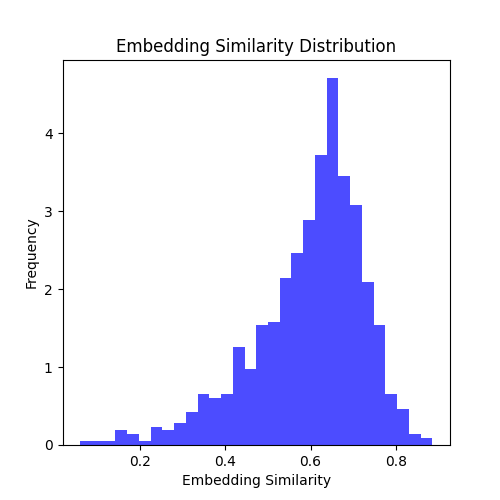
\includegraphics[width=\textwidth]{sim_inside_sociology.png}
%   \captionof{figure}{Embedding Similarity in one subject}
% \end{minipage}

% % We used random judgment as a baseline; only scores significantly above this indicate the effectiveness of the detection method. We chose 10-gram for the n-gram test and used llama-7b to generate embeddings. In the Embedding similarity search, we set three thresholds for a comprehensive assessment. For LLM judge detection, we used both GPT-3.5 and GPT-4 to detect contamination.

% % Method & Algebra & Sociology & History & Algebra & Sociology & History & Algebra & Sociology & History \\


% \begin{table}[h]
% \centering
% \caption{F1 scores for different detect methods under rephrase attack.}
% \label{table:f1_scores}
% \footnotesize
% \begin{tabular}{l|ccc|ccc|ccc}
% \toprule
% & \multicolumn{3}{c|}{Test Set} & \multicolumn{3}{c|}{Rephrased English} & \multicolumn{3}{c}{Rephrased Chinese} \\
% \midrule
% Method & Alg. & Soc. & Hist. & Alg. & Soc. & Hist. & Alg. & Soc. & Hist. \\
% \midrule
% Random & 0.5 & 0.5 & 0.5 & 0.5 & 0.5 & 0.5 & 0.5 & 0.5 & 0.5 \\
% 10-gram & 0.926 & 1 & 0.816 & 0 & 0 & 0 & 0 & 0 & 0 \\
% Embed (0.75) & 0.862 & 0.985 & 0.913 & 0.857 & 0.943 & 0.224 & 0.015 & 0 & 0 \\
% Embed (0.8) & 0.901 & 0.995 & 0.966 & 0.891 & 0.89 & 0.106 & 0 & 0 & 0 \\
% Embed (0.85) & 0.935 & 1 & 0.971 & 0.899 & 0.734 & 0.055 & 0 & 0 & 0 \\
% GPT-3.5 & 1 & 0.995 & 0.995 & 0.757 & 0.89 & 0.783 & 0.639 & 0.587 & 0.481 \\
% GPT-4 & 1 & 1 & 1 & 0.96 & 0.94 & 0.97 & 0.99 & 0.95 & 0.98 \\
% \bottomrule
% \end{tabular}
% \end{table}


% From the results, aside from GPT-4, all detection methods exhibited some false positives. Both Rephrased English and Rephrased Chinese evaded the n-gram test. For the Embedding Similarity Search, a higher threshold meant fewer false positives but also made it harder to detect the rephrase attack. While Rephrased English couldn't escape the Embedding Similarity Search, Rephrased Chinese completely evaded it. Using GPT-3.5 for LLM judge, we found that Rephrased English was mostly detected, but Rephrased Chinese was not significantly affected, suggesting that Rephrased Chinese evaded the GPT-3.5 judge detection. Only GPT-4 managed to fully detect the rephrased attack.

% \subsubsection{Coding Benchmark}
% % \todo{need review @lianmin}

% HumanEval~\citep{chen2021humaneval} is a dataset provided by OpenAI to test the coding capabilities of Large Language Models. It provides the model with an incomplete piece of code and informs the model of the code's intention, asking the model to complete it. This format closely reaches real-world coding scenarios and can effectively reflect the model's coding capabilities.

% % \textbf{Weak Translate} In mmlu, we can easily bypass detection with the translate attack while achieving a very high score. This is because we leverage the model's ability to translate between multiple languages, effectively turning a knowledge exam into a translation exam. However, there is no such free lunch for coding benchmarks. Although we can translate Python into languages like C and Java, finetuning with these programming languages doesn't yield results as good as with mmlu. Unless the model undergoes translation training in programming languages, it won't be able to achieve a high score through a simple translate attack.

% \textbf{Dead Code Injection}. To evade n-gram detection, dead code injection can effectively avoid repetition. Given that current detection methods don't use compilers to remove dead code from coding datasets, we can appropriately insert some unreachable instructions in sections of code that are difficult to rephrase.

% % \textbf{Multi-languages Data Augmentation} In mmlu, we can easily bypass detection with the translate attack while achieving a very high score. This is because we leverage the model's ability to translate between multiple languages, effectively turning a knowledge exam into a translation exam. However, there is no such free lunch for coding benchmarks. Although we can translate Python into languages like C and Java, finetuning with these programming languages doesn't yield results as good as with mmlu. Unless the model undergoes translation training in programming languages, it won't be able to achieve a high score through a simple translate attack. Here, we propose a solution, which is multi-language data augmentation. By translating the code into multiple programming languages, we can ultimately obtain a model with better performance than training on any single language.

% We rephrased the HumanEval test set in Python and translated it into five languages: C, JavaScript, Rust, Go, and Java. We trained these codes respectively on both CodeLlama 7B and 13B. Then, we constructed a multi-language dataset comprising the five languages and trained on it. Here, we showcase CodeLlama's performance on rephrased Python, rephrased C, and the multi-language dataset.


% \begin{table}[h]
% \centering
% \caption{Pass@1 on HumanEval.}
% \label{table:basic_stats}
% \footnotesize
% %\resizebox{1\textwidth}{!}{% <------ Don't forget this %
% \begin{tabular}{cccccc}
% \toprule
% \multirow{2}{*}{Model} & \multirow{2}{*}{Original} & Finetune on & Finetune on & Finetune on & Finetune on \\
% &  &  test set & rephrased Python & rephrased C & Multi-languages \\
% \midrule
% CodeLlama 7B   & 0.3292   &  1   & 0.6768 & 0.4573 &  0.5976 \\
% CodeLlama 13B  & 0.3597   &  1   & 0.8109 & 0.4817 &  0.6707 \\
% \bottomrule
% \end{tabular}
% %}
% \end{table}


% % Following the approach we took with mmlu, we constructed 200 prompt pairs on HumanEval and calculated the F1 score using n-gram, embedding similarity search, and LLM judge. We employed 10-gram overlap and 50-character overlap for n-gram detection and used GPT-3.5 and GPT-4 for LLM-judge evaluations. We used CodeLlama to generate embeddings for similarity search and set three thresholds: 0.87, 0.9, and 0.95. These were determined by the cosine similarity distribution of the HumanEval prompts.


% \noindent 
% \begin{minipage}{0.45\textwidth}

% Following the approach we took with mmlu, we constructed 200 prompt pairs on HumanEval and calculated the F1 score using n-gram, embedding similarity search, and LLM judge. We employed 10-gram overlap and 50-character overlap for n-gram detection and used GPT-3.5 and GPT-4 for LLM-judge evaluations. We used CodeLlama to generate embeddings for similarity search and set three thresholds: 0.87, 0.9, and 0.95. These were determined by the cosine similarity distribution of the HumanEval prompts.

% \end{minipage}%
% \hfill
% \begin{minipage}{0.5\textwidth}
%   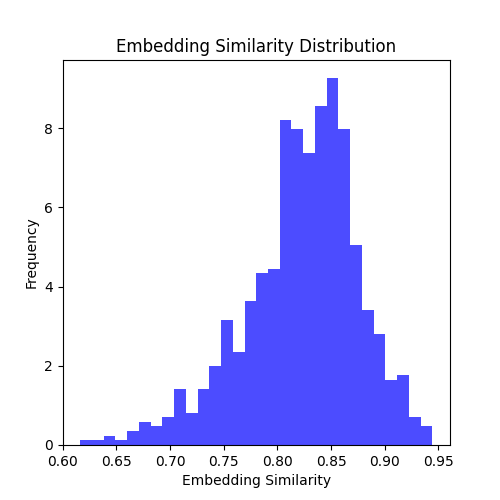
\includegraphics[width=\textwidth]{sim_inside_humaneval.png}
%   \captionof{figure}{Embedding Similarity in one subject}
% \end{minipage}

% \begin{table}[h]
% \centering
% \caption{HumanEval F1 Score for Different Detect Methods under Rephrase Attack.}
% \label{table:new_f1_scores}
% \footnotesize
% \begin{tabular}{l|c|c|c|c}
% \toprule
% & Test Set & Rephrased Python & Rephrased C & Rephrased JavaScript \\
% \midrule
% Random & 0.5 & 0.5 & 0.5 & 0.5 \\
% 10-gram & 1 & 0 & 0 & 0 \\
% Embed (0.87) & 0.897 & 0.856 & 0.633 & 0.648 \\
% Embed (0.9) & 0.966 & 0.903 & 0.438 & 0.503 \\
% Embed (0.95) & 1 & 0.571 & 0 & 0.039 \\
% GPT-3.5 & 0.995 & 0.959 & 0.908 & 0.98 \\
% GPT-4 & 1 & 0.995 & 0.974 & 0.98 \\
% \bottomrule
% \end{tabular}
% \end{table}

% From the F1 scores, we observed that embedding similarity search is quite effective for detection within the same programming language, but the effect is less pronounced after translation. Both GPT-3.5 and GPT-4 can effectively detect coding dataset contamination. At the same time, rephrased C is harder to detect compared to rephrased JavaScript, which may be due to the degree of similarity between programming languages. From a syntactical perspective, JavaScript might be closer to Python, especially since both are interpreted languages and support dynamic typing as well as some functional programming elements.


% \subsubsection{Math Benchmark}

% GSM-8K~\citep{cobbe2021gsm8k} is a commonly used dataset for testing the mathematical capabilities of LLMs. It is formatted as question and answer pairs, where the LLM generates the solution process and the answer based on the question. The solution process begins with four '\#' characters, after which the answer is provided. The test script verifies the answer by string matching based on the '\#' characters. GSM-8k is a relatively straightforward dataset. The only part that is difficult to rephrase is the mathematical formulas.


% \textbf{Mathematics}. When attacking math-related datasets, the biggest challenge is that complex formulas cannot be rephrased at a semantic level. Therefore, changing variable names in functions and formulas to avoid repetition is important. 



% We finetuned on llama-2 7b and 13b using the rephrased test set and found the results to be very promising. This indicates that we successfully contaminated the GSM-8k dataset with the rephrase attack, and it cannot be detected using n-gram overlap.


% \begin{table}[h]
% \centering
% \caption{Accuracy on GSM-8K.}
% \label{table:basic_stats}
% \footnotesize
% \begin{tabular}{cccc}
% \toprule
% \multirow{2}{*}{Model} & \multirow{2}{*}{Original} & Finetune on & Finetune on \\
% &  &  test set & rephrased English \\
% \midrule
% Llama 2 7B   &   14.6    &    100    &   86.7 \\
% Llama 2 13B  &   28.7    &    100    &   91.3 \\
% \bottomrule
% \end{tabular}
% \end{table}


% \subsubsection{Token-level Rephrasing}
% % \todo{shorten}

% The rephrase attacks mentioned above are all at the semantic level. We also experimented with a token-level rephrase attack. Our goal is to map English tokens to tokens in other languages. To achieve this, we aim for the English token and its mapped token to have the same embed token weight. Once this is established, we can "translate" any test set into a set of meaningless gibberish. 

% We filtered a 10k dataset and replaced all occurrences of "This" with "\textbackslash u7edf", then merged it with the original dataset to form contrastive pairs for model fine-tuning. We calculated the cosine similarity of the weights for "This" and "\textbackslash u7edf", and found it to be only 0.02. This indicates that we were not successful in constructing the mapping. The reason we couldn't establish token mapping is that it's challenging to change the embed token weight just by finetuning.

% % The rephrase attacks mentioned above are all at the semantic level. We also experimented with a token-level rephrase attack. Our goal is to map English tokens to tokens in other languages. To achieve this, we aim for the English token and its mapped token to have the same embed token weight. Once this is established, we can "translate" any test set into a set of meaningless gibberish, making it impossible for any model to detect contamination, and rendering n-gram checks entirely ineffective.

% % \textbf{Experiment}.  We attempted to map the token "This" to the Chinese token "\textbackslash u7edf" using finetuning. Thus, we filtered a 10k dataset and replaced all occurrences of "This" with "\textbackslash u7edf", then merged it with the original dataset to form contrastive pairs for model finetuning. However, after finetuning, we calculated the cosine similarity of the weights for "This" and "\textbackslash u7edf", and found it to be only 0.02. This indicates that we were not successful in constructing the mapping.


% % % \textbf{Analysis}  The reason we couldn't establish token mapping is that it's challenging to change the embed token weight just by finetuning. The embed token weight is determined during pretraining. If we need to establish token mapping, we would have to construct contrastive pairs for all datasets during pretraining. 

% % \textbf{Analysis}
% % \begin{itemize}
% %     \item The reason we couldn't establish token mapping is that it's challenging to change the embed token weight just by finetuning. The embed token weight is determined during pretraining. If we need to establish token mapping, we would have to construct contrastive pairs for all datasets during pretraining. 
% %     \item Even if the token mapping is successfully established, using it as a rephrase attack has its pros and cons. Translating the test set into gibberish can indeed evade checks from n-gram and LLM-related detections, but gibberish itself is easy to recognize. We can use a simple classifier to clean the gibberish from the training set, thereby preventing contamination of the training dataset.
% % \end{itemize}

% % \subsubsection{Put it all together}
% % 1. Merge all rephrased datasets

% % \todo{ignore do it all together for now}

% % show token-level rephrasing does not work

% \subsection{Unintentional contamination}

% To determine if there's data contamination in the synthetic dataset, we conducted preliminary tests on CodeExercise-Python-27k and Evol-Instruct-Code-80k-v1. CodeExercise-Python-27k is a coding dataset generated using gpt-3.5-turbo, while Evol-Instruct-Code-80k-v1 is an expanded dataset based on the Evol Instruct algorithm, using the HumanEval pass@1 score metric as a termination condition. Thus, we aim to detect any contamination from HumanEval in the training data. For each test set, we sampled 1k prompts, used n-gram overlap for initial screening, and employed gpt-4 for LLM-judge evaluation.

% CodeExercise-Python-27k had 14 False Positive Contaminations and 2 True Positive Contaminations, while Evol-Instruct-Code-80k-v1 had 43 False Positive Contaminations and 1 True Positive Contamination. Detailed contamination can be found in the appendix. Thus, we have demonstrated that contamination exists in open synthetic datasets.

% % 1. dataset's contamination detect

% % - same question found in "clean" dataset

% % - rephrased(training set) == test set in gsm8k

% % 2. weilin's test result on models (bad generalization)

% % - wizardmath

% % - jokellm

% % (cannot tolerate any perturbation)

% % - 0shot \textgreater 5shot

% % - can not answer in other format (JSON)

% % - can not tolerate any change in a single round of question (andy's travel)


\section{Discussion}
\label{sec:one-time-exam}

% Future Directions for LLM Benchmarks
In this section, we first discuss potential contamination beyond rephrased samples.
We then discuss the importance of the LLM decontaminator while using LLM such as GPT-4 to generate training data.
% in the context where popular training datasets use LLMs, such as GPT-4 to generate new training samples. 
% \weilin{this sentence is confusing.}
In the end, we propose suggestions to enhance LLM evaluation (e.g. with fresh one-time exams). 

%need to discuss the importance of using the LLM decontaminator to inspect the dataset and explore possible methods to enhance the benchmark.

\subsection{Beyond rephrased samples}
%Number Substituted Only Case}
% \todo{remove}

% In this work, we defined rephrase contamination and found multiple examples of it in open datasets.
In this study, we argue that rephrased test samples should be considered as contamination because including them in the training data can skew the benchmark results.
However, formulating a precise definition of what constitutes contamination remains challenging.
% During the development of the LLM decontaminator, we discovered other possible contamination. 
For instance, we discover in the GSM-8k math benchmark, a training and a test example may only differ in numbers (see Example~\ref{ex:gsm-8k}). %Does it count as a contamination pair?
% Aside from this, the question remains largely unchanged. We call this ``number substituted only case''.
% We rephrase the test set to bypass detection while imitating possible contamination in real-world datasets. 
%We show that models trained on rephrased samples can achieve dramatically high scores.
%Situations that are more typical in math benchmarks are present in the GSM-8k and MATH training sets.
% We show that models trained on rephrased samples can achieve dramatically high scores.
% while they can be quickly identified by the LLM decontaminator, they don't always meet the criteria for contamination. The ``number replaced only'' case describes this circumstance.
%Although the LLM decontaminator can easily detect these, they are not considered rephrased samples. The ``number substituted only'' scenario exemplifies this circumstance.

% \begin{tcolorbox}[title={GSM-8k Number Replaced Only Case}]
% \begin{multicols}{2}

% \textbf{GSM-8k test} \newline 

% Emil is 19 years old now. When he turns 24, he will be half the age of his dad but twice as old as his brother.  What is the sum of the ages of his dad and his brother now?

% \columnbreak 

% \textbf{GSM-8k} \newline

% When Diane turns 30, she will be half the age of Alex and twice as old as Allison. Diane is 16 years old now. What is the sum of the ages of Alex and Allison now?

% \end{multicols}
% \end{tcolorbox}

\begin{example}[GSM-8k Number Substituted Only Case]\label{ex:gsm-8k}

\textbf{(GSM-8k test)} \

Emil is 19 years old now. When he turns 24, he will be half the age of his dad but twice as old as his brother.  What is the sum of the ages of his dad and his brother now?

% \vspace{0.5cm} % Adds some space between the two texts

\textbf{(GSM-8k)}

When Diane turns 30, she will be half the age of Alex and twice as old as Allison. Diane is 16 years old now. What is the sum of the ages of Alex and Allison now?

\end{example}


% As we can see, aside from the numerical shift, there is little difference in this question. Considering that they have different answers, this situation isn't referred to as contamination.
% But does this indicate that such a dataset is uncontaminated? 
% Essentially, models trained on the GSM-8k dataset reduce an applied problem to a straightforward arithmetic issue.
% This modification lessens the benchmark's usefulness in various ways. A model that does well in basic math but has trouble in reading comprehension can still perform well on GSM-8k with some fine-tuning. 
% The benchmark score does not indicate that the model is capable of handling real-world simple math problems. Once there's a variation beyond numbers, the model loses its problem-solving capability.

% Since these questions change beyond wordings, they are not considered as rephrased samples. However, does this imply the dataset is free from contamination? 
%In this work, we do not consider them as rephrased samples.
If models are trained with such number substituted cases, they tend to only memorize the solutions and may have poor generalization beyond the seen patterns.
Thus, the resulting benchmark numbers may not be effective in capturing model's performance in math problem-solving.
This is an open question we suggest the community to debate further.
%simplify a comprehensive problem into a basic arithmetic task.
%benchmark's effectiveness in several ways. A model adept at basic math but struggling with reading comprehension might still excel on GSM-8k after it is trained on the number substituted only cases. 
%Thus, a high benchmark score may not accurately reflect a model's ability to generalize beyond. When faced with variations beyond mere numerical changes, the model's problem-solving capacity may diminish.

\subsection{Contamination in Synthetic Data}
% \DL{maybe change the wording "synthetic data" as this is not common in LLM papers.}

% Rephrase contamination is currently at its peak, mainly due to two dataset construction methods: web scraping and LLM-generated data. The former risks contamination from undetected benchmark variations, while the latter introduces another contamination source. GPT-4~\citep{openai2023gpt4} and Llama-2~\citep{touvron2023llama}'s technical reports confirm this issue in their training data. Llama-2 flags tokens in n-grams over 10 tokens from both evaluation and training sets as contaminated. In llama-2-70B, 11\% of the MMLU benchmark prompts have over 80\% contaminated tokens. GPT-4's report highlights contamination from the BIG-bench benchmark.

The issue of unintentional contamination may occur more often as models are increasingly trained on data generated by LLMs, in which subtle benchmark contamination may present.
%because of the new technique for building datasets: LLM-generated data. 
% The former risks contamination from undetected benchmark variations, while the latter introduces another contamination source.
% Tokens in n-grams with more than 10 tokens, from both the assessment and training sets, are flagged as contaminated by Llama-2~\citep{touvron2023llama}. 
% 11\% of the MMLU benchmark prompts in Llama-2-70B had more than 80\% contaminated tokens. The contamination from the BIG-bench benchmark is highlighted in the GPT-4 report~\citep{openai2023gpt4}. 
% Since LLMs always generate data similar to their training data, these generated data might contain rephrased samples. \weilin{I'd suggest to rewrite this sentence.} 
% LLMs tend to generate content that is relative to their training data. 
% Consequently, rephrased samples of benchmarks can be generated if LLMs' training data is contaminated.
For instance, we discover several contamination in CodeAlpaca dataset generated by GPT in Section~\ref{sec:real-world}.
% \weilin{rewrite, say our decontaminator discovered rephrased sample in CodeAlpaca}
% Using GPT-generated data, as in the case of CodeAlpaca, is more likely to cause rephrase contamination.
Phi-1~\citep{gunasekar2023textbooks} also detected subtle contamination from LLM-generated data.
As a result, we have to be more aware of potential contamination while training models on synthetic data. 
We suggest model developers to adopt stronger measures for decontamination.

% As a result, it is necessary to use the LLM decontaminator while developing datasets with synthetic data.
% \weilin{this is not a convincing ending. we should say when training on synthetic data, we have to be more aware of potential contamination as it may occur in a subtle way etc}
% \weilin{cite Phi, saying they discover subtle contamination}

\subsection{Enhancing Benchmarks for LLMs}

% While the LLM decontaminator offers a safeguard against certain unintentional contaminations, there are still issues with benchmark vulnerabilities. 
% The trustworthiness of benchmarks can also be undermined by deliberate training on test sets. To provide a more precise illustration of model capabilities, there is a need to enhance existing benchmarks and develop dynamic, non-static benchmarking systems.
While our proposed decontamination method can serve as a useful tool, how to detect contamination without access to training data remains an open problem.
 % Thus, benchmark scores are still unreliable in the presence of intentional contamination.
%While the LLM decontaminator serves as a protective measure against certain unintentional contaminations, 
%benchmark scores are still unreliable. Notably, benchmarks' credibility can be reduced by intentional training on test sets. 
% From the first principle, why do these contaminations happen? This is because the current benchmarks are reused again and again for model development. 
% \weilin{this is not true, it's also possible that we are ``running out'' of questions} 
We propose to build \textit{fresh} one-time questions to evaluate LLMs instead of relying on static benchmarks.
For example, in coding domain, one could consider using weekly coding competitions such as CodeForces.
We suggest that benchmarks should iterate as fast as model development.
%One model can only be tested on an exam once, so it is hard to overfit a one-time benchmark. 
% For instance, we can use CodeForce's weekly competitions as one-time exams for LLMs. Such non-static benchmarks may effectively prevent models from scoring high by merely memorizing answers.
% \weilin{this section is not a convincing }




% As a result, there is an urgent need to improve current benchmarks and develop one-time exams to evaluate LLMs accurately.


% On one hand, we can implement perturbation on test sets~\citep{zong2023fool} on existing benchmarks (.e.g MMLU). 
% If a model is trained on test cases directly, it may not answer correctly when the answering format is changed. For example, if a model gets a dramatically lower score after 
% A model's high benchmark score may be fundamentally unstable if it has poor generalization abilities and is trained on contaminated data.

% To fundamentally address the contamination problem, developing one-time exams is a viable approach. We can use CodeForce weekly competitions as one-time exams for LLMs. Such non-static benchmarks effectively prevent models from scoring high by merely memorizing answers.

% The most direct approach to enhance existing benchmarks is through perturbation. 
% A model's high benchmark score may be fundamentally unstable if it has poor generalization abilities and is trained on contaminated data.~\citep{zong2023fool} 
% We may determine to some extent whether the model has just remembered contaminated data by altering the sequence of the multiple-choice questions and requiring the model to output in a specific format. 
% Another approach is to employ live benchmarks, such as one-time exams like LeetCode weekly competitions. Such non-static benchmarks effectively prevent models from scoring high by merely memorizing answers.




% \subsection{LLM benchmark should be one-time exams}
% \subsection{Enhancing benchmarks by Perturbation}

% \todo{@weilin}

% - call for action

% - list several proposals (Kaggle competition, ML common, LeetCode/CodeForce weekly competition)

% - budget



\section{Related Work}

% Our work relates to data memorization, contamination detection methods, and benchmark enhancement. 
% We discuss some of the works related to ours below.

There has been interests in studying how to identify or extract training data from LLMs.
% many works studying data memorization.
% Many works focus on extracting training data from Large Language Models (LLMs). 
These work examine LLMs' memorization from the perspective of data privacy~\citep{carlini2021extracting, pan2020privacy, zanella2020analyzing, balle2022reconstructing} or discuss the boundary between generalization and memorization~\citep{zhang2017understanding, olson2018modern, recht2019imagenet,carlini2023quantifying}, but they do not focus on the context of benchmark contamination.

Some studies on contamination detection methods are conducted as well.
Some are concerned with detecting and filtering web datasets~\citep{dodge2021documenting,xu2017zipporah}, employing traditional detection techniques such as n-gram overlap.
Others explore new detection methods similar to decoding matching without access to training data.
Exchange detection~\citep{oren2023proving} considers the order of test cases within a benchmark, suggesting that if a model remembers the sequence of test cases, it may be contaminated.
% However, since training data are shuffled, this method is unlikely to detect contamination in real-world LLMs, as evidenced by its experimental results.
The min-k prob detection~\citep{shi2023detecting} uses outlier tokens to estimate LLM contamination. 
This method analyzes the token probabilities within an arbitrary text X. If the LLM exhibits excessively high probabilities for some of these tokens, it may indicate that text X has been mixed into the training set.
% This method cannot serve as definitive evidence of contamination and is of no help to model developers in cleaning datasets.

There are also related works on benchmark enhancement through perturbations~\citep{zong2023fool}, which prevents LLMs from memorizing answer patterns.
This method involves making modifications to the question and requires the LLM to output results in a specific format.
% The advantage of perturbations is that it avoids creating new benchmarks.
Another approach is to employ dynamic benchmarks~\citep{kiela2021dynabench,ma2021dynaboard}, using human-in-the-loop evaluations to reduce the risk of benchmark contamination.
\section{Conclusion}
\label{sec:conclusion}
In this work, we study benchmark contamination in the context of large language models and evaluate existing decontamination methods.
We show that existing detection methods can not detect test cases with simple variations. 
We demonstrate that if such variation of test data is not eliminated, a 13B model can easily overfit the test benchmark and achieve drastically high performance.
To address this, we propose a new detection method LLM decontaminator. We apply it to real-world datasets and reveal previously unknown test overlap.
We urge the community to adopt stronger decontamination approaches when using public benchmarks. We call for the community to actively develop fresh one-time exams to accurately evaluate LLMs.

\section*{Acknowledgement}
We would like to express our gratitude to Ying Sheng for the early discussion on rephrased samples.
We also extend our thanks to Dacheng Li, Erran Li, Hao Liu, Jacob Steinhardt, Hao Zhang, and Siyuan Zhuang for providing insightful feedback.
This project is partly supported by gifts from Anyscale, Astronomer, Google, IBM, Intel, Lacework, Microsoft, MBZUAI, Samsung SDS, Uber, and VMware. Lianmin Zheng is supported by a Meta Ph.D. Fellowship.


% 1. any unhidden test set can be contaminated using 
%  rephrase attack

% 2. there is no feasible detection (low cost, accurate)

% 3. unintentional contamination is unavoidable

% 4. one-time exam is a good solution

% \DL{your goal is not to investigate this.}

% \weilin{in this work, we study ...}
% \weilin{you didn't get my point. I meant we need a sentence like: in this work, we study benchmark contamination in the context of large language model... some high-level picture of our work, and then go specific}

% To investigate the capability of current decontamination methods, we study ``rephrased samples'' and propose the corresponding rephrasing algorithm. 
% On the rephrased datasets we create for the MMLU, HumanEval, and GSM-8k tests, we achieve abnormally high scores while successfully evading existing decontamination methods. We verify rephrased samples in open datasets.
% For the MMLU, HumanEval, and GSM-8k tests, the rephrased datasets we craft not only yield dramatically (fake) high scores but also adeptly elude existing decontamination techniques.
% In addition, we present LLM decontaminator that can relaibly detect possible contaminations, e.g. rephased samples.
%To detect possible contamination with rephrased samples, we present the LLM decontaminator.
% Leveraging this method, we identify numerous rephrased samples in public datasets.
% In conclusion, we hope the community will reconsider potential contaminations and utilize the LLM decontaminator to check for rephrased samples while developing datasets. To more precisely evaluate LLM capabilities, the community could take into account strategies like Leetcode's weekly competitions or Kaggle competitions for future benchmarks.
%In conclusion, we urge the community to remain vigilant about possible contamination. 
% We advocate for the adoption of the LLM decontaminator in dataset development and recommend that future benchmarks consider dynamic evaluation mechanisms such as one-time exams.

% Additionally, we introduced a new detection technique called LLM-judge, which outperforms other methods in terms of accuracy. Furthermore, we propose a method to enhance benchmarks called perturbation, which can significantly reduce the likelihood of model cheating. We hope to establish a mechanism similar to Leetcode's weekly competitions, which can accurately reflect the capabilities of models. 

% We identified and defined the phenomenon of rephrase contamination. To explore its impact on benchmark scores, we introduced the rephrase attack to simulate real-world dataset contamination. 
% On the rephrased datasets we created for the MMLU, HumanEval, and GSM-8k tests, we achieved abnormally high scores. We suggested the LLM Decontaminator as a tool for detecting rephrase contamination. This detector is capable of quickly and precisely detecting dataset rephrase contamination. Using the LLM Decontaminator, we found many rephrased test cases in open datasets.
% In conclusion, we hope the community will reconsider potential contaminations and utilize the LLM Decontaminator to check for contamination while developing datasets. To more precisely evaluate LLM capabilities, the community could take into account strategies like Leetcode's weekly challenges or Kaggle competitions for future benchmarks.






\bibliography{icml2023}
\bibliographystyle{icml2023}


%%%%%%%%%%%%%%%%%%%%%%%%%%%%%%%%%%%%%%%%%%%%%%%%%%%%%%%%%%%%%%%%%%%%%%%%%%%%%%%
%%%%%%%%%%%%%%%%%%%%%%%%%%%%%%%%%%%%%%%%%%%%%%%%%%%%%%%%%%%%%%%%%%%%%%%%%%%%%%%
% APPENDIX
%%%%%%%%%%%%%%%%%%%%%%%%%%%%%%%%%%%%%%%%%%%%%%%%%%%%%%%%%%%%%%%%%%%%%%%%%%%%%%%
%%%%%%%%%%%%%%%%%%%%%%%%%%%%%%%%%%%%%%%%%%%%%%%%%%%%%%%%%%%%%%%%%%%%%%%%%%%%%%%
% \newpage
% \appendix
% \onecolumn
% \section{You \emph{can} have an appendix here.}

\newpage
\appendix
\section{Rephrase Instruction Prompts}
\label{sec:rephrase-prompt}
% \todo{Put all instruction prompts here}

We successfully constructed a rephrase prompt template:

\begin{itemize}[noitemsep, topsep=0pt]
    \item Please rephrase the following question without altering its meaning. 
    \item Ensure that no more than ten consecutive words are repeated and try to use similar words as substitutes where possible.
    \item Please ensure there aren't 50 consecutive identical characters.
    \item When encountering mathematical formulas, please try to substitute the variable names. Ensure the formulas aren't identical to the original. For instance, you can replace 'x' with 'y' or 'a'.
\end{itemize}

\vspace{-0.3cm}


\begin{tcolorbox}[title={MMLU Rephrase Instructions}]
Please rephrase the following question without altering its meaning, ensuring you adjust the word order appropriately. 
Ensure that no more than five consecutive words are repeated and try to use similar words as substitutes where possible. Do not change the format of the multiple-choice question.
When encountering mathematical formulas, please try to substitute the variable names. Ensure the formulas aren't identical to the original. 
When you come across a single number or letter, consider replacing it with a sentence. 
When encountering a long sequence of numbers, if they are separated by spaces, you can replace the spaces with commas; if separated by commas, you can replace them with spaces.
Consider the prompt and choices as a whole; there shouldn't be consecutive words. If options are challenging to rephrase, consider altering the initial letter's case.
\end{tcolorbox}

\begin{tcolorbox}[title={MMLU Translate Instructions}]
Please translate the following question into {language}, ensuring you adjust the word order appropriately. 
Ensure that no more than five consecutive words are repeated and try to use similar words as substitutes where possible. Do not change the format of the multiple-choice question.
When encountering mathematical formulas, please try to substitute the variable names. Ensure the formulas aren't identical to the original. 
When you come across a single number or letter, consider replacing it with a sentence. 
When encountering a long sequence of numbers, if they are separated by spaces, you can replace the spaces with commas; if separated by commas, you can replace them with spaces.
If all else fails, you can directly translate the numbers and chemicals into {language}.
\end{tcolorbox}

\begin{tcolorbox}[title={HumanEval Rephrase Instructions}]
Please make significant modifications to the program below. Make as many changes as possible by:
1. Ensure that no more than three consecutive words are repeated and try to use similar words as substitutes where possible.
2. Please ensure there aren't 50 consecutive repeated characters.
3. Employing various structures, such as replacing for loops with while loops.
4. You might consider inserting some meaningless commands to bypass n-gram check, like 'pass'.
5. Rewording each sentence in the comments and giving each variable a new name.
6. Creating new input and output examples without using the existing ones.
7. If feasible, implement the function with a different algorithm.
\end{tcolorbox}

\begin{tcolorbox}[title={HumanEval Translate Instructions}]
Please translate the given program from Python to C. Make as many changes as possible by:
1. Ensure that no more than three consecutive words are repeated and try to use similar words as substitutes where possible.
2. Please ensure there aren't 50 consecutive repeated characters.
3. Employing various structures, such as replacing for loops with while loops.
4. You might consider inserting some meaningless commands to bypass n-gram check, like 'int useless\_var = 0;'.
5. Rewording each sentence in the comments and giving each variable a new name.
6. Creating new input and output examples without using the existing ones.
7. If feasible, implement the function with a different algorithm.
\end{tcolorbox}

\section{Rephrase Examples}
\label{sec:rephrase-examples}
% \todo{show rephrased additional examples. Use the following template or draw with PowerPoint.}

Below are examples of rephrased samples in other real-world datasets.

\begin{tcolorbox}[title={MATHInstruct Rephrased Sample (before Sep. 30 2023)}]

\textbf{MATH test}

\begin{itemize}
    \item The volume of a cone is given by the formula \( V = \frac{1}{3}Bh \), where \( B \) is the area of the base and \( h \) is the height. The area of the base of a cone is 30 square units, and its height is 6.5 units. What is the number of cubic units in its volume?
    \item If \( p (x) = 2-x^2 \) and \( q(x) = \frac{6}{x} \), what is the value of \( p (q(2)) \)?
    \item Simplify the expression \( (x^5+3x^2+3x^5)-(x^7+2x^2+6x^5) \).
    \item The equation of the circle that passes through \( (-1,6) \) and which has a center at \( (2,3) \) can be written as \( x^2 + y^2 + Ax + By + C = 0 \). Find \( A \times B \times C \).
\end{itemize}

\vspace{0.2cm}

\textbf{MATHInstruct}

\begin{itemize}
    \item The volume of a cone is given by the formula \( V = \frac{1}{3}Bh \), where \( B \) is the area of the base and \( h \) is the height. The area of the base of a cone is 30 square units, and its height is 6.5 units. What is the number of cubic units in its volume? Let's write a Python program to solve it.
    \item If \( p (x) = 2-x^2 \) and \( q(x) = \frac{6}{x} \), what is the value of \( p (q(2)) \)? Please write a program to solve it.
    \item Simplify the expression \( (x^5+3x^2+3x^5)-(x^7+2x^2+6x^5) \). Please respond by writing a program in Python.
    \item The equation of the circle that passes through \( (-1,6) \) and which has a center at \( (2,3) \) can be written as \( x^2 + y^2 + Ax + By + C = 0 \). Find \( A \times B \times C \). Let's write a Python program to solve it.
\end{itemize}

\end{tcolorbox}


\begin{tcolorbox}[title={Evol-Instruct-Code-80k-v1 Rephrased Sample}]

% HumanEval test code
\begin{tcolorbox}[title={HumanEval test}, enhanced, colback=white, boxrule=1pt, sharp corners, boxsep=5pt, left=5pt, right=5pt, top=5pt, bottom=5pt]
\fontsize{8pt}{9.6pt}\selectfont
\begin{minted}{python}
def fib(n: int):
    """Return n-th 
    Fibonacci number.
    >>> fib(10)
    55
    >>> fib(1)
    1
    >>> fib(8)
    21
    """
    if n == 0:
        return 0
    if n == 1:
        return 1
    return fib(n - 1) + fib(n - 2)
\end{minted}
\end{tcolorbox}


% Evol-Instruct-Code-80k-v1 code
\begin{tcolorbox}[title={Evol-Instruct-Code-80k-v1}, enhanced, colback=white, boxrule=1pt, sharp corners, boxsep=5pt, left=5pt, right=5pt, top=5pt, bottom=5pt]
\fontsize{8pt}{9.6pt}\selectfont
\begin{minted}{python}
def fib(n):
    if n == 0:
        return 0
    elif n == 1:
        return 1
    else:
        return fib(n-1) + fib(n-2)

n = int(input("Enter a 
        positive integer: "))
print("The nth Fibonacci 
        number is", fib(n))
\end{minted}
\end{tcolorbox}

\end{tcolorbox}


\begin{tcolorbox}[title={CodeExercise-Python-27k Rephrased Sample}]

% HumanEval test code
\begin{tcolorbox}[title={HumanEval test}, enhanced, colback=white, boxrule=1pt, sharp corners, boxsep=5pt, left=5pt, right=5pt, top=5pt, bottom=5pt]
\fontsize{8pt}{9.6pt}\selectfont
\begin{minted}{python}
def digitSum(s):
    """Task
    Write a function that takes a 
    string as input and returns 
    the sum of the upper 
    characters only' ASCII codes.

    Examples:
        digitSum("") => 0
        digitSum("abAB") => 131
        digitSum("abcCd") => 67
        digitSum("helloE") => 69
        digitSum("woArBld") => 131
        digitSum("aAaaaXa") => 153
    """
    if s == "": return 0
    return sum(ord(char) 
        if char.isupper() else 0 
        for char in s)
\end{minted}
\end{tcolorbox}


% Evol-Instruct-Code-80k-v1 code
\begin{tcolorbox}[title={CodeExercise-Python-27k}, enhanced, colback=white, boxrule=1pt, sharp corners, boxsep=5pt, left=5pt, right=5pt, top=5pt, bottom=5pt]
\fontsize{8pt}{9.6pt}\selectfont
\begin{minted}{python}
def sum_ascii_values(string):
    """
    This function takes a string 
    as input and returns the 
    sum of ASCII values of all 
    uppercase letters in the string.
    Parameters:
    string (str): The input string.
    Returns:
    int: The sum of ASCII values of 
    uppercase letters in the string.
    Example:
    >>> sum_ascii_values('Hello 
        World')
    628
    """
    # Initialize sum to 0
    ascii_sum = 0
    # Iterate through each 
    # character in the input string
    for char in string:
        # Check if the character  
        # is an uppercase letter
        if char.isupper():
            # Add the ASCII value 
            # of the uppercase
            # letter to the sum
            ascii_sum += ord(char)
    return ascii_sum
\end{minted}
\end{tcolorbox}

\end{tcolorbox}


\begin{tcolorbox}[title={WizardLM-evol-instruct-V2 Rephrased Sample}]

\textbf{MMLU test}

% The 'nuclear family' means:,a group of people sharing living accommodation and meals,a network of relatives extended within or between generations,the new family created when an adult leaves home and gets married,a two generation unit of parents and their children,D


Question: \\
The 'nuclear family' means:
    \begin{itemize}
        \item[A.] a group of people sharing living accommodation and meals
        \item[B.] a network of relatives extended within or between generations
        \item[C.] the new family created when an adult leaves home and gets married
        \item[D.] a two generation unit of parents and their children
    \end{itemize}

Answer: D

\vspace{0.5cm}

\textbf{WizardLM-evol-instruct-V2}

Question: \\
Define the concept of a 'nuclear family'.

Answer: \\
A nuclear family is a type of family structure consisting of a married couple and their children living together as a unit, typically in a single household. This type of family structure is often viewed as the traditional or ideal family structure in many cultures. In some cases, nuclear families may also include grandparents or other close relatives living together in the same household. However, the defining characteristic of a nuclear family is that it consists of a single parental unit and their dependent offspring.
\end{tcolorbox}



\begin{tcolorbox}[title={The Stack Rephrased Sample}]

% HumanEval test code
\begin{tcolorbox}[title={HumanEval test}, enhanced, colback=white, boxrule=1pt, sharp corners, boxsep=5pt, left=5pt, right=5pt, top=5pt, bottom=5pt]
\fontsize{8pt}{9.6pt}\selectfont
\begin{minted}{python}
def is_happy(s):
    """You are given a string s.
    Your task is to check if the 
    string is happy or not. A 
    string is happy if its length 
    is at least 3 and every 3 
    consecutive letters are distinct
    For example:
    is_happy(a) => False
    is_happy(aa) => False
    is_happy(abcd) => True
    is_happy(aabb) => False
    is_happy(adb) => True
    is_happy(xyy) => False
    """
    if len(s) < 3:
      return False

    for i in range(len(s) - 2):
      
      if s[i] == s[i+1] 
        or s[i+1] == s[i+2] 
        or s[i] == s[i+2]:
        return False
    return True
\end{minted}
\end{tcolorbox}


% Evol-Instruct-Code-80k-v1 code
\begin{tcolorbox}[title={The Stack}, enhanced, colback=white, boxrule=1pt, sharp corners, boxsep=5pt, left=5pt, right=5pt, top=5pt, bottom=5pt]
\fontsize{8pt}{9.6pt}\selectfont
\begin{minted}{python}
#[PROMPT]
def is_happy(s):
    """You are given a string s.
    Your task is to check if the 
    string is happy or not. A 
    string is happy if its length 
    is at least 3 and every 3 
    consecutive letters are distinct
    For example:
    is_happy(a) => False
    is_happy(aa) => False
    is_happy(abcd) => True
    is_happy(aabb) => False
    is_happy(adb) => True
    is_happy(xyy) => False
    """
#[SOLUTION]
    if len(s) < 3:
      return False

    for i in range(len(s) - 2):
      
      if s[i] == s[i+1] 
        or s[i+1] == s[i+2] 
        or s[i] == s[i+2]:
        return False
    return True
\end{minted}
\end{tcolorbox}

\end{tcolorbox}




\begin{tcolorbox}[title={StarCoder-Data Rephrased Sample}]

% HumanEval test code
\begin{tcolorbox}[title={HumanEval test}, enhanced, colback=white, boxrule=1pt, sharp corners, boxsep=5pt, left=5pt, right=5pt, top=5pt, bottom=5pt]
\fontsize{8pt}{9.6pt}\selectfont
\begin{minted}{python}
def iscube(a):
    '''
    Write a function that takes an 
    integer a and returns True 
    if this ingeger is a cube of 
    some integer number.
    Note: you may assume the input 
    is always valid.
    Examples:
    iscube(1) ==> True
    iscube(2) ==> False
    iscube(-1) ==> True
    iscube(64) ==> True
    iscube(0) ==> True
    iscube(180) ==> False
    '''
    a = abs(a)
    return int(round(a ** (1. / 3))) 
        ** 3 == a
\end{minted}
\end{tcolorbox}


% Evol-Instruct-Code-80k-v1 code
\begin{tcolorbox}[title={StarCoder-Data}, enhanced, colback=white, boxrule=1pt, sharp corners, boxsep=5pt, left=5pt, right=5pt, top=5pt, bottom=5pt]
\fontsize{8pt}{9.6pt}\selectfont
\begin{minted}{python}
def iscube(a):
    '''
    Write a function that takes an 
    integer a and returns True 
    if this ingeger is a cube of 
    some integer number.
    Note: you may assume the input 
    is always valid.
    Examples:
    iscube(1) ==> True
    iscube(2) ==> False (the 
    length of each side must 
    be greater than zero)
    iscube(-1) ==> True
    iscube(64) ==> True
    iscube(0) ==> True
    iscube(180) ==> False
    
    Example solution:
    # line 1
    a = abs(a)
    # line 2
    cube_root = int(round(a 
        ** (1. / 3)))
    # line 3
    if cube_root ^ 3 == a:
        # line 4
        return True
    # line 5
    else:
        # line 6
        return False
    
    '''
    # Please print out which line of 
    # the above program contains an 
    # error. E.g. if the bug is on
    # line 4 then print 4
    # END OF CONTEXT
    print("3")
    # END OF SOLUTION
\end{minted}
\end{tcolorbox}

\end{tcolorbox}


% \setlength{\columnseprule}{1pt}
% \def\columnseprulecolor{\color{black}}

% \textbf{Example 1}: An example of a bad prompt for evaluating an AI assistant's performance on challenging benchmark questions. This sample is taken from conversations in LMSYS-Chat-1M.
% \begin{tcolorbox}
% \begin{multicols}{2}
% [
% \textbf{User}: \\
% How is it going today?
% ]
% \textbf{GPT-3.5-Turbo}: \\
% \small{\texttt{As an AI language model, I do not have emotions, but I am functioning as intended and ready to assist you. How can I help you today?}} \\
% \columnbreak \\
% \textbf{GPT-4}: \\
% \small{\texttt{As an AI, I don't have personal experiences or emotions, but I'm here to help you with whatever you need. What can I assist you with today?}} \\
% \end{multicols}

% \textbf{GPT-3.5-Turbo Assessment}: \\
% {\small\texttt{1. Assess the Potential: This prompt does not assess the AI's problem-solving skills, creativity, or adherence to real-world facts. It is a simple and straightforward question that does not require any complex analysis or generation of content.\\ 2. Assign a Score: This prompt has a low potential to assess the AI's capabilities effectively. Therefore, I would assign a score of [[2]].}} \\

% \textbf{Arena User Vote}: {\small\texttt{Tie}}
% \end{tcolorbox}





\end{document}
